%%
%% Copyright 2019-2021 Elsevier Ltd
%%
%% This file is part of the 'CAS Bundle'.
%% --------------------------------------
%%
%% It may be distributed under the conditions of the LaTeX Project Public
%% License, either version 1.2 of this license or (at your option) any
%% later version.  The latest version of this license is in
%%    http://www.latex-project.org/lppl.txt
%% and version 1.2 or later is part of all distributions of LaTeX
%% version 1999/12/01 or later.
%%
%% The list of all files belonging to the 'CAS Bundle' is
%% given in the file `manifest.txt'.
%%
%% Template article for cas-sc documentclass for
%% single column output.

\documentclass[a4paper,fleqn]{cas-sc}

% If the frontmatter runs over more than one page
% use the longmktitle option.

%\documentclass[a4paper,fleqn,longmktitle]{cas-sc}

\usepackage[numbers]{natbib}
%\usepackage[authoryear]{natbib}
%\usepackage[authoryear,longnamesfirst]{natbib}
%%%Author macros
\def\tsc#1{\csdef{#1}{\textsc{\lowercase{#1}}\xspace}}
\tsc{WGM}
\tsc{QE}
%%%

% Uncomment and use as if needed
%\newtheorem{theorem}{Theorem}
%\newtheorem{lemma}[theorem]{Lemma}
%\newdefinition{rmk}{Remark}
%\newproof{pf}{Proof}
%\newproof{pot}{Proof of Theorem \ref{thm}}

\begin{document}
\let\WriteBookmarks\relax
\def\floatpagepagefraction{1}
\def\textpagefraction{.001}

% Short title
\shorttitle{Impact of Iron Defect Variability on Silicon Solar Cell Performance}

% Short author
\shortauthors{O.Olikh, O.Zavhorodnii}

% Main title of the paper
\title [mode = title]{Modeling the Impact of Iron Defect Variability on Silicon Solar Cell Performance Across Different Scenarios}

% Title footnote mark
% eg: \tnotemark[1]
%\tnotemark[<tnote number>]

% Title footnote 1.
% eg: \tnotetext[1]{Title footnote text}
%\tnotetext[<tnote number>]{<tnote text>}

% First author
%
% Options: Use if required
% eg: \author[1,3]{Author Name}[type=editor,
%       style=chinese,
%       auid=000,
%       bioid=1,
%       prefix=Sir,
%       orcid=0000-0000-0000-0000,
%       facebook=<facebook id>,
%       twitter=<twitter id>,
%       linkedin=<linkedin id>,
%       gplus=<gplus id>]

%\author[1,3]{Oleg Olikh}[type=Co-ordinator,
%       style=chinese,
%       auid=000,
%       bioid=1,
%       prefix=Dr.,
%       orcid=0000-0003-0633-5429,
%%       facebook=<facebook id>,
%%       twitter=<twitter id>,
%%       linkedin=<linkedin id>,
%       gplus=<gplus id>]
\author{Oleg Olikh}[
%       type=Co-ordinator,
%       style=chinese,
%       auid=000,
%       bioid=1,
%       prefix=Dr.,
       orcid=0000-0003-0633-5429
       % ,
%       facebook=<facebook id>,
%       twitter=<twitter id>,
%       linkedin=<linkedin id>,
%       gplus=<gplus id>
       ]

% Corresponding author indication
\cormark[1]

% Footnote of the first author
%\fnmark[1]

% Email id of the first author
\ead{olegolikh@knu.ua}

% URL of the first author
%\ead[url]{https://gen.phys.knu.ua/280-olikh/}

% Credit authorship
% eg: \credit{Conceptualization of this study, Methodology, Software}
%\credit{<Credit authorship details>}

% Address/affiliation
\affiliation{organization={Taras Shevchenko National University of Kyiv},
            addressline={64/13, Volodymyrska Street},
            city={Kyiv},
%          citysep={}, % Uncomment if no comma needed between city and postcode
            postcode={01601},
 %           state={},
            country={Ukraine}}

%\affiliation[<aff no>]{organization={Taras Shevchenko National University of Kyiv, Faculty of Physics},
%            addressline={ave Glushkov 2},
%            city={Kyiv},
%%          citysep={}, % Uncomment if no comma needed between city and postcode
%            postcode={03022},
%            state={},
%            country={Ukraine}}

%\author[1,3]{Zavhorodnii Oleksii}[type=editor,
%       style=chinese,
%       auid=000,
%       bioid=1,
%%       prefix=Mr,
%       orcid=0000-0001-8080-7661,
%%       facebook=<facebook id>,
%%       twitter=<twitter id>,
%%       linkedin=<linkedin id>,
%       gplus=<gplus id>]

\author{Oleksii Zavhorodnii}[
       orcid=0000-0001-8080-7661]

% Footnote of the second author
%\fnmark[2]

% Email id of the second author
\ead{nevermor464@gmail.com}

% URL of the second author
%\ead[url]{https://gen.phys.univ.kiev.ua/}

% Credit authorship
%\credit{}

% Address/affiliation
%\affiliation[<aff no>]{organization={Taras Shevchenko National University of Kyiv, Faculty of Physics},
%            addressline={ave Glushkov 2},
%            city={Kyiv},
%%          citysep={}, % Uncomment if no comma needed between city and postcode
%            postcode={03022},
%            state={},
%            country={Ukraine}}

% Corresponding author text
%\cortext[1]{Corresponding author}

% Footnote text
%\fntext[1]{}

% For a title note without a number/mark
%\nonumnote{}

% Here goes the abstract
\begin{abstract}
Transitioning to renewable energy sources is paramount for humanity's sustainable development, and silicon solar cells are at the forefront of solar energy conversion.
Iron in these structures is a primary one of the most detrimental metallic impurities.
This study examines the impact of iron defect variability on silicon solar cell performance across various scenarios.
%integrating simulation and experimental validation.
We have simulated solar cells using SCAPS software across a range of temperatures $(290-340)$~K,
base thicknesses $(180-380)$~$\mu$m, doping levels ($10^{15} - 10^{17}$)~cm$^{-3}$,
with iron concentrations varying from $10^{10}$ to $10^{14}$~cm$^{-3}$ under AM1.5 and monochromatic (940~nm) illumination.
Analyzed across all cases were the effects of iron-boron pair dissociation on short-circuit current, open-circuit voltage, fill factor, and efficiency.
The experimental measurements validated the simulation results, demonstrating good agreement for all photovoltaic parameters.
This study investigates the potential of using photovoltaic parameter changes induced by iron-related defect restructuring to estimate iron concentration.
It is shown that changes in short-circuit current obtained under monochromatic illumination are the most reliable,
while the fill factor is the least effective.
Principal component analysis was used to estimate the number of independent variables when multiple photovoltaic parameters are used simultaneously.
\end{abstract}



% Use if graphical abstract is present
%\begin{graphicalabstract}
%\includegraphics{}
%\end{graphicalabstract}

% Research highlights
\begin{highlights}
\item The iron defect transformation effect on Si solar cells' performance was studied using SCAPS simulation
\item Short-circuit current changes are most suitable for estimating iron impurity concentration.
\item Open-circuit voltage changes are a non-monotonic function of iron concentration at low doping levels.
\item Monochromatic illumination is more effective than AM1.5 for accurate iron concentration estimation.
\end{highlights}


% Keywords
% Each keyword is seperated by \sep
\begin{keywords}
 silicon\sep iron-boron pairs\sep solar cells \sep SCAPS \sep simulation \sep defect influence \sep estimation of iron contamination
\end{keywords}

\maketitle

% Main text
\section{Introduction}%\label{}
\par
The necessity for renewable energy sources to meet the growing global demand for sustainable and environmentally friendly energy alternatives has become evident.
Among the wide range of renewable energy sources, sunlight is the cleanest, safest,
and most abundant source for use in sustainable energy to support economic growth \cite{PratapSingh2019}.
The utilization of solar energy heavily depends on the use of photovoltaic cells, with silicon--based devices playing a critical role \cite{Basnet2024,Wang2024}.


The issue of semiconductor purity has become increasingly significant since the advent of the transistor in 1947 \cite{Claers2018}.
The 1960 study by Shockley and Queisser \cite{Goetzberger1960} demonstrated that
the electrical properties of $n^{+}-p$ silicon diodes deteriorate when impurity atoms of metals such as Cu, Fe, Mn, Au, Zn, and Ni are present.
This study prompted investigations focused on preventing contaminating metals from entering semiconductors during manufacturing.
In particular, metallic impurities are known to reduce the efficiency of
silicon--based devices through direct shunting \cite{Rsh:Breitenstein},
increased leakage current \cite{Lee1980},
or bulk recombination \cite{Istratov2000}.
Despite extensive study of metallic impurities in silicon over the past fifty years \cite{Claers2018,Pearce1977},
the problem continues to attract significant attention \cite{Hajjiah2020,Le2024,Maoudj2021,OlikhPSSA,LaineIEEEPV2016}.


Iron is prominent among metallic contaminants, with its atoms being among
the most prevalent and detrimental impurities in silicon solar cells (SSCs) \cite{Buonassisi2006}.
Even in small concentrations (about $10^{10}$~cm$^{-3}$),
point defects related to Fe can significantly influence the performance of SSCs \cite{IronSC,Herguth2022}.
Therefore, it is of critical importance to assess the concentration of iron impurities.
In response to this challenge, various methodologies have been put forward,
often based on the property of iron atoms to form pairs with acceptors.
In particular, iron atoms are predominantly located in interstitial positions in silicon, forming the Fe$_i$ defect.
In $p$--type crystals, without external illumination, iron atoms carry positive charges and tend to bond with negatively charged doping atoms
(boron, aluminum, gallium, or indium), forming Fe$_i$B$_\mathrm{Si}$ pairs \cite{Kimerling1983}.
However, these pairs can destabilized by intense illumination, electron injection, or heating up to 200~$^\circ$C \cite{FeBAssJAP2014}.
The recombination properties of iron-related defects Fe$_i$ and Fe$_i$B$_s$ differ significantly,
which profoundly affects the overall characteristics of the crystal.
This fact formed the basis for the first method of assessing iron concentration \cite{Zoth1990},
which relied on measuring the diffusion length of minority carriers using the surface photovoltage method \cite{Tousek2008}.
Many other methods involve measurements of carrier lifetime \cite{Rein2,Schmidt2005},
Quasi-Steady-State Photoconductance \cite{Goodarzi2017},
or the study of kinetic dependencies of short-circuit current \cite{Olikh2021JAP}
or photoluminescence intensity \cite{FeMethod2012} during the reaction Fe$_i$B$_\mathrm{Si}$ $\rightleftarrows$ Fe$_i$ + B$_\mathrm{Si}$.


Notably, the presence of Fe--related defects affects the dynamics of electron and hole movement within the solar cell,
which is reflected in changes to the appearance of the current--voltage ($I$-$V$) characteristics of SSCs overall,
as well as modifications to the main photoelectric parameters
(short-circuit current  $I_\mathrm{SC}$,
open-circuit voltage $V_\mathrm{OC}$,
efficiency $\eta$, and fill factor $F\!F$)
in particular.
These findings create fundamental possibilities to advance methods for estimating iron concentration by $I$-$V$ curves measuring before and after pair dissolution.
The advantages of such an approach are associated with the possibility of directly characterizing finished solar cells,
as well as the absence of the need for additional equipment other than that required for $I$-$V$ measurements, which is extremely common.
Efforts have been made initially in developing such methods.
For instance, it was proposed to estimate the concentration of iron in SSCs based on changes in the ideality factor \cite{Olikh2019SM,Olikh2022PPV}
or open-circuit voltage \cite{Herguth2022}.
However, developing such approaches requires evaluating how a particular parameter changes when iron--containing pairs dissolve
and determining whether it can estimate the iron concentration $N_\mathrm{Fe}$.
For example, the most evident conditions for utilizing a specific parameter include its change due to the transformation
Fe$_i$B$_\mathrm{Si}$ $\rightarrow$ Fe$_i$ +B$_\mathrm{Si}$,
at least by 10~\%, along with a monotonic dependence of these changes on $N_\mathrm{Fe}$.


This paper intends to determine the variations of $I_\mathrm{SC}$, $V_\mathrm{OC}$, $\eta$, and $F\!F$
resulting from the decay of iron-containing pairs in boron-doped silicon solar cells.
Previous similar calculations have been conducted \cite{FeB:Schmidt,IronSC,Hajjiah2020},
but the results presented typically pertain only to certain temperatures,
illumination levels (often AM1.5), and solar cells with specific parameters.
In this study, we performed calculations over a sufficiently wide temperature range (290-340~K)
and for solar cells with varying base thickness (180-380~$\mu$m) and doping levels
(boron concentration in the base ranging from $10^{15}$ to $10^{17}$~cm$^{-3}$).
The results obtained allow us to assess the feasibility and potential of using the
main photovoltaic parameters of specific solar cells to estimate the $N_\mathrm{Fe}$ value across a range of temperatures,
including conditions similar to those encountered in typical SSC applications.
Furthermore, investigations have explored changes in photoelectric performance under not only solar illumination (AM1.5G)
but also low-intensity monochromatic light (wavelength of 940~nm, intensities of 5~W/m$^{2}$ and 10~W/m$^{2}$).
In the first case, while it is customary to adhere to standard conditions,
it's essential to consider that illumination at 1000~W/m$^{2}$ can lead to the decay of Fe$_i$B$_s$ complexes \cite{Macdonald2004}.
Therefore, measurements for cases requiring the presence of undissociated pairs in silicon must meet specific constraints.
On the other hand, intentionally chosen monochromatic illumination penetrates the emitter with negligible losses and does not reach the rear side.
In this context, the photoelectric parameters show remarkable sensitivity
to recombination processes occurring within the solar cell base and to iron concentration in this region.
Finally, in our calculations, we attempted to use the latest literature data
concerning the exact values of silicon parameters, including light absorption values \cite{Green2022}
and coefficients characterizing intrinsic recombination \cite{Brad2022,AugerSi2022}.

\section{Research Methodology}%\label{}

\subsection{Simulation Details}
The study involved simulation $I$-$V$ curves of SSCs with an $n^+-p-p^+$ structure,
as illustrated in Fig.~\ref{fig1}.
A back surface field ($p^+$-layer) is a notable feature observed in both Al-BSF cells (full area),
which are gradually losing relevance,
and PERC cells (locally), which are the most widely used in mass production.
The structures with a base uniformly doped with boron were under consideration.
The doping concentration $N_\mathrm{B}$, and the base thickness $d_p$ were varied during the modeling process, as detailed in Table~\ref{table1}.
The emitter and $p^+$-layer were considered to be unevenly doped.
The concentration profiles of the dopants, their maximum values ($N_{p^+,\mathrm{max}}$ and $N_{n^+,\mathrm{max}}$),
and layer thicknesses (see Fig.~\ref{fig1}) were selected according to Fell et al. \cite{Fell2015}.


\begin{figure}
	\centering
		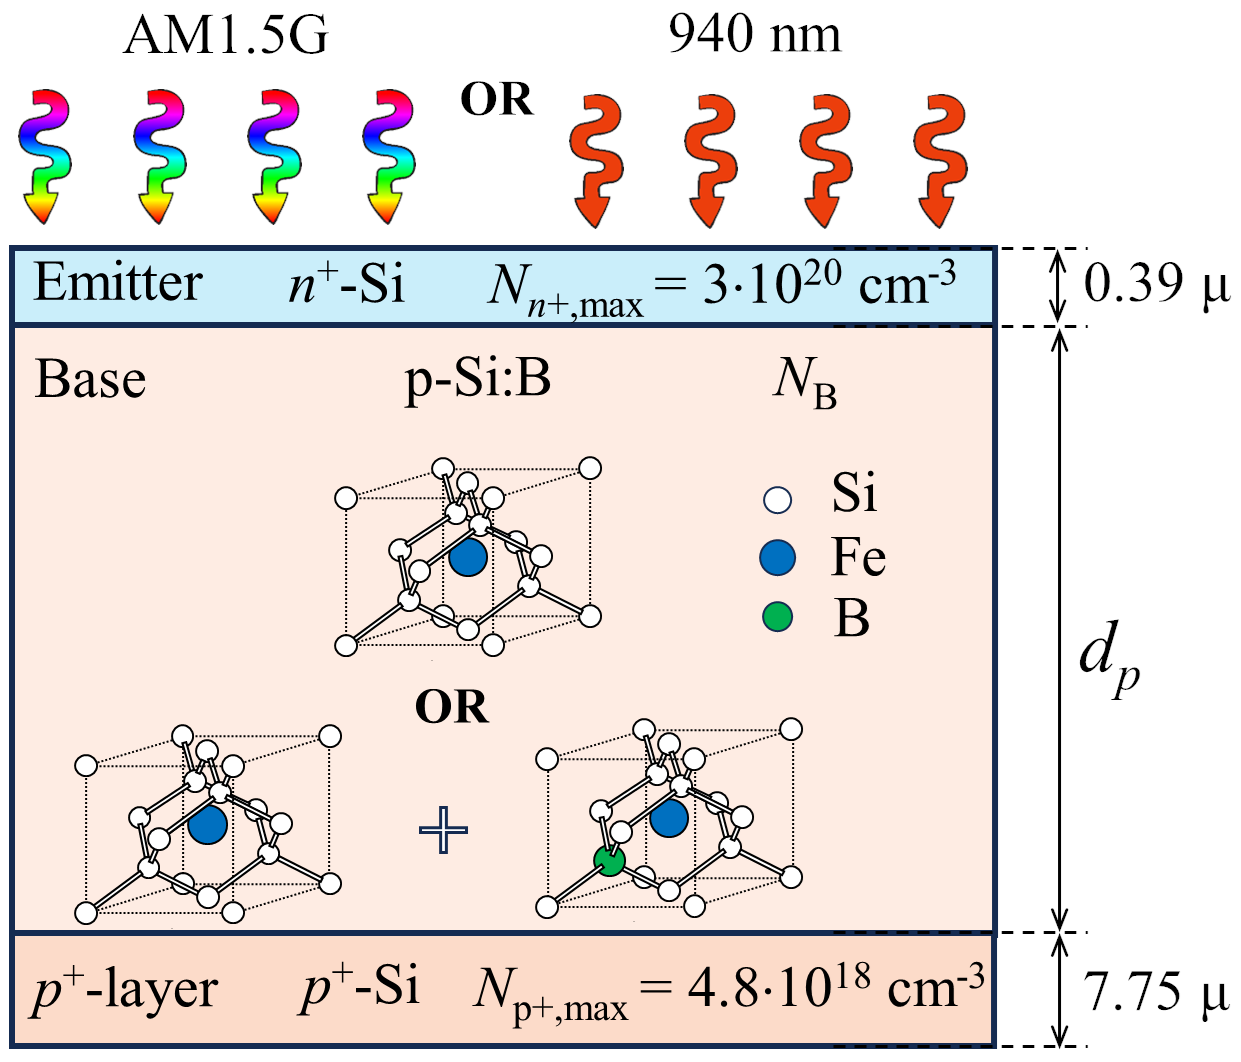
\includegraphics[width=0.5\linewidth]{Figure1.png}
	  \caption{Schematic diagram of analyzed solar cells.}\label{fig1}
\end{figure}


\begin{table}
\caption{Parameters varied during the simulation}\label{table1}
\begin{tabular*}{\tblwidth}{@{}LL@{}}
\toprule
  Parameter & Range of values \\ % Table header row
\midrule
 $d_p$($\mu$m)   & $180-380$\\
 $N_\mathrm{B}$ (cm$^{-3}$)    & $10^{15} - 10^{17}$\\
 $N_\mathrm{Fe}$ (cm$^{-3}$) & $10^{10} - 10^{14}$\\
 $T$ (K)                        & $290 - 340$\\
 Illumination                 & AM1.5G, 1000~W/$\mathrm{m}^{2}$; \\
 & 940~$\mathrm{nm}$, 5~W/$\mathrm{m}^{2}$; 940~$\mathrm{nm}$, 10~W/$\mathrm{m}^{2}$\\
\bottomrule
\end{tabular*}
\end{table}


The simulation was conducted using the SCAPS~3.3.11 code \cite{SCAPS1}.
SCAPS-1D software, developed by the University of Gent, is founded on theoretical computations that involve solving Poisson's equation,
continuity equations for holes and electrons, and drift-diffusion at each position within the solar cell,
considering the boundary conditions.
Despite its one-dimensional modeling approach, SCAPS is extensively used for modeling various types of solar cells \cite{Joshi2024,Ravidas2024,Liu2024,You2023} in general
and for investigating the effects of defects on their performance \cite{AitAbdelkadir2023,Liang2024,SCAPSDefect3} in particular.


As can be seen from Table~\ref{table1}, calculations spanned a broad range of temperatures and base doping levels.
Therefore, to improve the accuracy of the calculations when inputting the initial parameters into SCAPS,
temperature and concentration (where applicable) dependencies of the following silicon parameters were taken into account:

\begin{itemize}
    \item bandgap according to Passler \cite{Passler2002};
    \item doping induced bandgap narrowing according to Yan \& Cuevas \cite{EgNarrow};
    \item effective density of states at conduction and valence band and intrinsic carrier concentration according to Couderc et al. \cite{Si_ni_Couderc};
    \item thermal carrier velocities according to Green \cite{Nc:Green};
    \item free carrier effective masses according to O’Mara et al. \cite{OMara};
    \item carrier mobilities according to Klaassen's theory \cite{KLAASSEN953};
\end{itemize}

The values of surface recombination coefficients were considered equal to the thermal velocities of carriers \cite{Fell2015}.
The calculations addressed recombination processes within the structural volume,
incorporating both intrinsic recombination and Shockley-Read-Hall recombination at iron-related defects.
In the first case, processes of band-to-band radiation recombination were considered
(where the calculation of the corresponding coefficient included the fraction of radiatively emitted photons
reabsorbed via band-to-band processes according to Niewelt et al.\cite{Brad2022})
and Auger recombination (where the coefficients considered the effect of Coulomb enhancement \cite{AugerSi2022} and temperature dependence \cite{Si_Auger}).


When accounting for the influence of iron impurities,
we considered that Fe atoms were uniformly distributed within the base and $p^+$-layer
with a total concentration of $N_\mathrm{Fe}$ (see Table~\ref{table1}).
Two cases were under consideration:

Case~1.
The concentration of interstitial iron defects $\left[\mathrm{Fe}_i\right]=N_\mathrm{Fe}$  at each position throughout the solar cell,
with no pairs present $\left[\mathrm{Fe}_i\mathrm{B}_s\right]=0$.
This case corresponds to the state of the structure immediately after intense illumination, for example.

Case~2.
Iron atoms predominantly form pairs with acceptors, $\left[\mathrm{Fe}_i\mathrm{B}_s\right] \gg \left[\mathrm{Fe}_i\right]$,
but the exact concentration ratio depends on the position of the Fermi level and temperature \cite{FeB:kinetic,MurphyJAP2011}
and varies from point to point within the solar cell.
Further details about calculation of the concentration profiles of Fe$_i$B$_s$ and Fe$_i$ are provided in \cite{Olikh2022PPV,Olikh2019SM}.
This case corresponds to prolonged storage of the structure in darkness or under conditions of low-intensity ($< 0.01$~J~cm$^{-2}$ \cite{Macdonald2004}) illumination.


During the calculations, it was assumed that Fe$_i$ forms a single donor level,
while the Fe$_i$B$_s$ pair has a trigonal configuration and acts as an amphoteric defect.
We obtained defect parameters (including level positions within the bandgap and electron and hole capture cross-sections) from relevant studies \cite{ROUGIEUX2018,Istratov1999,Paudyal}.

As previously mentioned, the solar cell behavior was simulated under different illumination conditions,
including solar light (AM1.5G) and monochromatic light (wavelength 940~nm, intensity of $W_\mathrm{ill} = 5$~Wm$^{-2}$ or 10~W/$\mathrm{m}^{2}$) --– see Table~\ref{table1}.
The calculations incorporated the light absorption values in silicon based on Green's study \cite{Green2022}.


The $I$-$V$ characteristics were simulated for both Case~1 and Case~2 (see Fig.~\ref{fig2}),
and from each curve, the short-circuit current, open-circuit voltage, efficiency, and fill factor were determined.
Assessing the influence of iron defect variability relied on the relative changes in each photovoltaic conversion parameter:

\begin{figure}
	\centering
		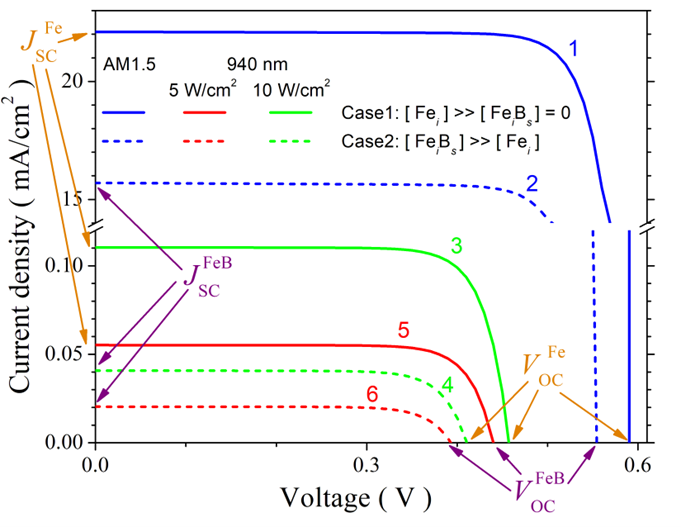
\includegraphics[width=0.5\linewidth]{Figure2.png}
	  \caption{Typical IV characteristics,
   calculated for structure with $d_p = 180$~$\mu$m, $N_\mathrm{B}=10^{17}$~cm$^{-3}$,
   $N_\mathrm{Fe}=10^{14}$~cm$^{-3}$ at $T = 290$~K.
   Illumination: AM1.5 (curves 1, 2), 940~nm 10~Wcm$^{-2}$ (3, 4) and 940~nm 5~Wcm$^{-2}$ (5, 6).
   Solid and dotted lines correspond to Case~1 and Case~2, respectively.}\label{fig2}
\end{figure}


\begin{equation}
\label{eq1}
    \varepsilon A = \frac{A^\mathrm{FeB} - A^\mathrm{Fe}}{A^\mathrm{FeB}} \times 100 \%\,,
\end{equation}
where $A$ represents one of the parameters ($I_\mathrm{SC}$, $V_\mathrm{OC}$, $\eta$, and $F\!F$),
superscript ‘‘FeB’’ corresponds to the parameter value for coexistence of Fe$_i$ and Fe$_i$B$_s$ (Case~2),
superscript ‘‘Fe’’ is related to the decay of all pairs (Case~1).


Impact of change of iron defects was investigated as a function of temperature from 290~K to 340~K,
base depth from 180~$\mu$m to 380~$\mu$m,
base doping level from $10^{15}$~cm$^{-3}$ to $10^{17}$~cm$^{-3}$,
and total impurity iron atom concentration from $10^{10}$~cm$^{-3}$ to $10^{14}$~cm$^{-3}$.
For each illumination scenario, calculations were carried out with 11 different temperature values and 5 base depth values,
evenly distributed within the specified ranges.
The concentration values were distributed equally on a logarithmic scale with 4 ($N_\mathrm{B}$ case) and 6 ($N_\mathrm{Fe}$ case) steps per decade.
As a result, for the AM1.5 illumination scenario, for instance, 24750 $I$-$V$ characteristics were simulated.
An exception occurred with monochromatic illumination at $W_\mathrm{ill} = 10$~Wm$^{-2}$,
where we used only two $d_p$ values.

\subsection{Experimental Details}

To evaluate the validity of the simulated results,
we also conducted experimental studies on the effect of changing the state of iron-related defects on the photoelectric parameters of silicon solar cells.

The $n^+$-$p$-$p^+$-Si samples were used in the experiment.
The structure was fabricated from a 380~$\mu$m thick $p$-type boron-doped
Czochralski silicon (100) wafer with doping level $N_\mathrm{B}=1.36\times10^{15}$~cm$^{-3}$.
The $n^+$ emitter with a sheet resistance of about $20-30$~$\Omega/\Box$
and  thickness of $0.7$~$\mu$m was formed by phosphorus diffusion.
The anti-recombination isotype barrier was created by using a $p^+$
layer ($10-20$~$\Omega/\Box$) formed by boron diffusion.
On the front surface, SiO$_2$ (40~nm) and Si$_3$N$_4$ (30~nm) films were formed as antireflective and passivating layers, respectively.
The solid and grid Al contacts were formed by magnetron sputtering on the back and front surfaces, respectively.

The $I$-$V$ characteristics were measured using a Keithley 2450 source meter and
low--intensity monochromatic light source (light--emitting diode SN--HPIR940nm--1W with light wavelength 940~nm and intensity of about  $W_\mathrm{ill} = 5$~Wm$^{-2}$).

For different samples, the iron concentration ranged from $2\times10^{11}$ to $4\times10^{13}$~cm$^{-3}$.
The values of $N_\mathrm{Fe}$ were determined using a methodology \cite{Olikh2022:JMatSci,Olikh2021JAP}, based on fitting the kinetics of short-circuit current.
The decay of Fe$_i$B$_s$ pairs was realized using intensive (7000~W/$\mathrm{m}^{2}$) halogen lamp illumination.

The measurements were carried over the temperature range of 300-340~K.
The sample temperature was driven by a thermoelectric cooler controlled by an STS-21 sensor
and maintained constant by a PID algorithm embedded in the software that serves the experimental setup.


\section{Results and Discussion}%\label{}

\subsection{Short--circuit current}

Figure~\ref{fig3} illustrates the characteristic dependencies of short-circuit current variations resulting
from the reconfiguration of iron-containing defects, as obtained from the simulations.
We present a more comprehensive set of figures that depict the detailed dependencies of $\varepsilon I_\mathrm{SC}$ on
all parameters varied during the calculations in the Supplementary Material (Figs.~S1-S6).
It is important to note that the qualitative nature of the short-circuit current variations remains practically identical
under both solar and monochromatic illumination, with the quantitative parameters of $\varepsilon I_\mathrm{SC}$ differing:
at 940~nm, the absolute values of $\varepsilon I_\mathrm{SC}$ are approximately 3--4 times greater than those observed under AM1.5 conditions,
assuming other parameters are constant.
Among other features of $\varepsilon I_\mathrm{SC}$ changes, we can highlight the following:


\begin{figure}
	\centering
     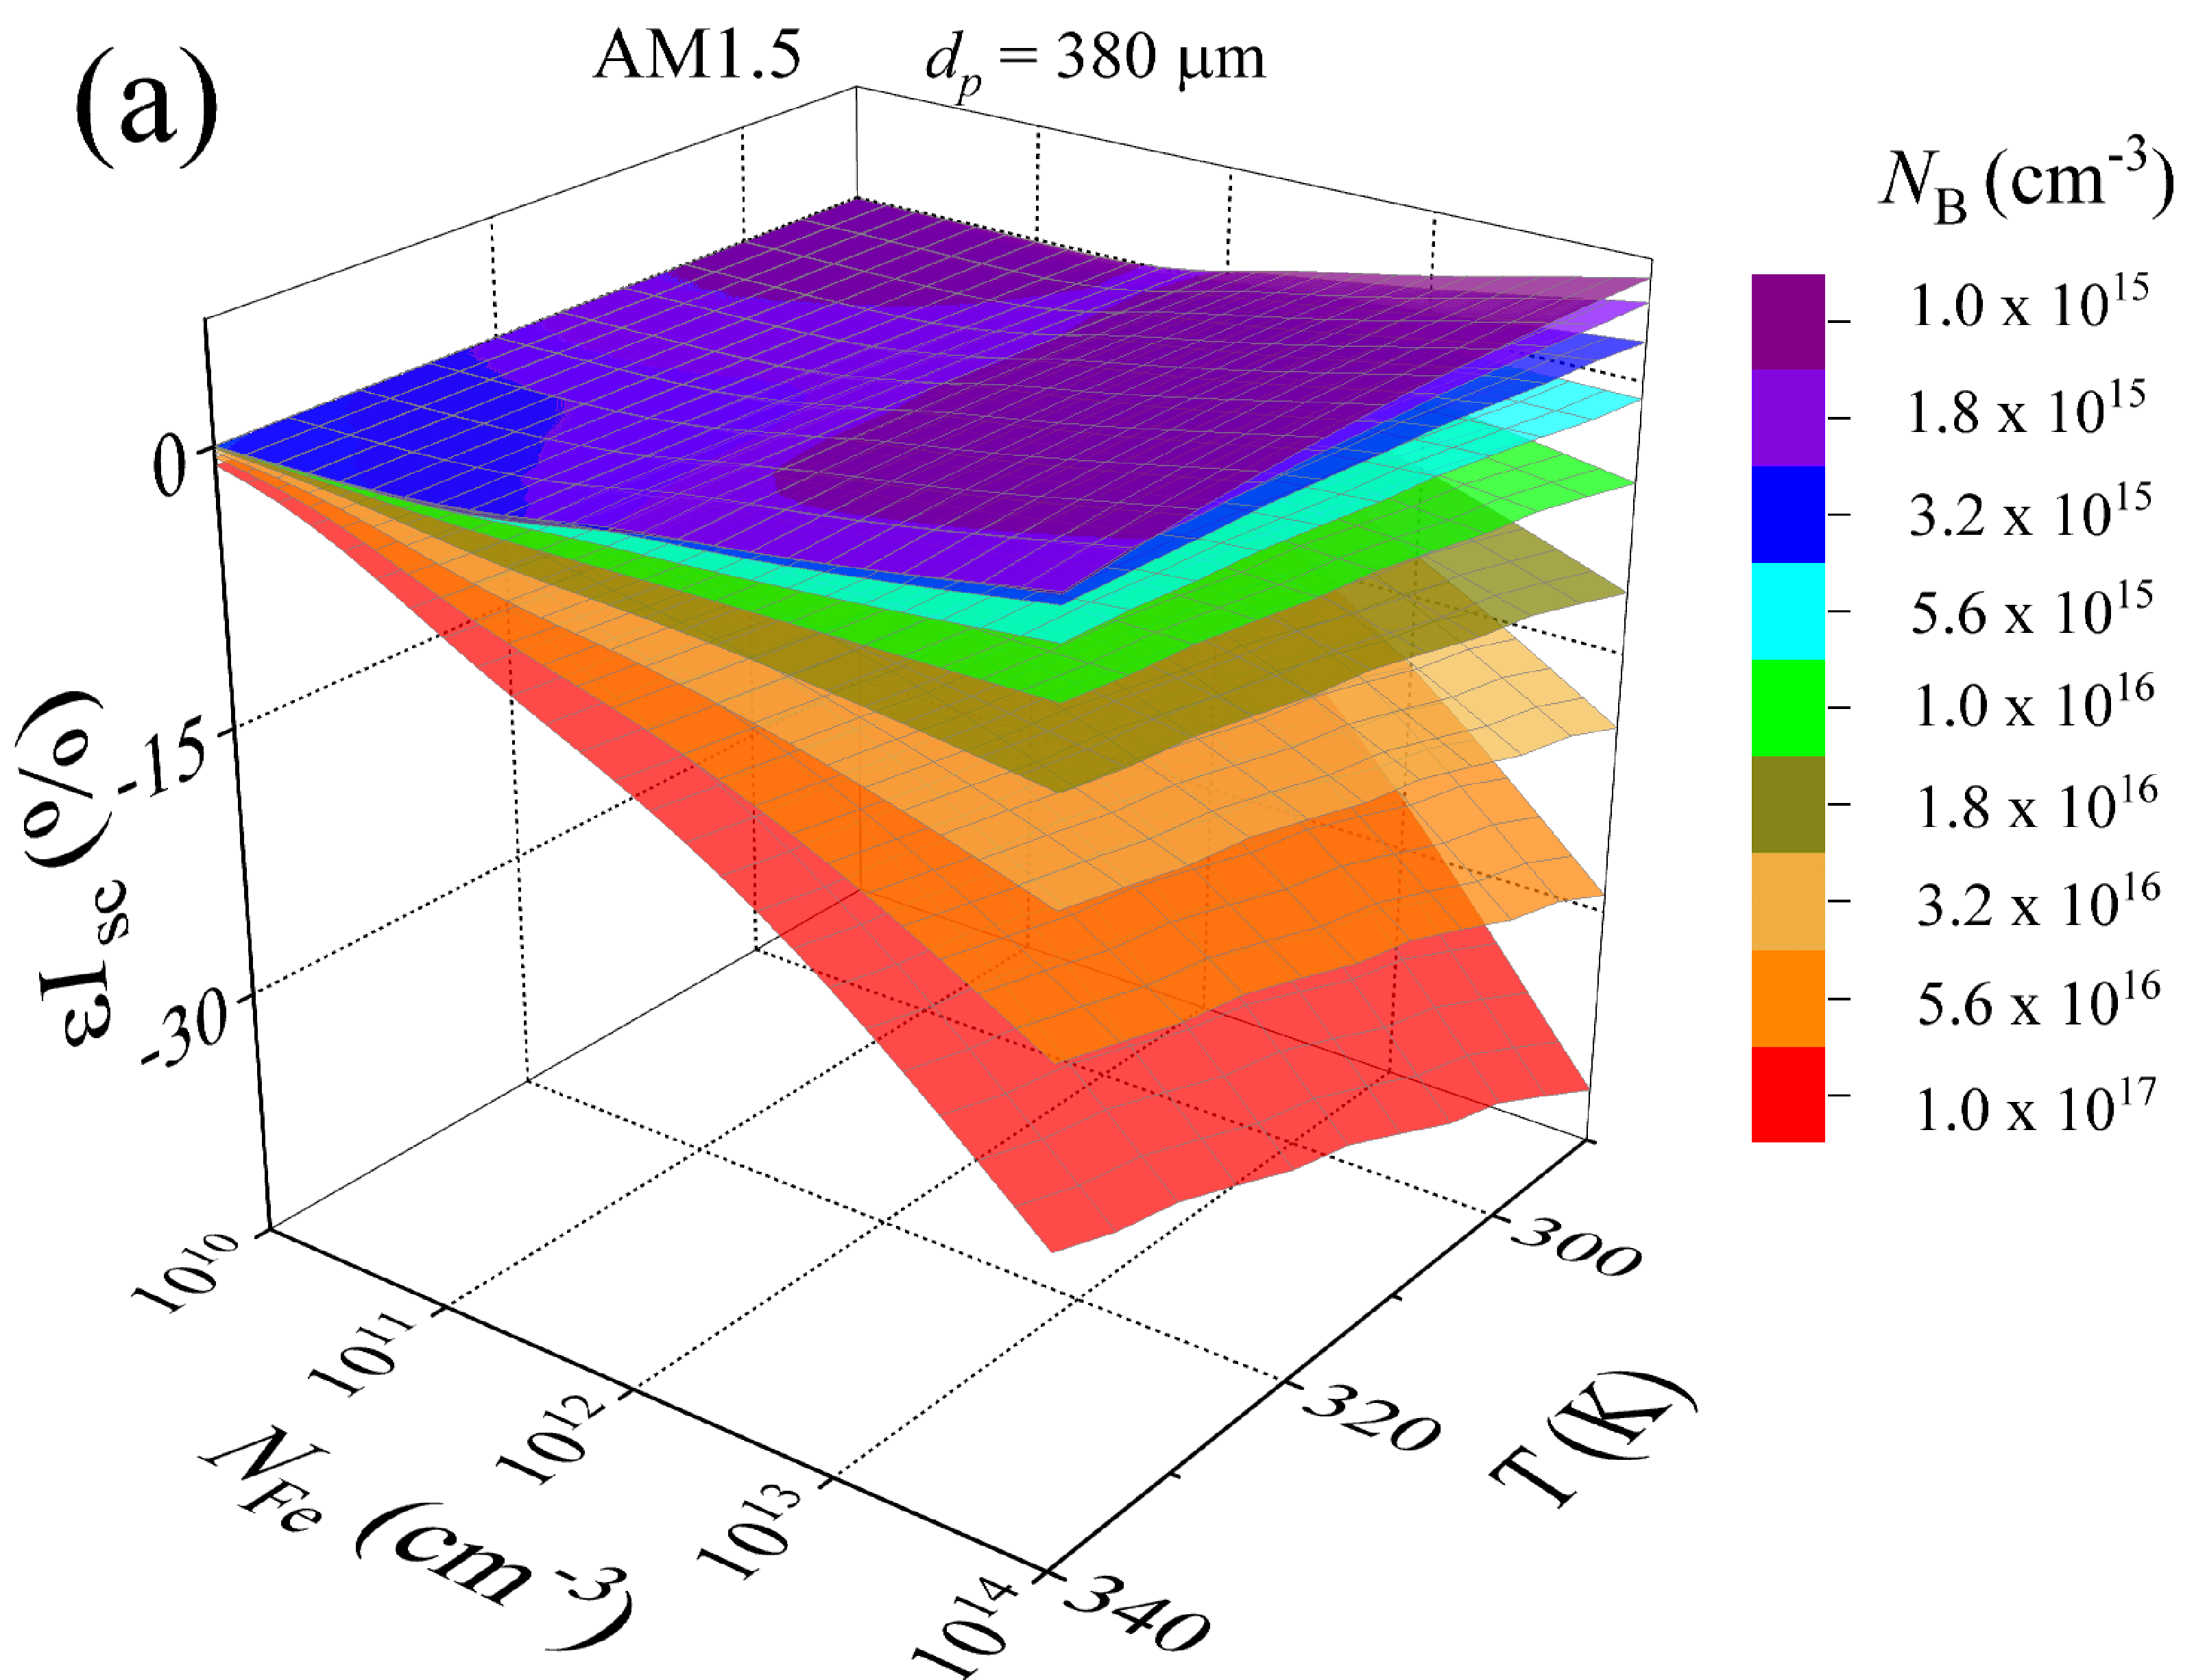
\includegraphics[width=0.49\linewidth]{Fig3a.png}
     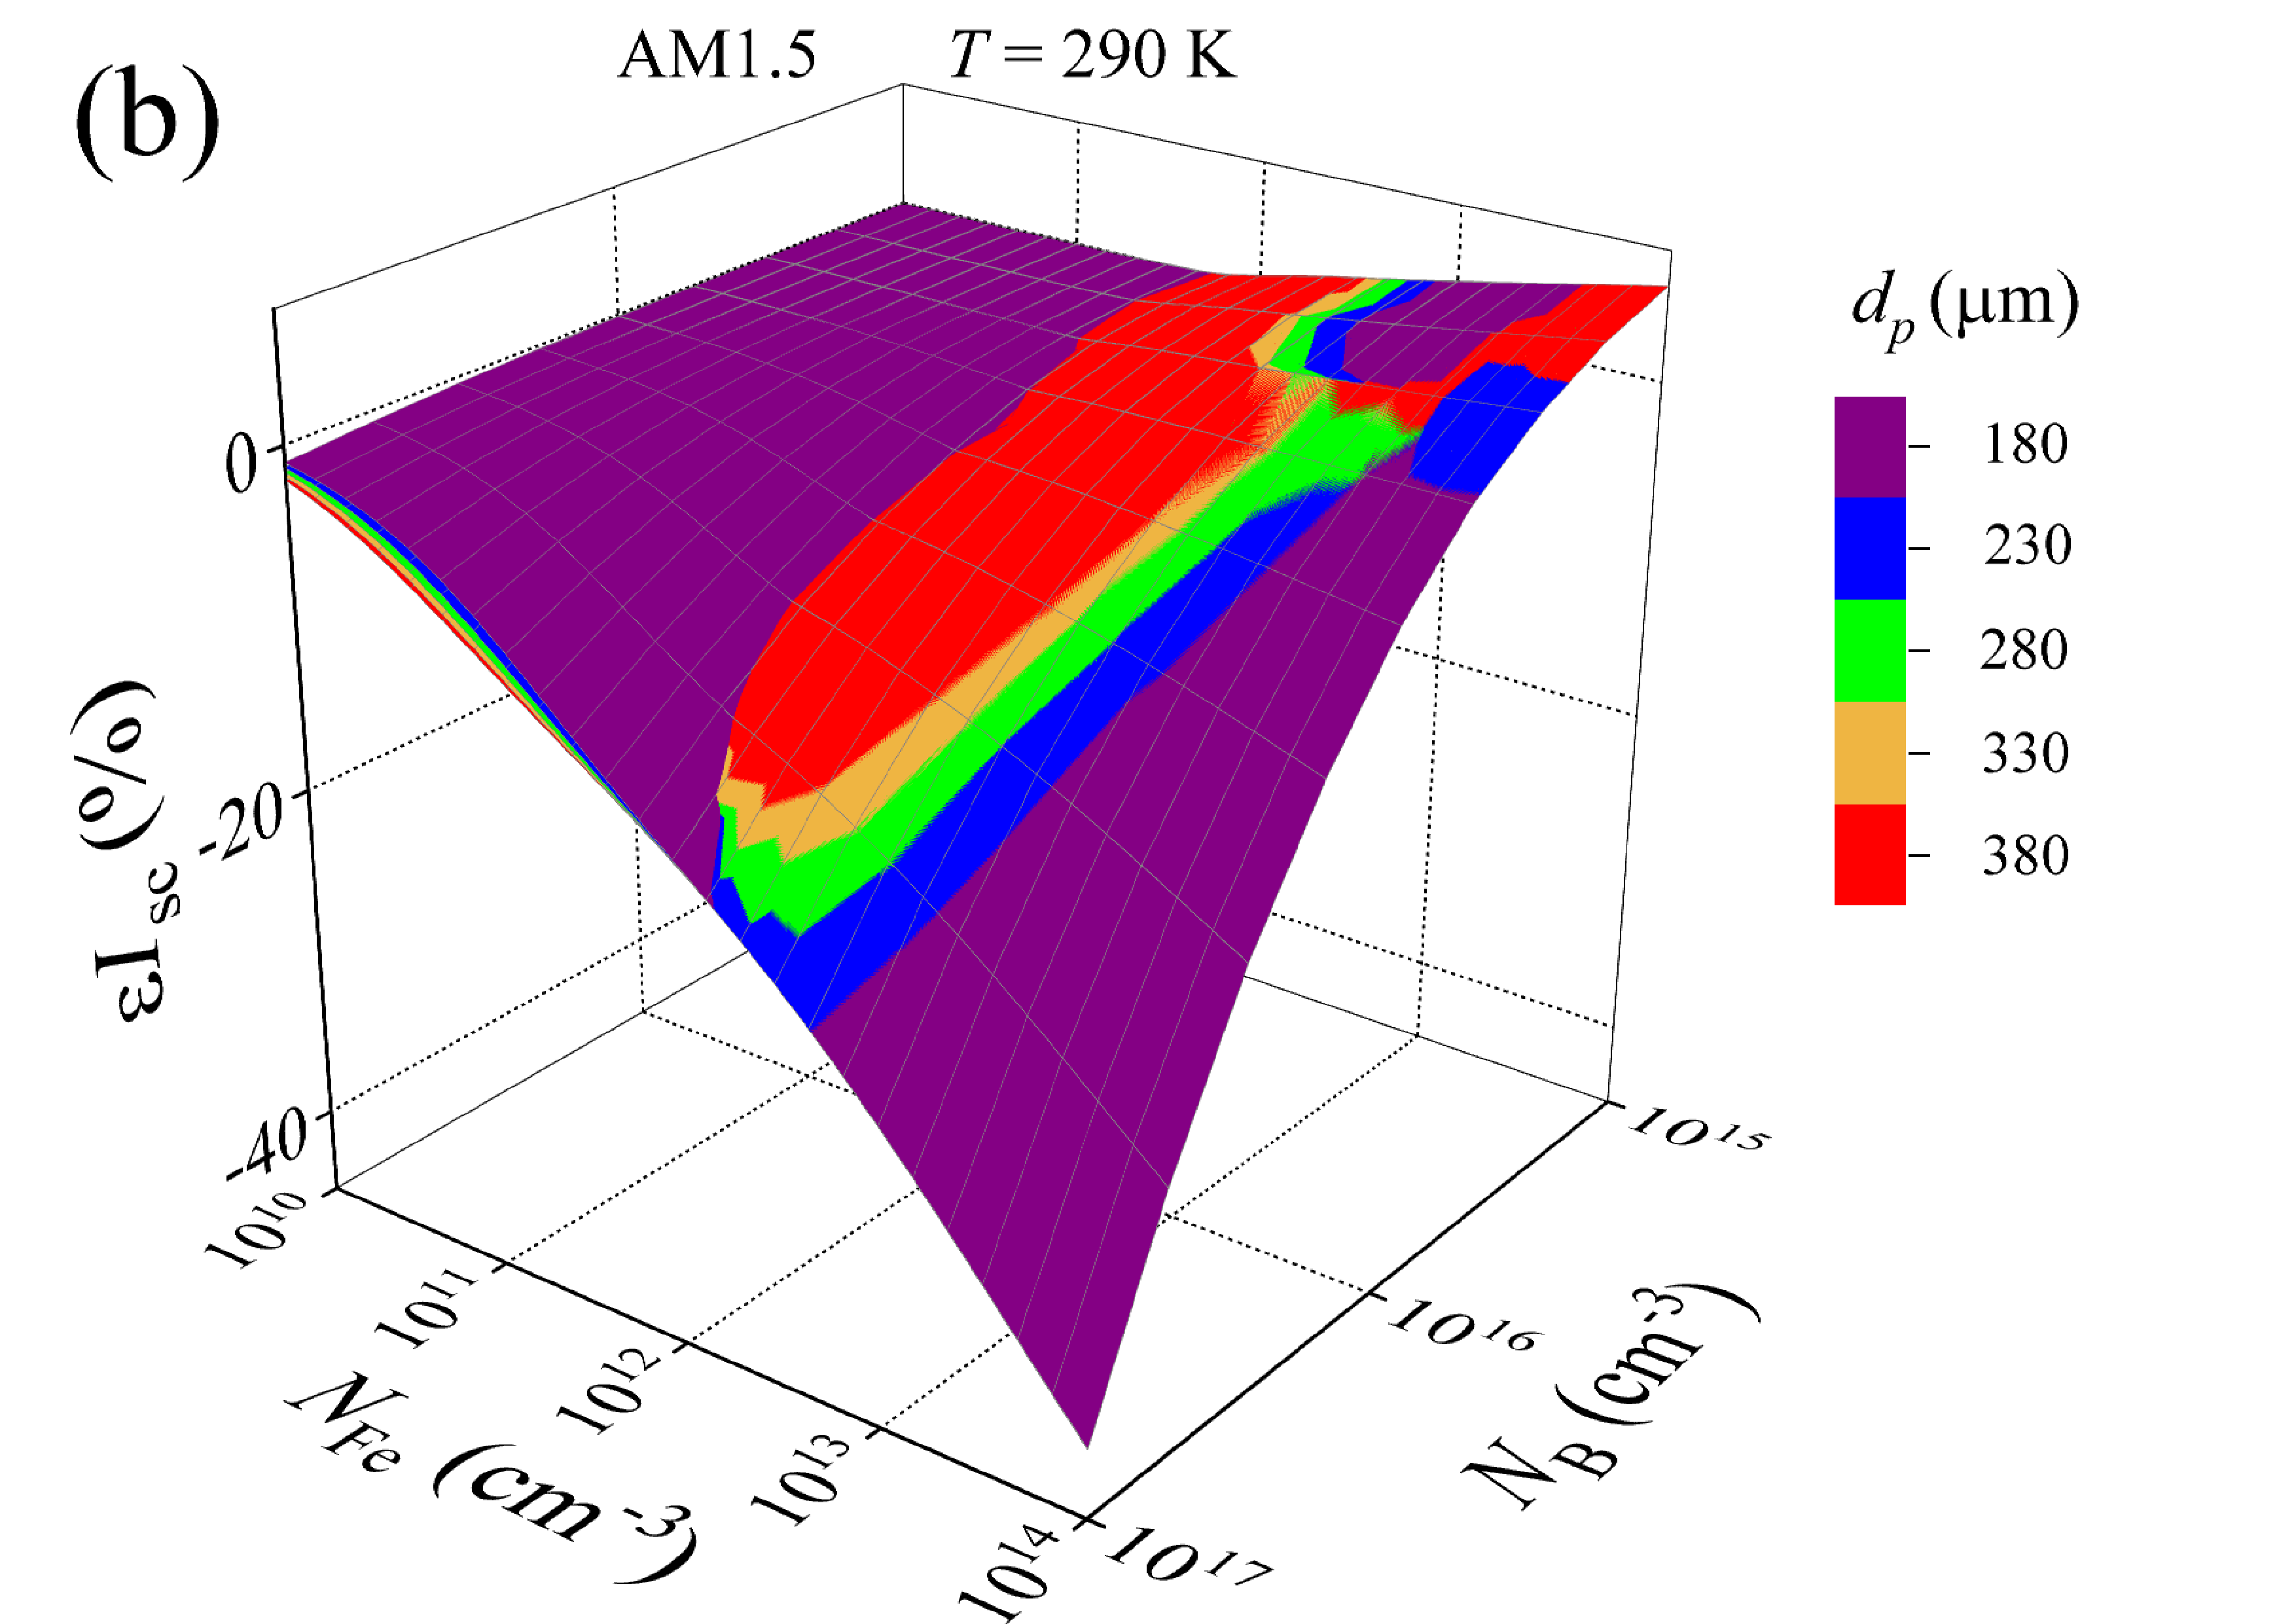
\includegraphics[width=0.49\linewidth]{Fig3b.png}
     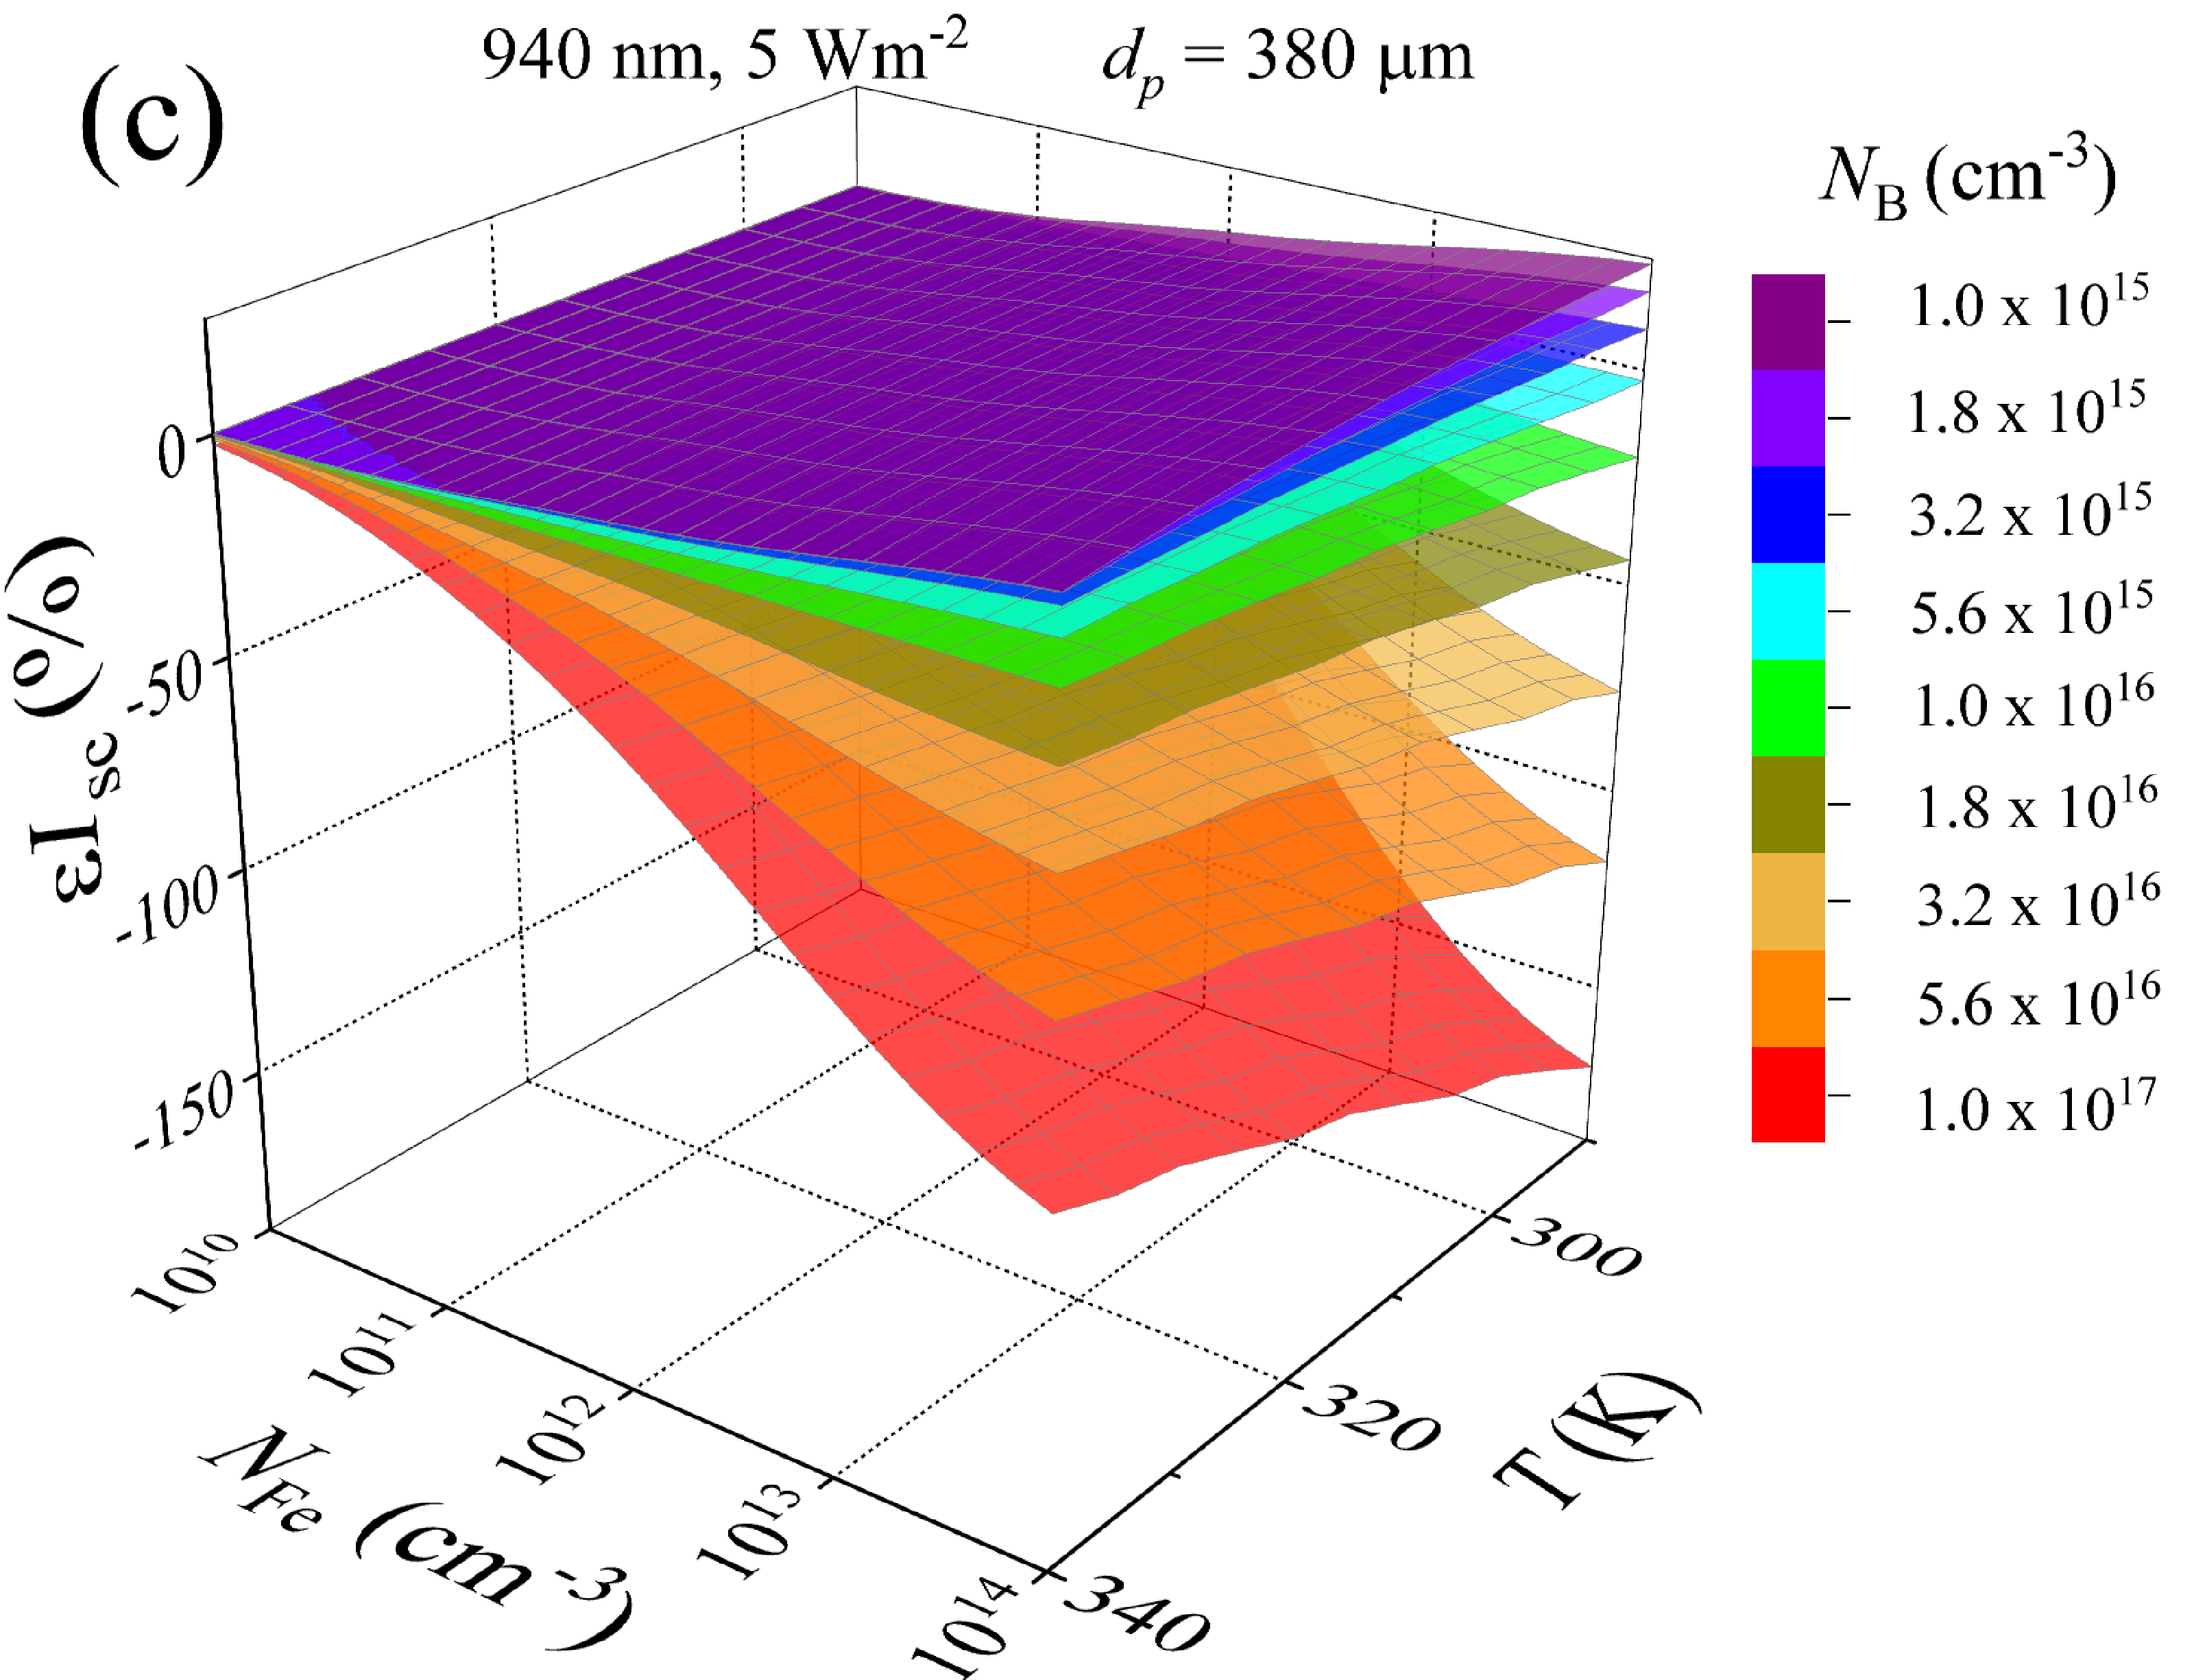
\includegraphics[width=0.49\linewidth]{Fig3c.png}
     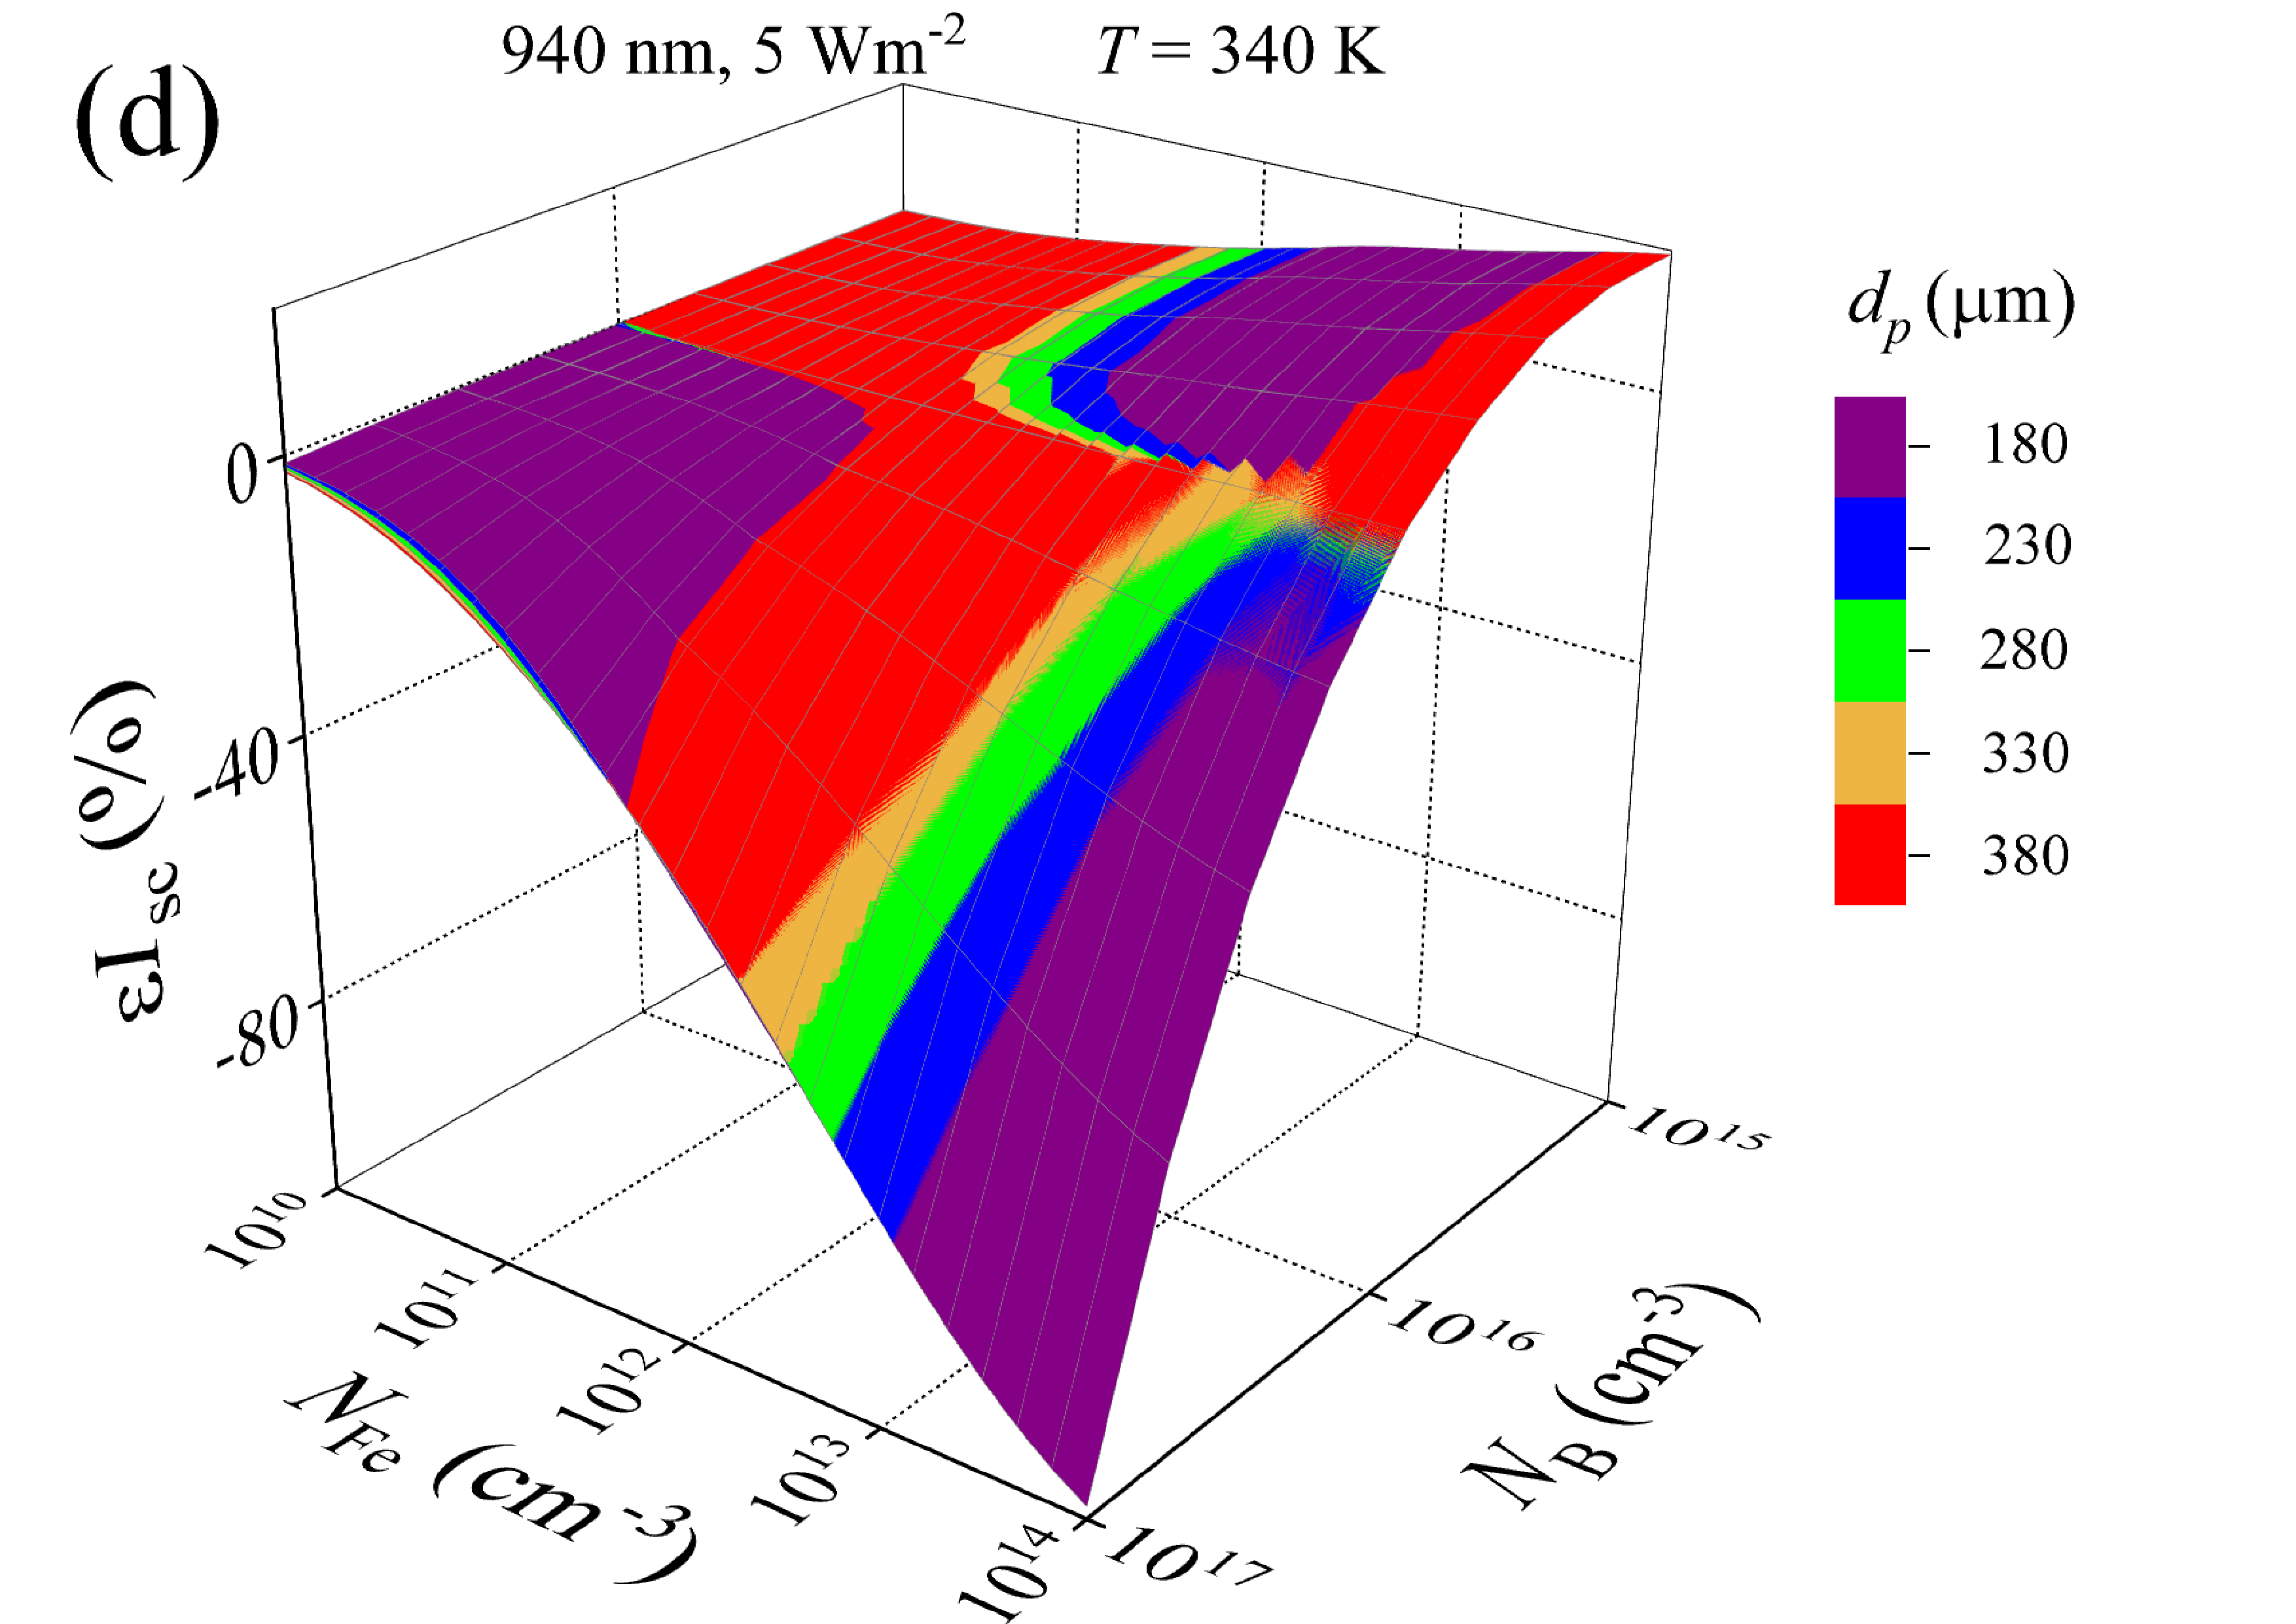
\includegraphics[width=0.49\linewidth]{Fig3d.png}
	  \caption{Relative changes in short-circuit current caused by a complete
       dissociation of Fe$_i$B$_s$ pairs as a function of
       iron concentration and
       temperature (panels a and c) or doping level (b, d).
       Illumination: AM1.5 (a, b), 940~nm 5~Wm$^{-2}$ (c, d).
       $T$, K: 290 (b), 340 (d).
       Different surfaces correspond to different doping levels (a, c) and base depths (b, d).
}\label{fig3}
\end{figure}

\noindent
- The module $\varepsilon I_\mathrm{SC}$ increases monotonically with increasing iron concentration,
    but the sign of this value depends on the doping level.
    At low boron concentrations ($N_\mathrm{B}=10^{15}$~cm$^{-3}$) $\varepsilon I_\mathrm{SC} > 0$,
    whereas at high concentrations ($N_\mathrm{B}=10^{17}$~cm$^{-3}$) $\varepsilon I_\mathrm{SC} < 0$ - see Figs.~\ref{fig3}a,~\ref{fig3}c, S3--S6;

\noindent
- Increasing the acceptor concentration causes a monotonic decrease in $\varepsilon I_\mathrm{SC}$ (Figs.~\ref{fig3}b,~\ref{fig3}d);
    the $N_\mathrm{B}$ value at which the sign of $\varepsilon I_\mathrm{SC}$ changes depends on the temperature
    (decreases with decreasing in $T$ value) and the type of illumination (is generally higher in the case of monochromatic light) --- see Fig.~S2;

\noindent
 - In the case where $\varepsilon I_\mathrm{SC} < 0$, an temperature increase causes a decrease in the absolute magnitude
    of the relative changes in short--circuit current, with the dependence being nearly linear and
    the slope increasing with higher doping levels and iron concentration (Figs.~\ref{fig3}a,~\ref{fig3}c, S4).
    In the case where $\varepsilon I_\mathrm{SC} > 0$,
    a $T$ changing results in minor non-monotonic variations of the short-circuit current after the dissociation of Fe$_i$B$_s$  pairs (Fig.~S3);

\noindent
- The influence of base thickness on $\varepsilon I_\mathrm{SC}$ increases with
    increasing $N_\mathrm{B}$ and decreasing $N_\mathrm{Fe}$ (Figs.~S5, S3), but it is minimal overall.
    As calculations have shown, increasing $d_p$ by more than twice causes changes in $\varepsilon I_\mathrm{SC}$ that do not exceed 0.5~\%;

\noindent
- Changing the intensity of the monochromatic illumination (from 5~W/m$^{2}$ to 10~W/m$^{2}$) does not practically change the value of $\varepsilon I_\mathrm{SC}$;


\noindent
- The absolute values of $\varepsilon I_\mathrm{SC}$ can reach relatively high values (more than 100~\% for 940~nm illumination);
    however, in cases where $N_\mathrm{Fe}<10^{11}$~cm$^{-3}$ and around $N_\mathrm{B}=10^{16}$~cm$^{-3}$, the changes in short-circuit current do not exceed a few percent.



The identified features of the $\varepsilon I_\mathrm{SC}$ changes can be explained by considering
the main reasons for the influence of factors, which varied during simulation, on the photovoltaic conversion.
It is known \cite{YangHandbookPVSi} that the main influence of metal impurities on solar cell performance is caused
by their effect on the collection efficiency (CE, portion of excess carriers that reach the depletion region of $p$–$n$ junction).
Neglecting the influence of series and shunt resistances, the short-circuit current coincides with the photocurrent $I_\mathrm{ph}$,
which equals the CE multiplied by the number of light-induced excess carriers.
In turn, the CE can be calculated as a convolution of generation function, which is proportional to $\exp(-\alpha z)$
(where $\alpha$ is the absorption coefficient and $z$ is the coordinate along the axis directed
perpendicular to the $p$-$n$ junction from the emitter)
and the collection probability, which can be obtained as a solution of homogeneous diffusion equation.

The photogenerated current for the cell can be obtained by adding the relevant quantities
for the base $I_\mathrm{ph,b}$ and the emitter $I_\mathrm{ph,e}$ \cite{Markvart}:
\begin{equation}
\label{eq2}
     I_\mathrm{SC} \approx I_\mathrm{ph} = I_\mathrm{ph,e} + I_\mathrm{ph,b}\,.
\end{equation}


However, considering the location of the impurity iron,
it can be assumed that during the Fe$_i$B$_\mathrm{Si}$ $\rightleftharpoons$ Fe$_i$ + B$_\mathrm{Si}$ reconfiguration,
the first term on the right-hand side of Eq.~(\ref{eq2})
remains unchanged ($I_\mathrm{ph,e}^\mathrm{FeB}$ = $I_\mathrm{ph,e}^\mathrm{Fe}$ = $I_\mathrm{ph,e}$),
and therefore, considering Eq.~(\ref{eq1}):
\begin{equation}
\label{eq3}
     \varepsilon I_\mathrm{SC} = \frac{I_\mathrm{ph,b}^\mathrm{FeB}-I_\mathrm{ph,b}^\mathrm{Fe}}{I_\mathrm{ph,e}+I_\mathrm{ph,b}^\mathrm{FeB}}\times 100 \%\,.
\end{equation}

In turn, the base photocurrent the under monochromatic illumination can be expressed  as follows \cite{Goetzberger1998}:
\begin{equation}
\label{eq4}
     I_\mathrm{ph,b}=\frac{qF(1-R)\alpha L_n}{{\alpha}^2 L_n^2 - 1}\left( \alpha L_n - \frac{\frac{SL_n}{D_n}\left[ {\cosh\left( \frac{d^*}{L_n} \right)} - \exp(-\alpha d^*) \right] + \sinh\left( \frac{d^*}{L_n} \right) + \alpha L_n \exp(-\alpha d^*)}{\frac{SL_n}{D_n}\sinh\left( \frac{d^*}{L_n} \right) + \cosh\left( \frac{d^*}{L_n} \right)} \right)\,,
\end{equation}
where
$F$ is the photon flux,
$R$ is the reflection coefficient,
$S$ is the surface recombination velocity,
$L_n$ is the minority carrier (electron) diffusion length,
$D_n$ is the electron diffusion coefficient,
$d^*$ is the thickness of the quasi-neutral region base,
since the space charge region (SCR) width for the modeled structures did not exceed 1~$\mu$m,
it follows that $d^*\simeq d_p$.

The recombination rate affects the value of $L_n$ and, according to the Shockley--Read--Hall model,
depends on trap concentrations, capture cross-sections of electrons and holes, temperature, the Fermi level $E_\mathrm{F}$ location, and defect levels.
Temperature also affects the values of $\alpha$ and $D_n$.
In turn, the position of $E_\mathrm{F}$ within the band gap depends on temperature and doping level.
Fig.~\ref{fig4} shows the calculated by using SCAPS temperature and concentration dependence of the Fermi level in the base of the investigated structure.
In addition, this figure shows the positions of the levels associated with interstitial iron and the FeB pair.
It is worth noting that Fe$_i$ acts as a deep center;
the donor state of the Fe$_i$B$_s$ pair shows only negligible recombination activity,
while the presence of the acceptor state Fe$_i$B$_s$ causes the
carrier lifetime to be doping-dependent under low injection conditions \cite{FeB:Schmidt}.

\begin{figure}
	\centering
     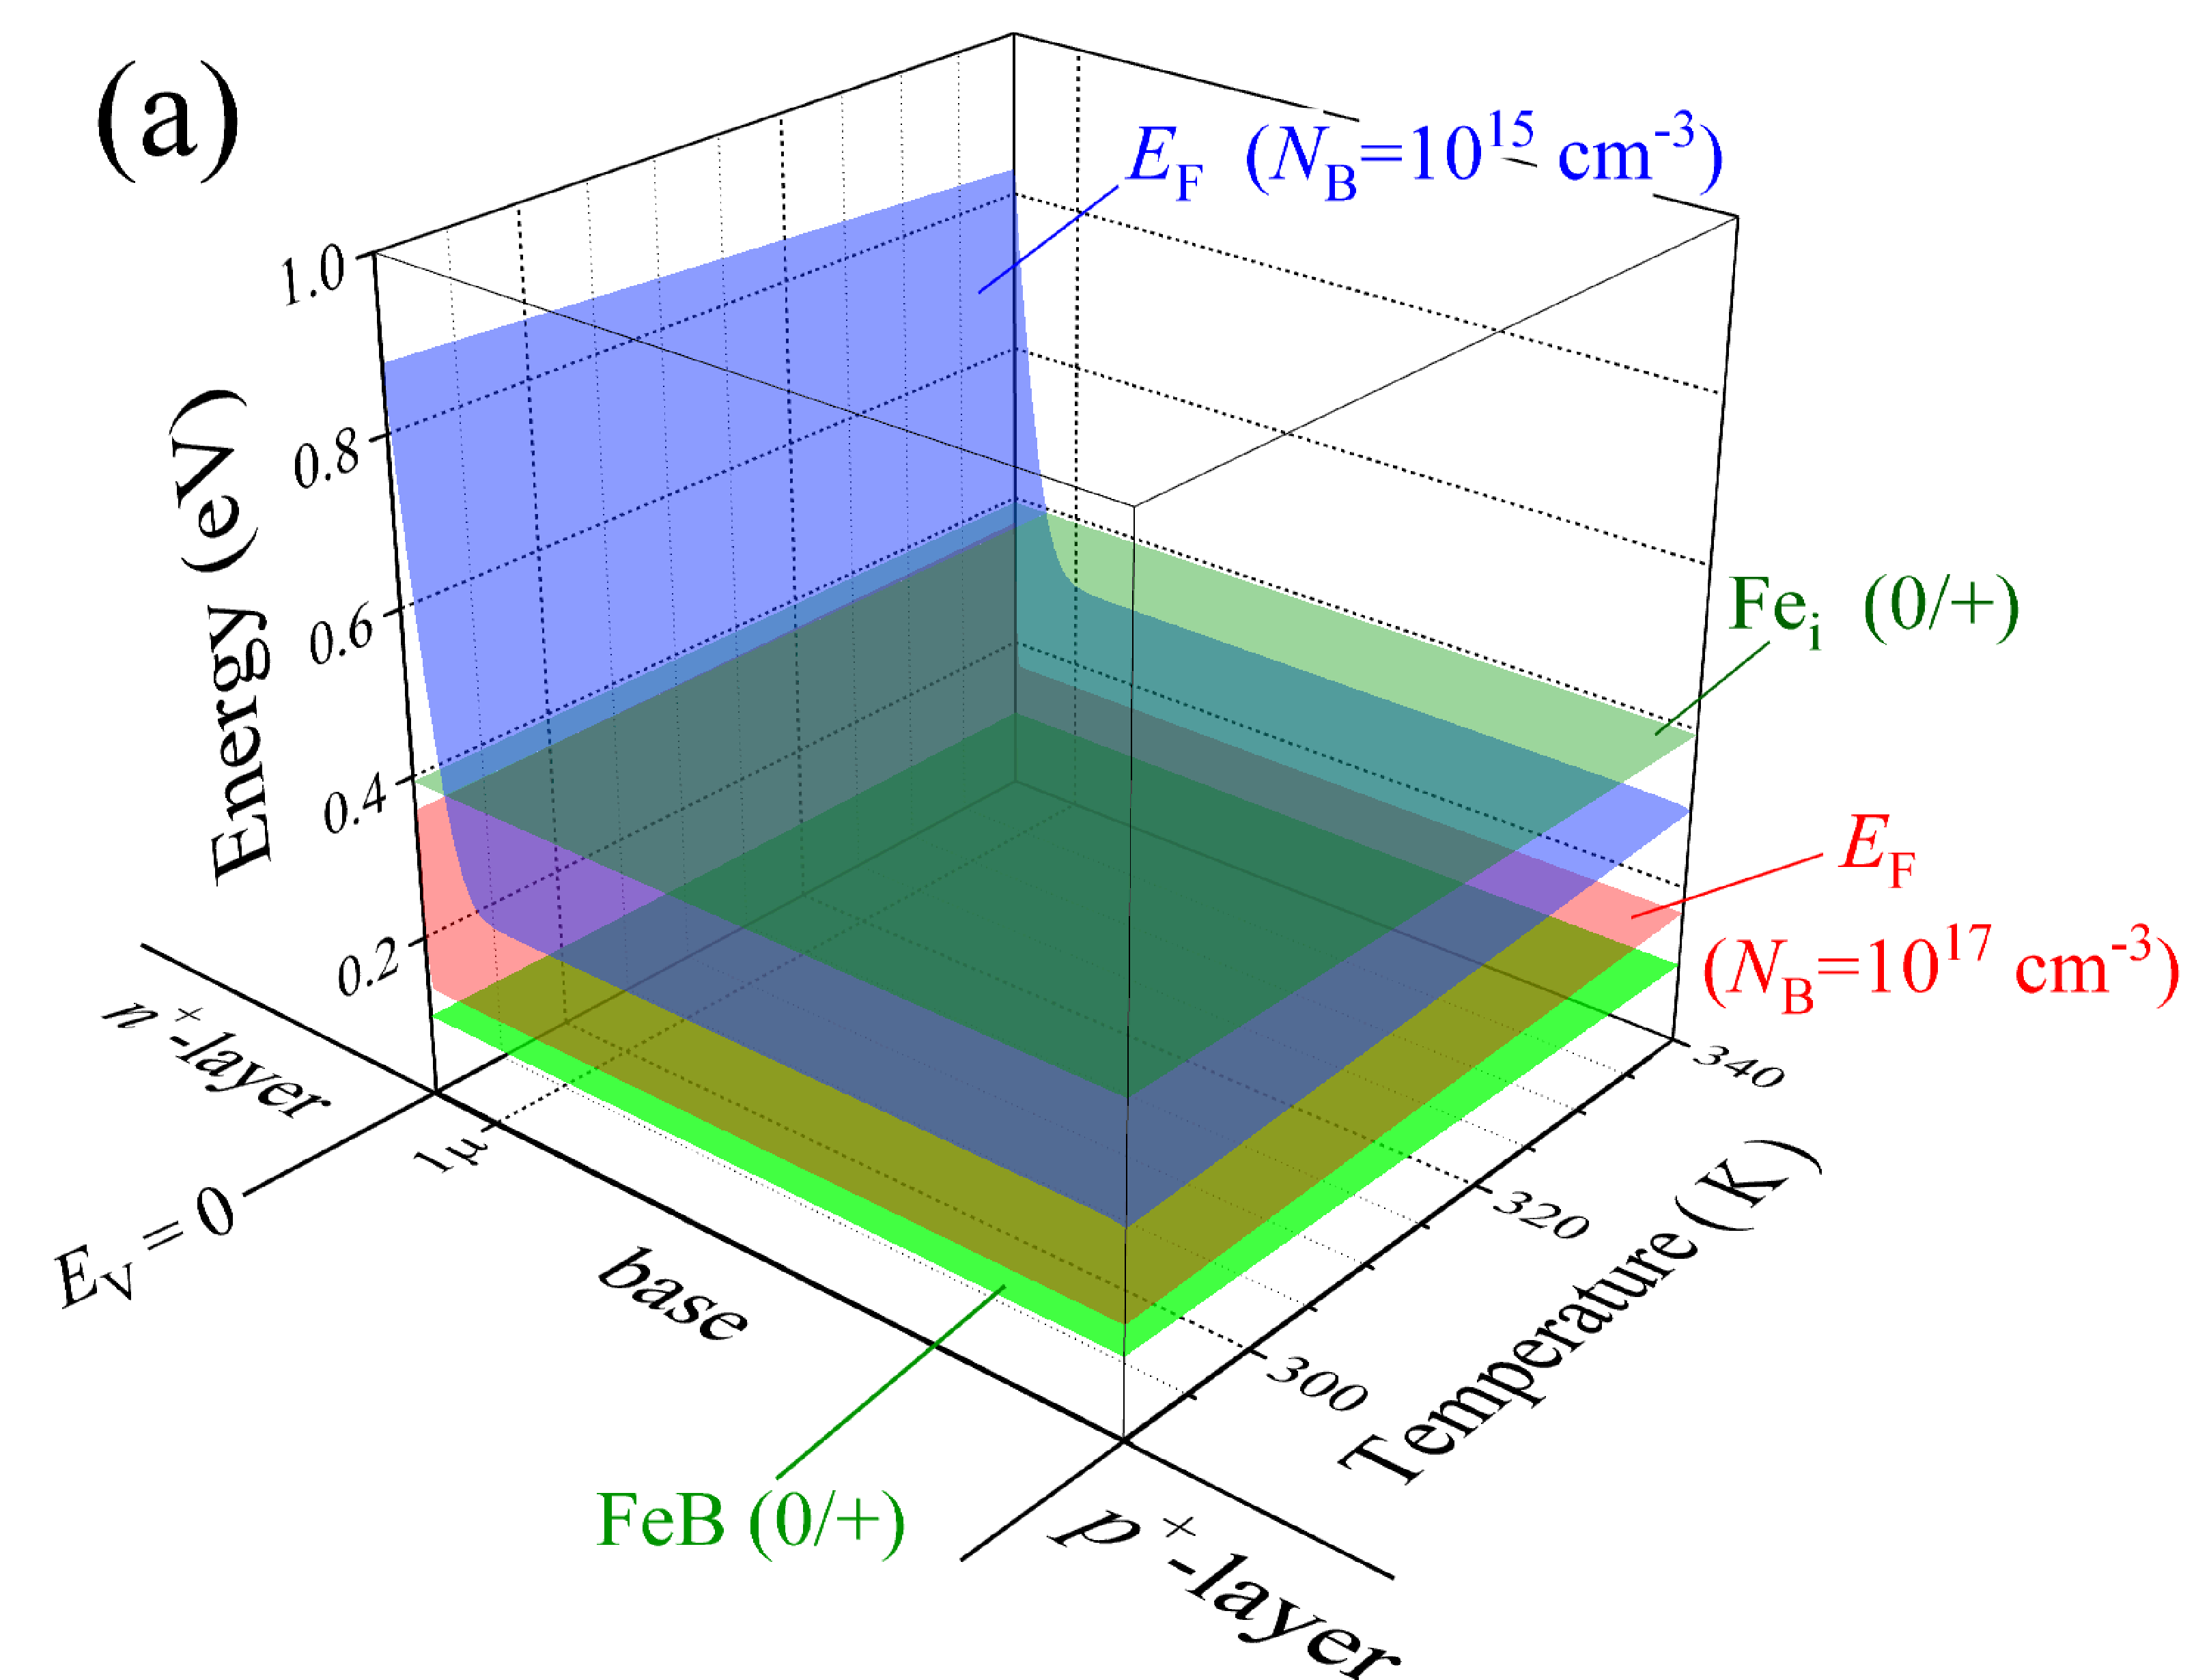
\includegraphics[width=0.49\linewidth]{Fig4a.png}
     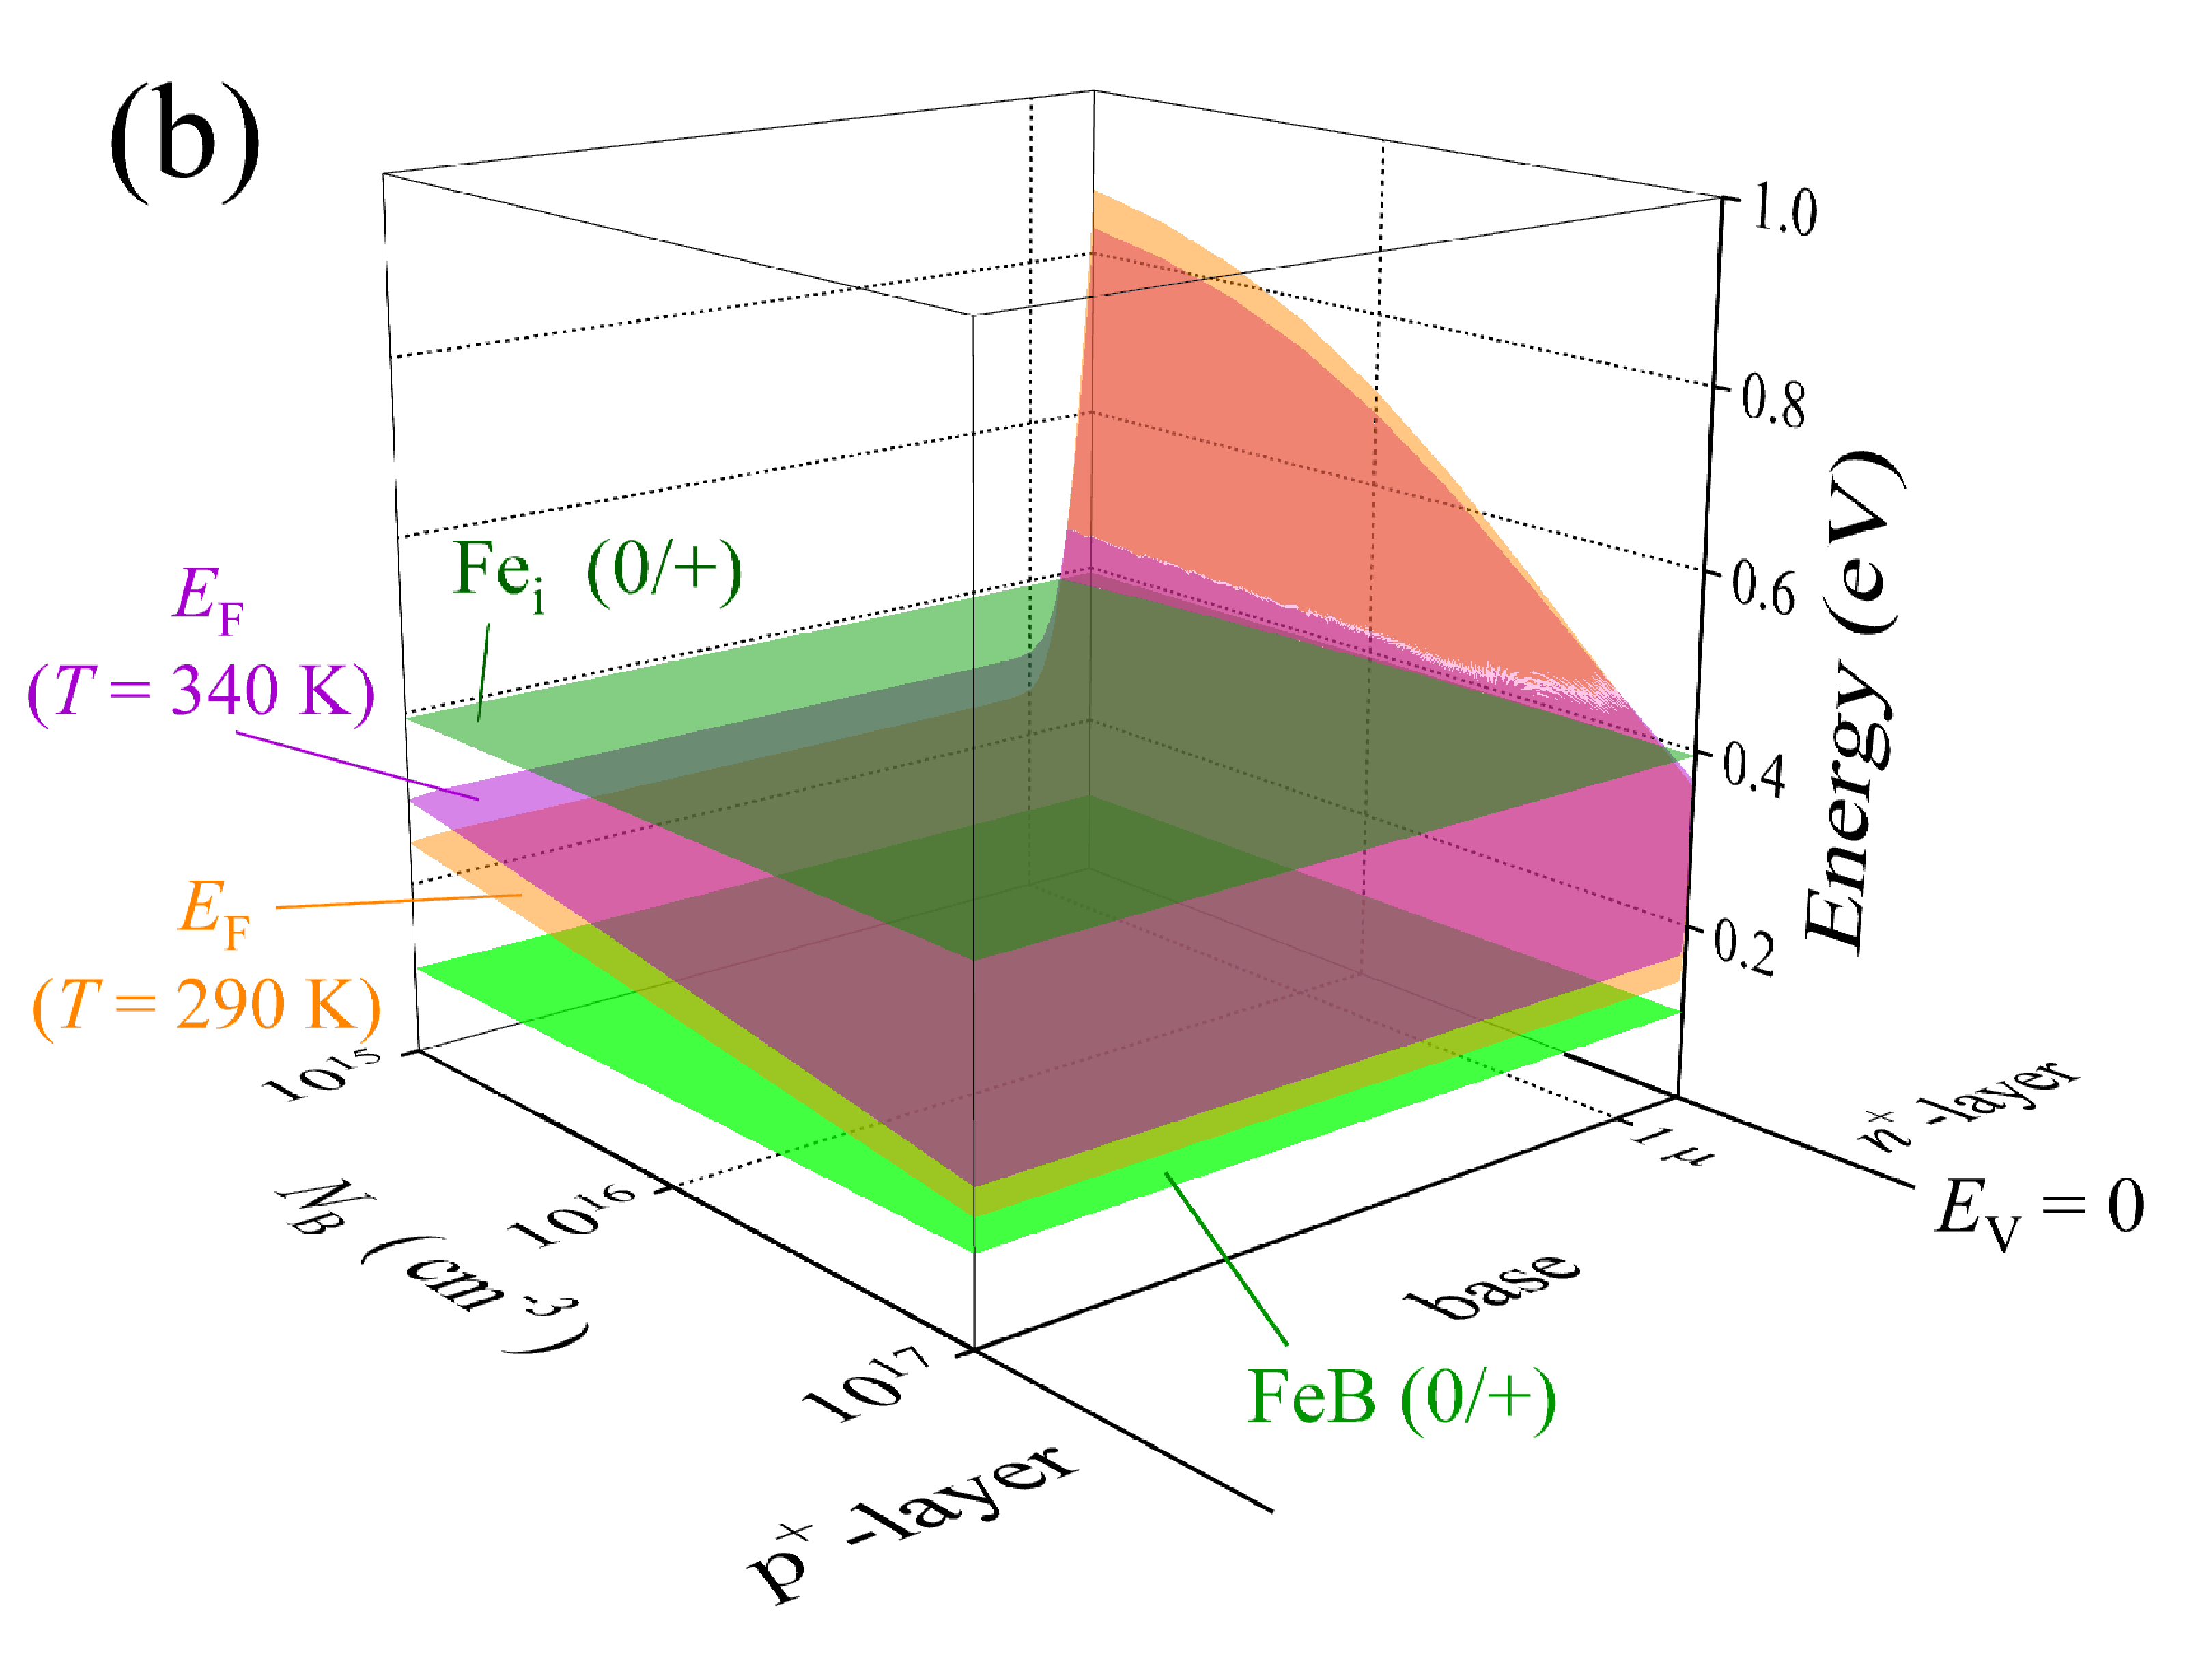
\includegraphics[width=0.49\linewidth]{Fig4b.png}
	  \caption{The location of the Fermi level in the base of the $n^+$-$p$-$p^+$ structure
       as a function of temperature for $N_\mathrm{B}=10^{15}$ and $10^{17}$~cm$^{-3}$ (a),
       and as a function of the doping level for $T=290$ and 340~K (b).
       The zero energy value corresponds to the top of the valence band.
       Also shown are the locations of the donor (0/+) levels for the FeB pair (green surfaces)
       and the interstitial iron atom Fe$_i$ (olive surfaces) and acceptor (-/0) level for FeB pair (brown surfaces).
}\label{fig4}
\end{figure}

In our opinion, the change in sign and the monotonic decrease of $\varepsilon I_\mathrm{SC}$
with increase in doping level value
reflect the change in recombination activity caused by the Fermi level shift.
It should be noted that
at low boron concentrations, $E_\mathrm{F}$ in all points of the base is located below the donor level of Fe$_i$,
while at $N_\mathrm{B}>10^{16}$~cm$^{-3}$,
they intersect in the vicinity of the $p$–$n$ junction --- see Fig.~\ref{fig4}.
The weak dependence on base thickness indicates that the second term in parentheses in Eq.~(\ref{eq4}) is significantly smaller than the first.
In addition, when comparing monochromatic and solar illumination,
the latter generates a significantly larger number of non-equilibrium carriers in the emitter
due to shorter-wavelength photons.
As a result, the emitter current under AM1.5 illumination increases,
which, as shown in Eq.~(\ref{eq3}), leads to a decrease in $\varepsilon I_\mathrm{SC}$ value.

Fig.~\ref{fig5} illustrates the alterations in the short-circuit current,
both observed in experimental studies and calculated for structures with identical base parameters.
It should be noted that the figure shows simulation results obtained at various levels of illumination,
confirming that $\varepsilon I_\mathrm{SC}$ is independent of $W_\mathrm{ill}$.


\begin{figure}
	\centering
     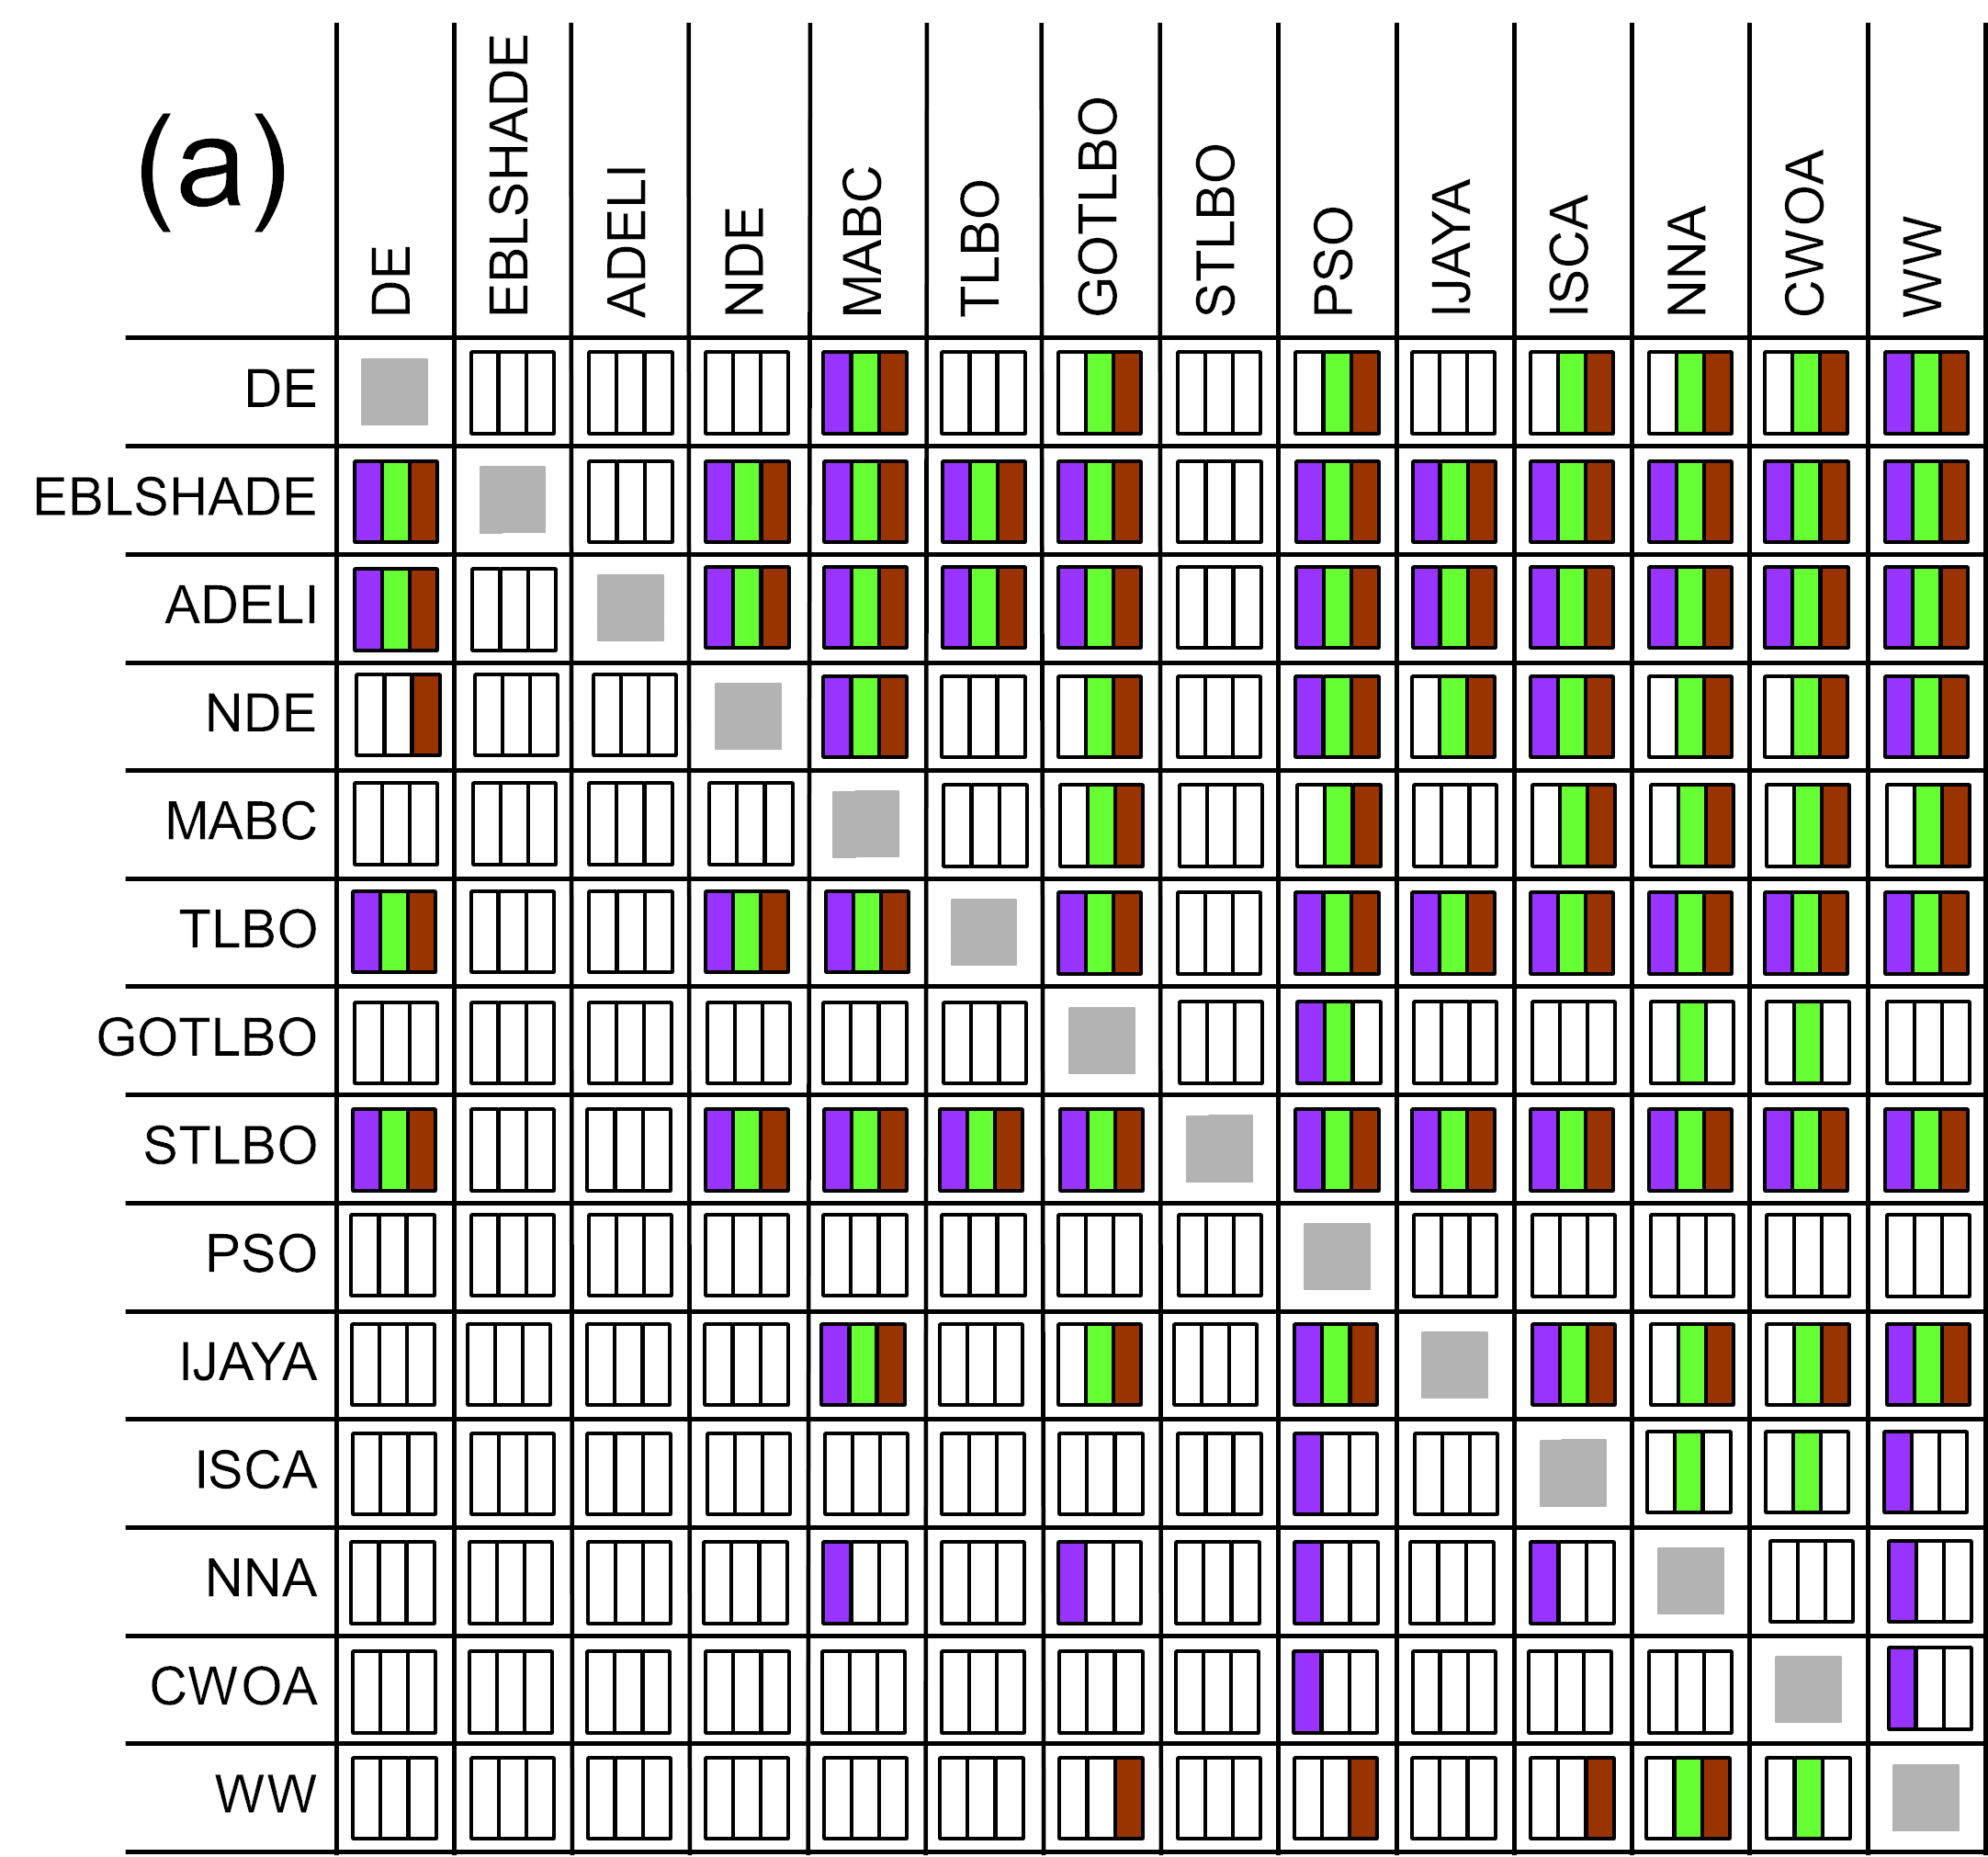
\includegraphics[width=0.4\linewidth]{Fig5a.png}
     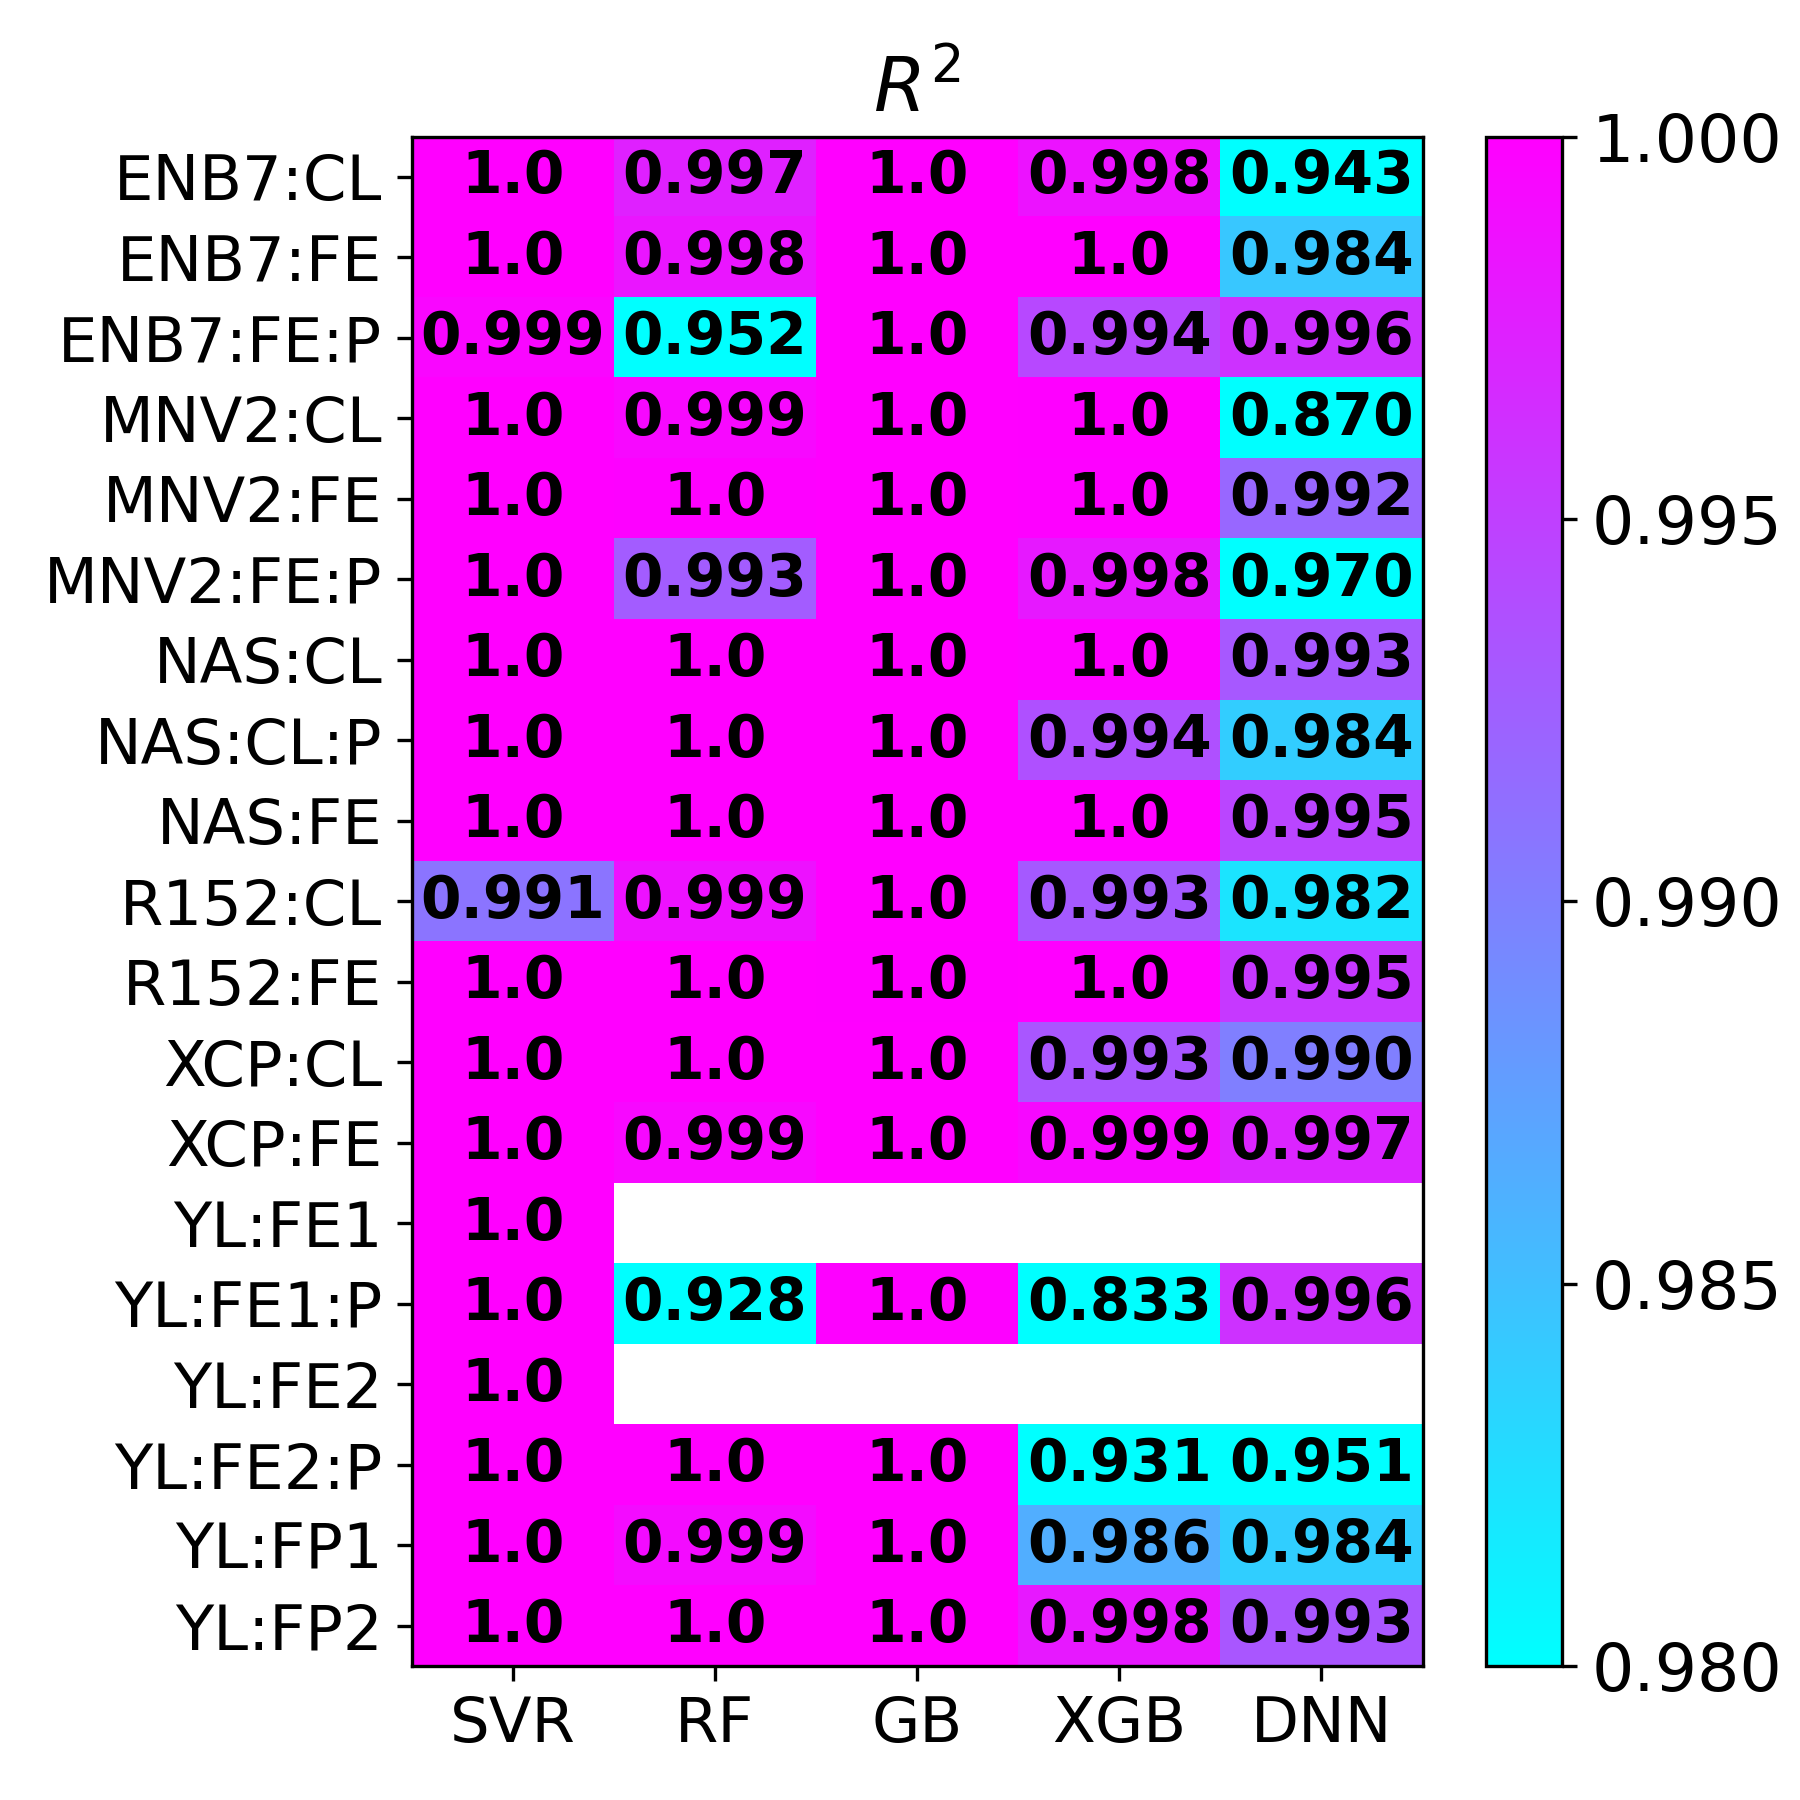
\includegraphics[width=0.4\linewidth]{Fig5b.png}
	  \caption{Relative changes in short-circuit current caused by a complete
       dissociation of Fe$_i$B$_s$ pairs as a function of iron concentration (a) and
       temperature (b) for SSC with $d_p=380$~$\mu$m and $N_\mathrm{B}=1.36\times10^{15}$~cm$^{-3}$
       in the case of monochromatic (940~nm) illumination.
       The marks are the experimental results (divided by factor $C_{cor}=1.4$), the lines are the simulation results.
       $W_\mathrm{ill}$, Wm$^{-2}$: 5 (marks and solid lines), 10 (dotted lines).
       Different lines and marks correspond to different temperatures (a) or $N_\mathrm{Fe}$ values (b) --- see legends.
}\label{fig5}
\end{figure}

One can see that the theoretical dependencies of $\varepsilon I_\mathrm{SC}$
on iron concentration and temperature qualitatively agree with the experimental results.
To achieve quantitative agreement, a correction factor of $C_\mathrm{cor} = 1.4$ must be applied:
the experimentally obtained value $I_\mathrm{SC,exp}$ should be replaced by $I_\mathrm{SC,exp} / C_\mathrm{cor}$ --- as illustrated in Fig.~\ref{fig5}.
This methodology is frequently cited in the literature \cite{IronSC} and is associated with correcting specific systematic errors in simulations.
In our case, these errors may arise because certain factors present in actual SSCs were not accounted for in the calculations, specifically:

\noindent
- the possible influence of series and shunt resistances;

\noindent
- the antireflective SiO$_2$ and passivating Si$_3$N$_4$ layers on the front surface induce a spectral dependence in reflectance, corresponding calculations necessitating the consideration of multiple reflections \cite{KostRefl2000};

\noindent
- the shading caused by electrodes;

\noindent
- the presence of defects unrelated to iron.


Given the study's primary objective,
the relative changes in short-circuit current after the complete dissociation of FeB pairs
can be used to estimate iron concentration:
$\varepsilon I_\mathrm{SC}$ depends monotonically on $N_\mathrm{Fe}$, and its values can be pretty significant.
In this context, determining the amount of impurity atoms is more appropriately conducted
using photovoltaic parameters obtained under monochromatic illumination,
as this method offers greater sensitivity (response amplitude of $\varepsilon I_\mathrm{SC}$).
However, it should be noted that for low iron concentrations ($N_\mathrm{Fe}<10^{11}$~cm$^{-3}$)
and solar cells with boron concentrations in the base around $10^{16}$~cm$^{-3}$,
this approach appears to be unproductive.
At these levels, there are blind spots in determining impurity metal concentrations.


\subsection{Open-circuit voltage}

Figure~\ref{fig7} presents the characteristic simulation results of open-circuit voltage changes due to the dissociation of FeB pairs.
Figures~S7--S12 in the Supplementary Material show additional $\varepsilon V_\mathrm{OC}$ dependencies.
Notably, the changes in $V_\mathrm{OC}$ value are almost an order of magnitude smaller than the values observed for $I_\mathrm{SC}$.
Moreover, differences in the behavior of open-circuit voltage changes as a function of iron concentration
at low ($N_\mathrm{B}<2\times10^{16}$~cm$^{-3}$) base doping levels
in the cases of monochromatic and AM1.5 illumination are noteworthy.
Under solar illumination, $\varepsilon V_\mathrm{OC}$ values are negative,
and the $\varepsilon V_\mathrm{OC} \left(N_\mathrm{Fe}\right)$ dependency is non-monotonic --- see figs.~\ref{fig6}a,~\ref{fig6}b.
Additionally, the base thickness significantly impacts the iron concentration,
which correlates with the minimum $\varepsilon V_\mathrm{OC}$ value (Fig.~\ref{fig6}a).
When illuminated by photons with a wavelength of 940~nm, $\varepsilon V_\mathrm{OC}$ values are positive and increase monotonically with iron concentration.
As boron concentration increases, the behavior of $\varepsilon V_\mathrm{OC}\left(N_\mathrm{Fe}\right)$ becomes similar, regardless of the type of illumination:
the relative changes in open-circuit voltage during the rebuilding of iron-containing defects
are negative and increase monotonically in absolute value with increasing both $N_\mathrm{Fe}$ and $N_\mathrm{B}$.
Furthermore, changes in $V_\mathrm{OC}$ are more significant under monochromatic illumination, similar to the case of the short-circuit current.


\begin{figure}
	\centering
     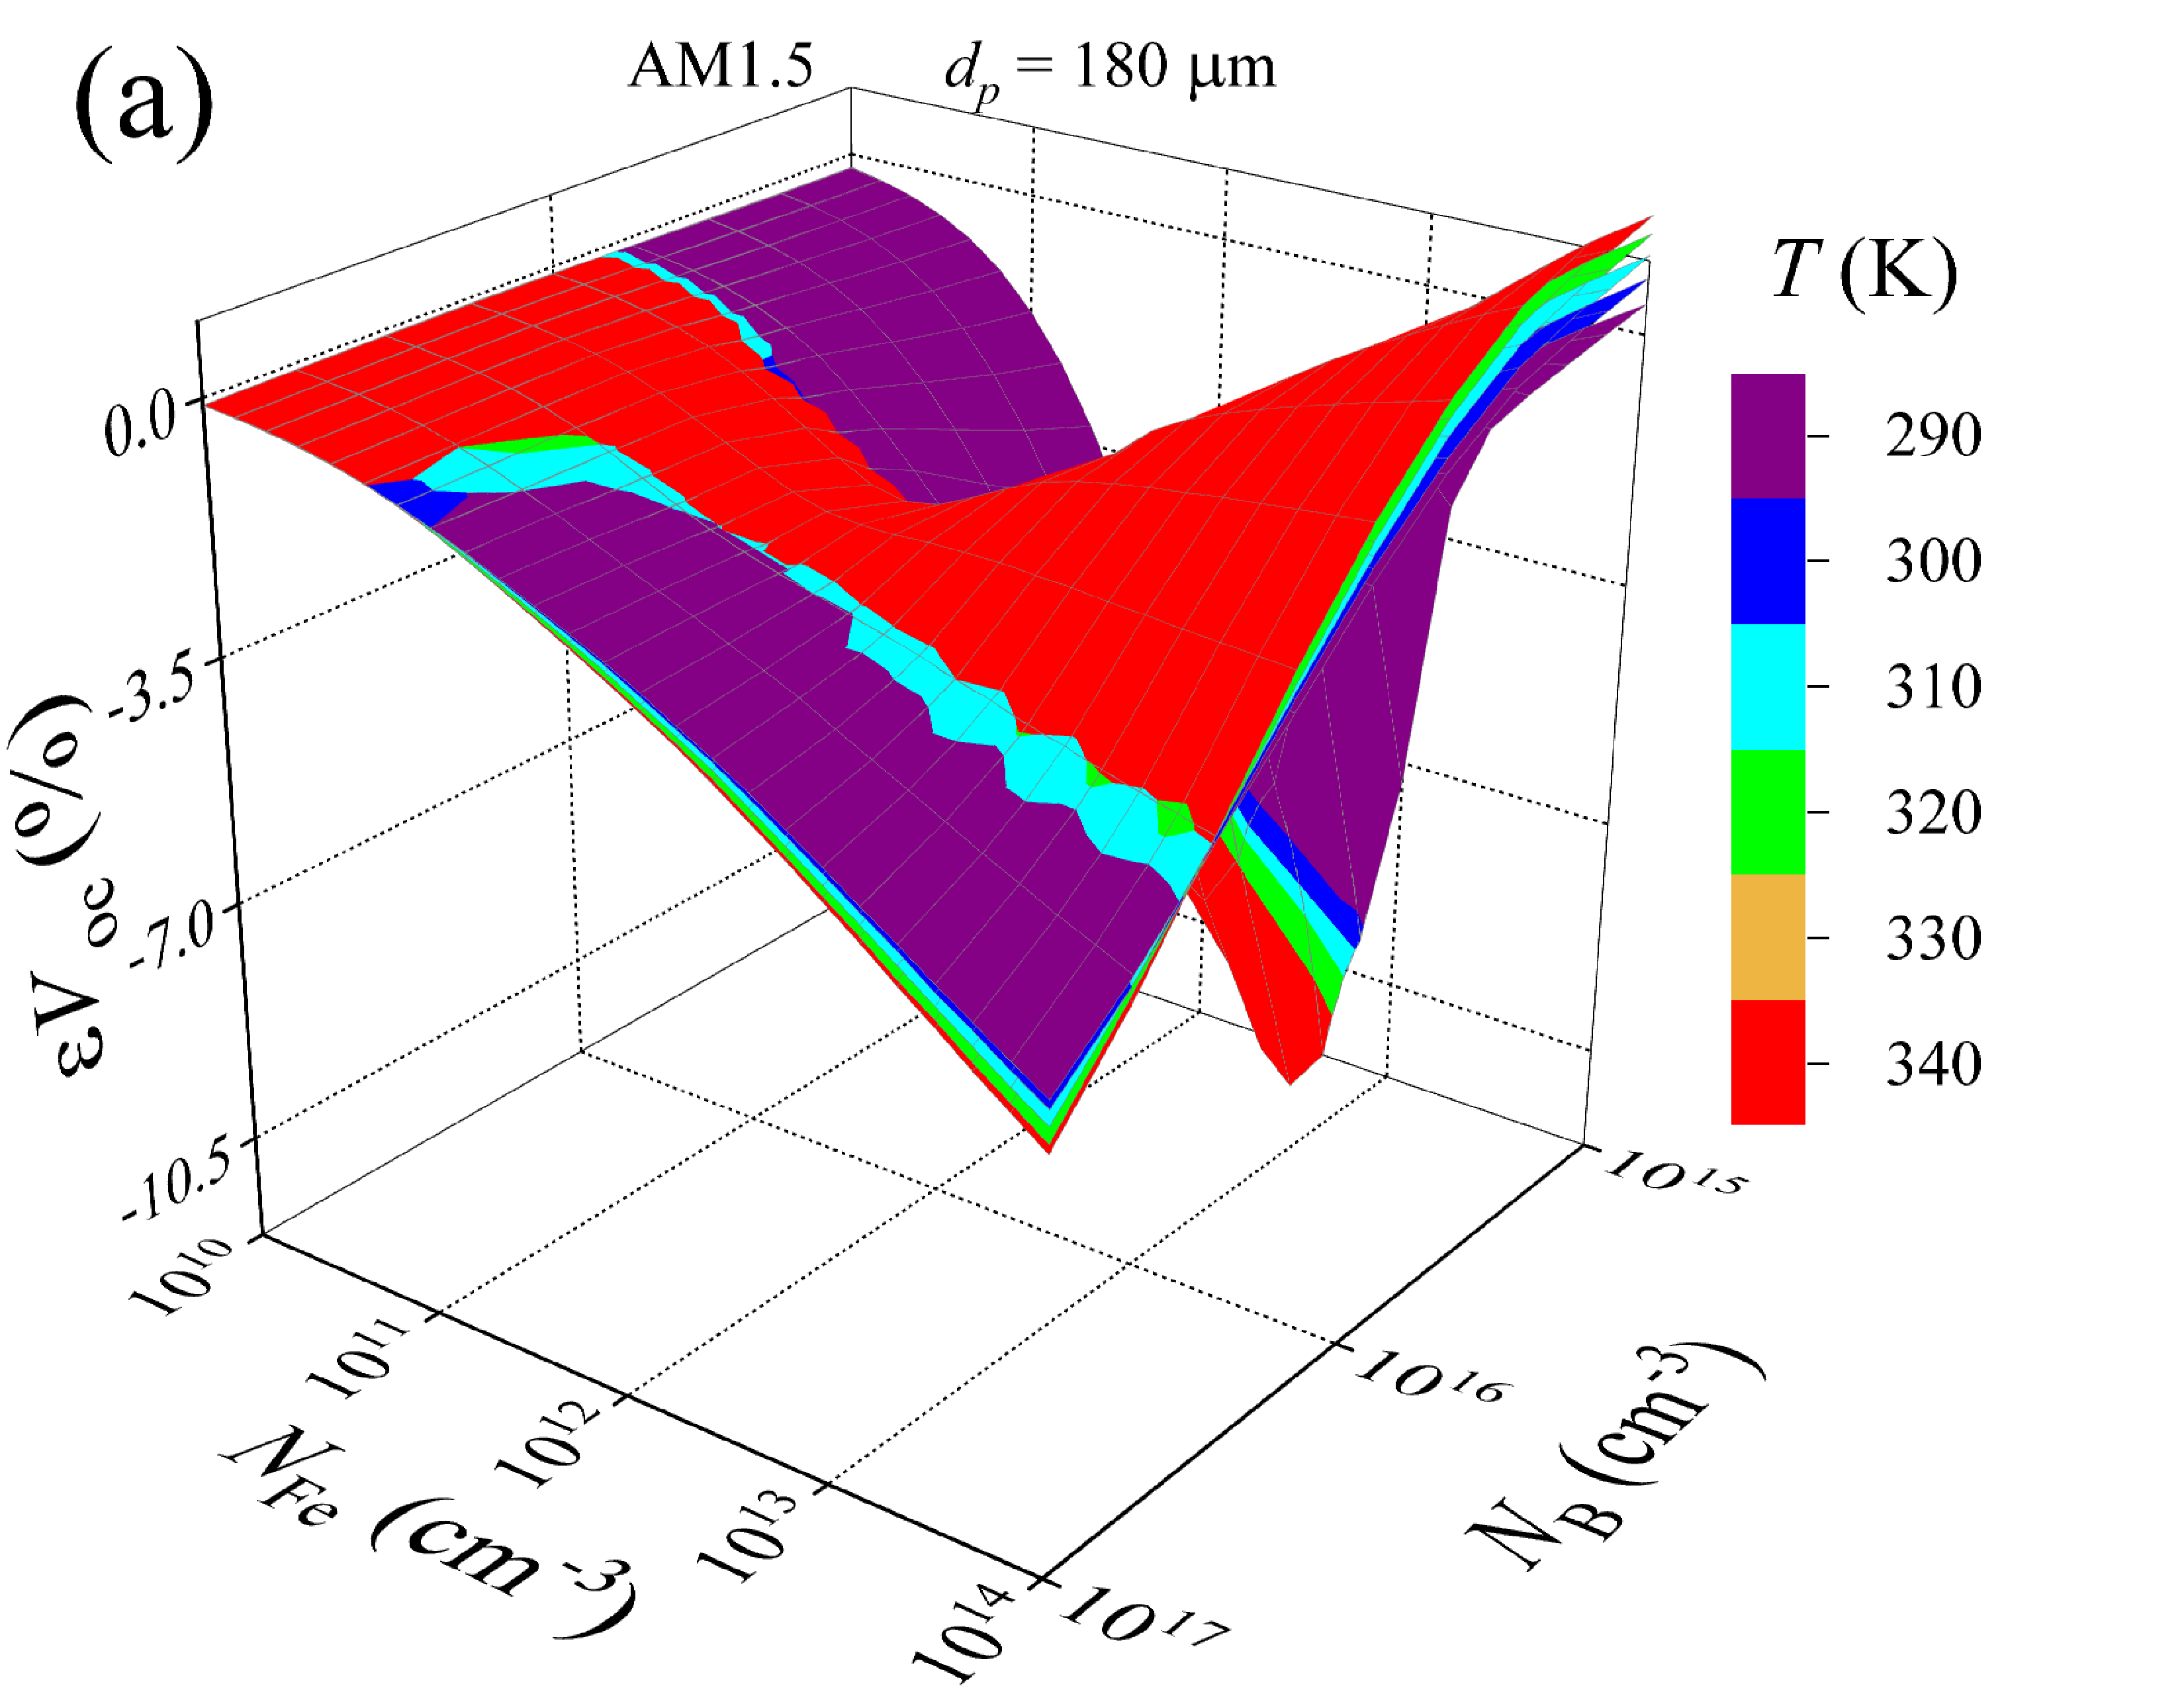
\includegraphics[width=0.49\linewidth]{Fig6a.png}
     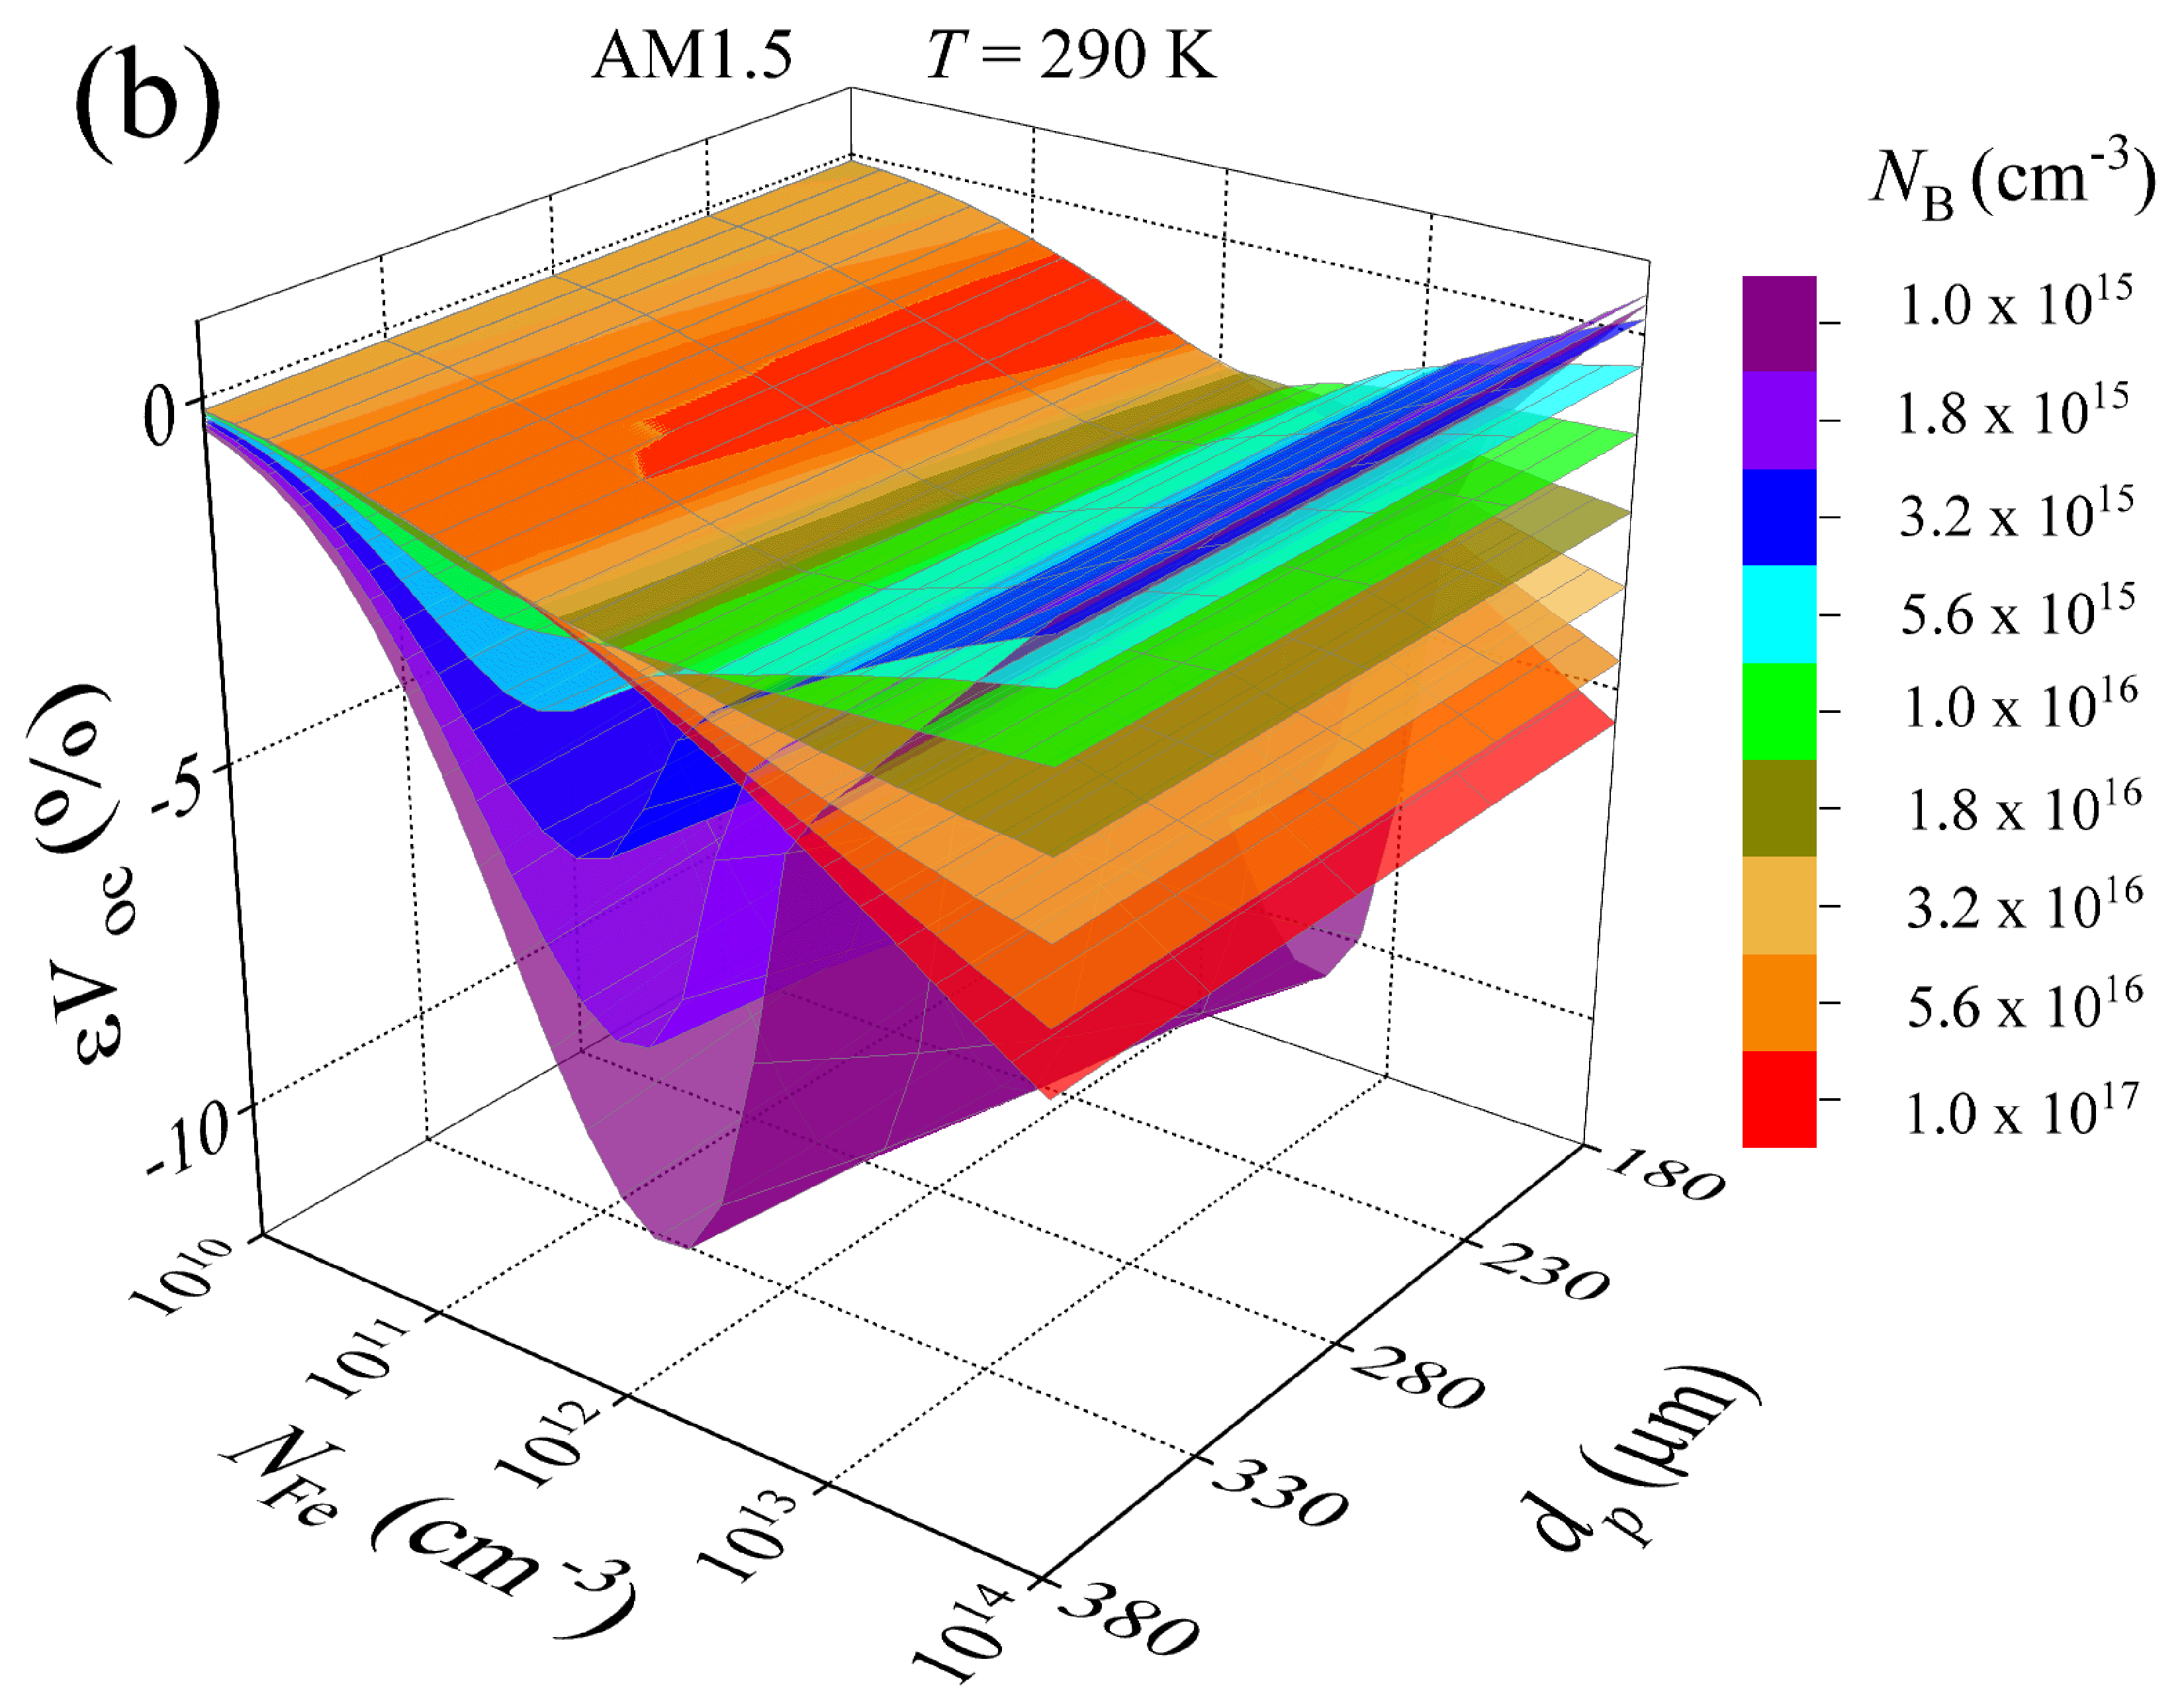
\includegraphics[width=0.49\linewidth]{Fig6b.png}
     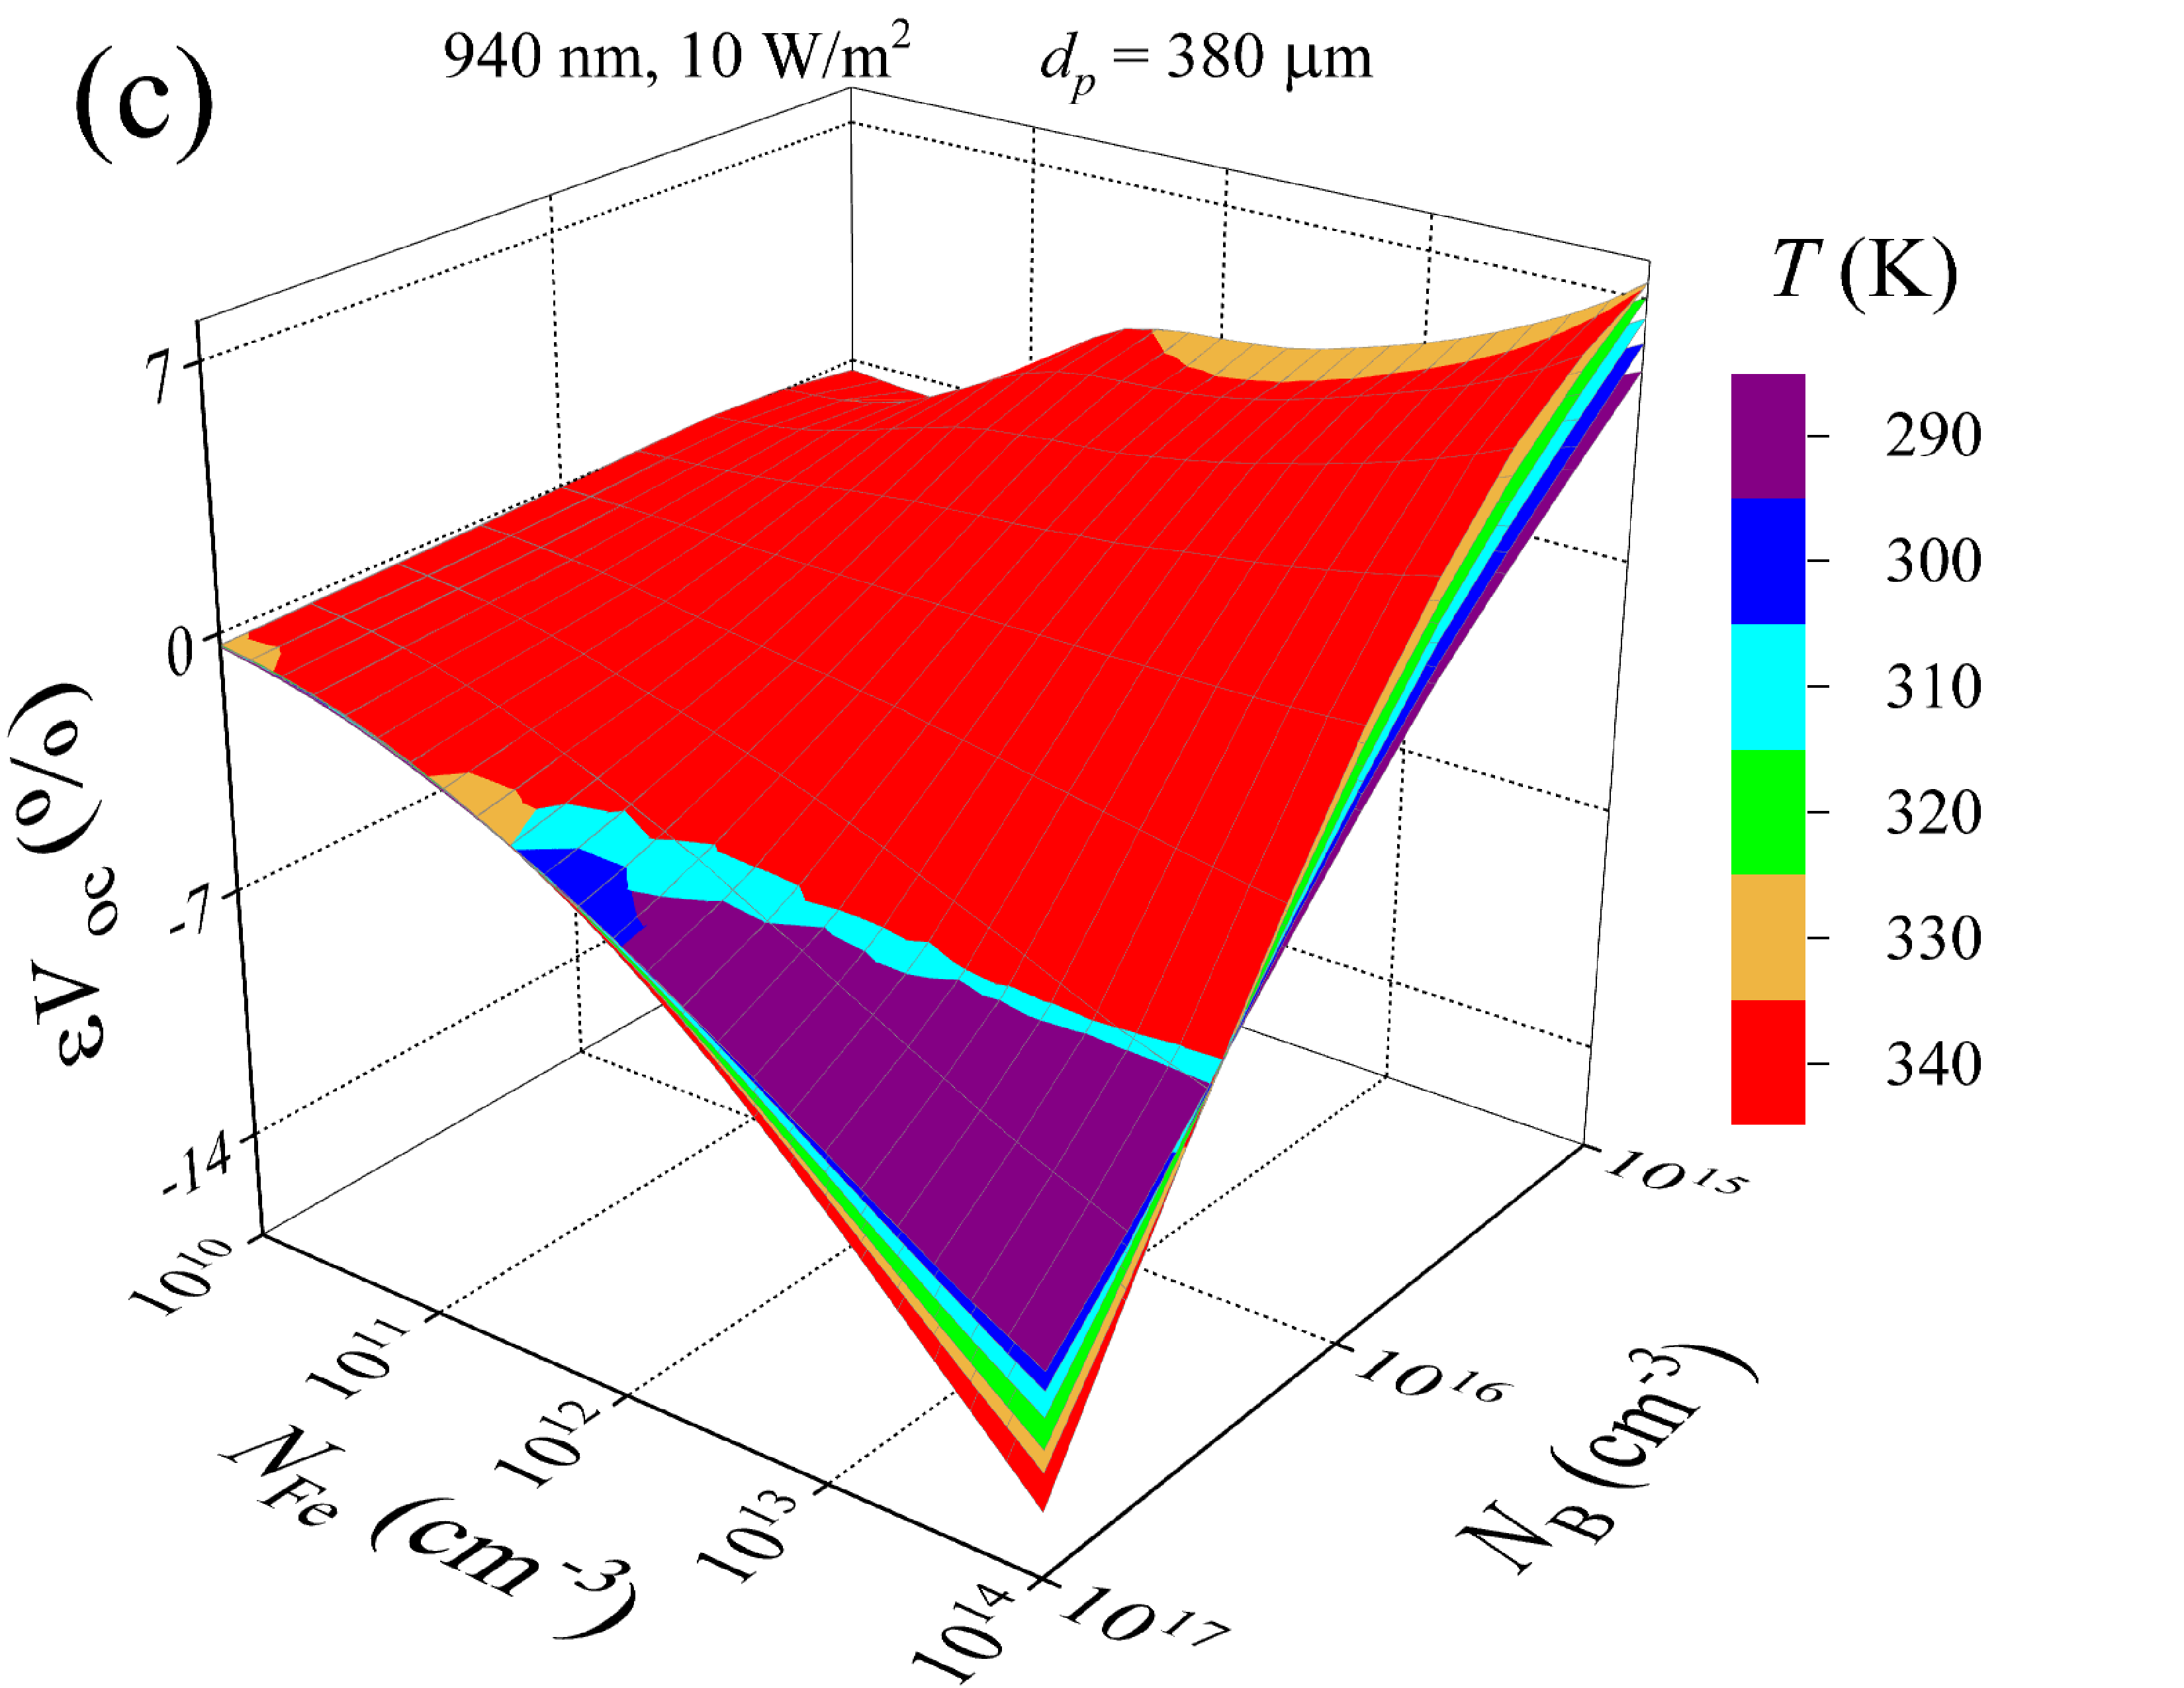
\includegraphics[width=0.49\linewidth]{Fig6c.png}
     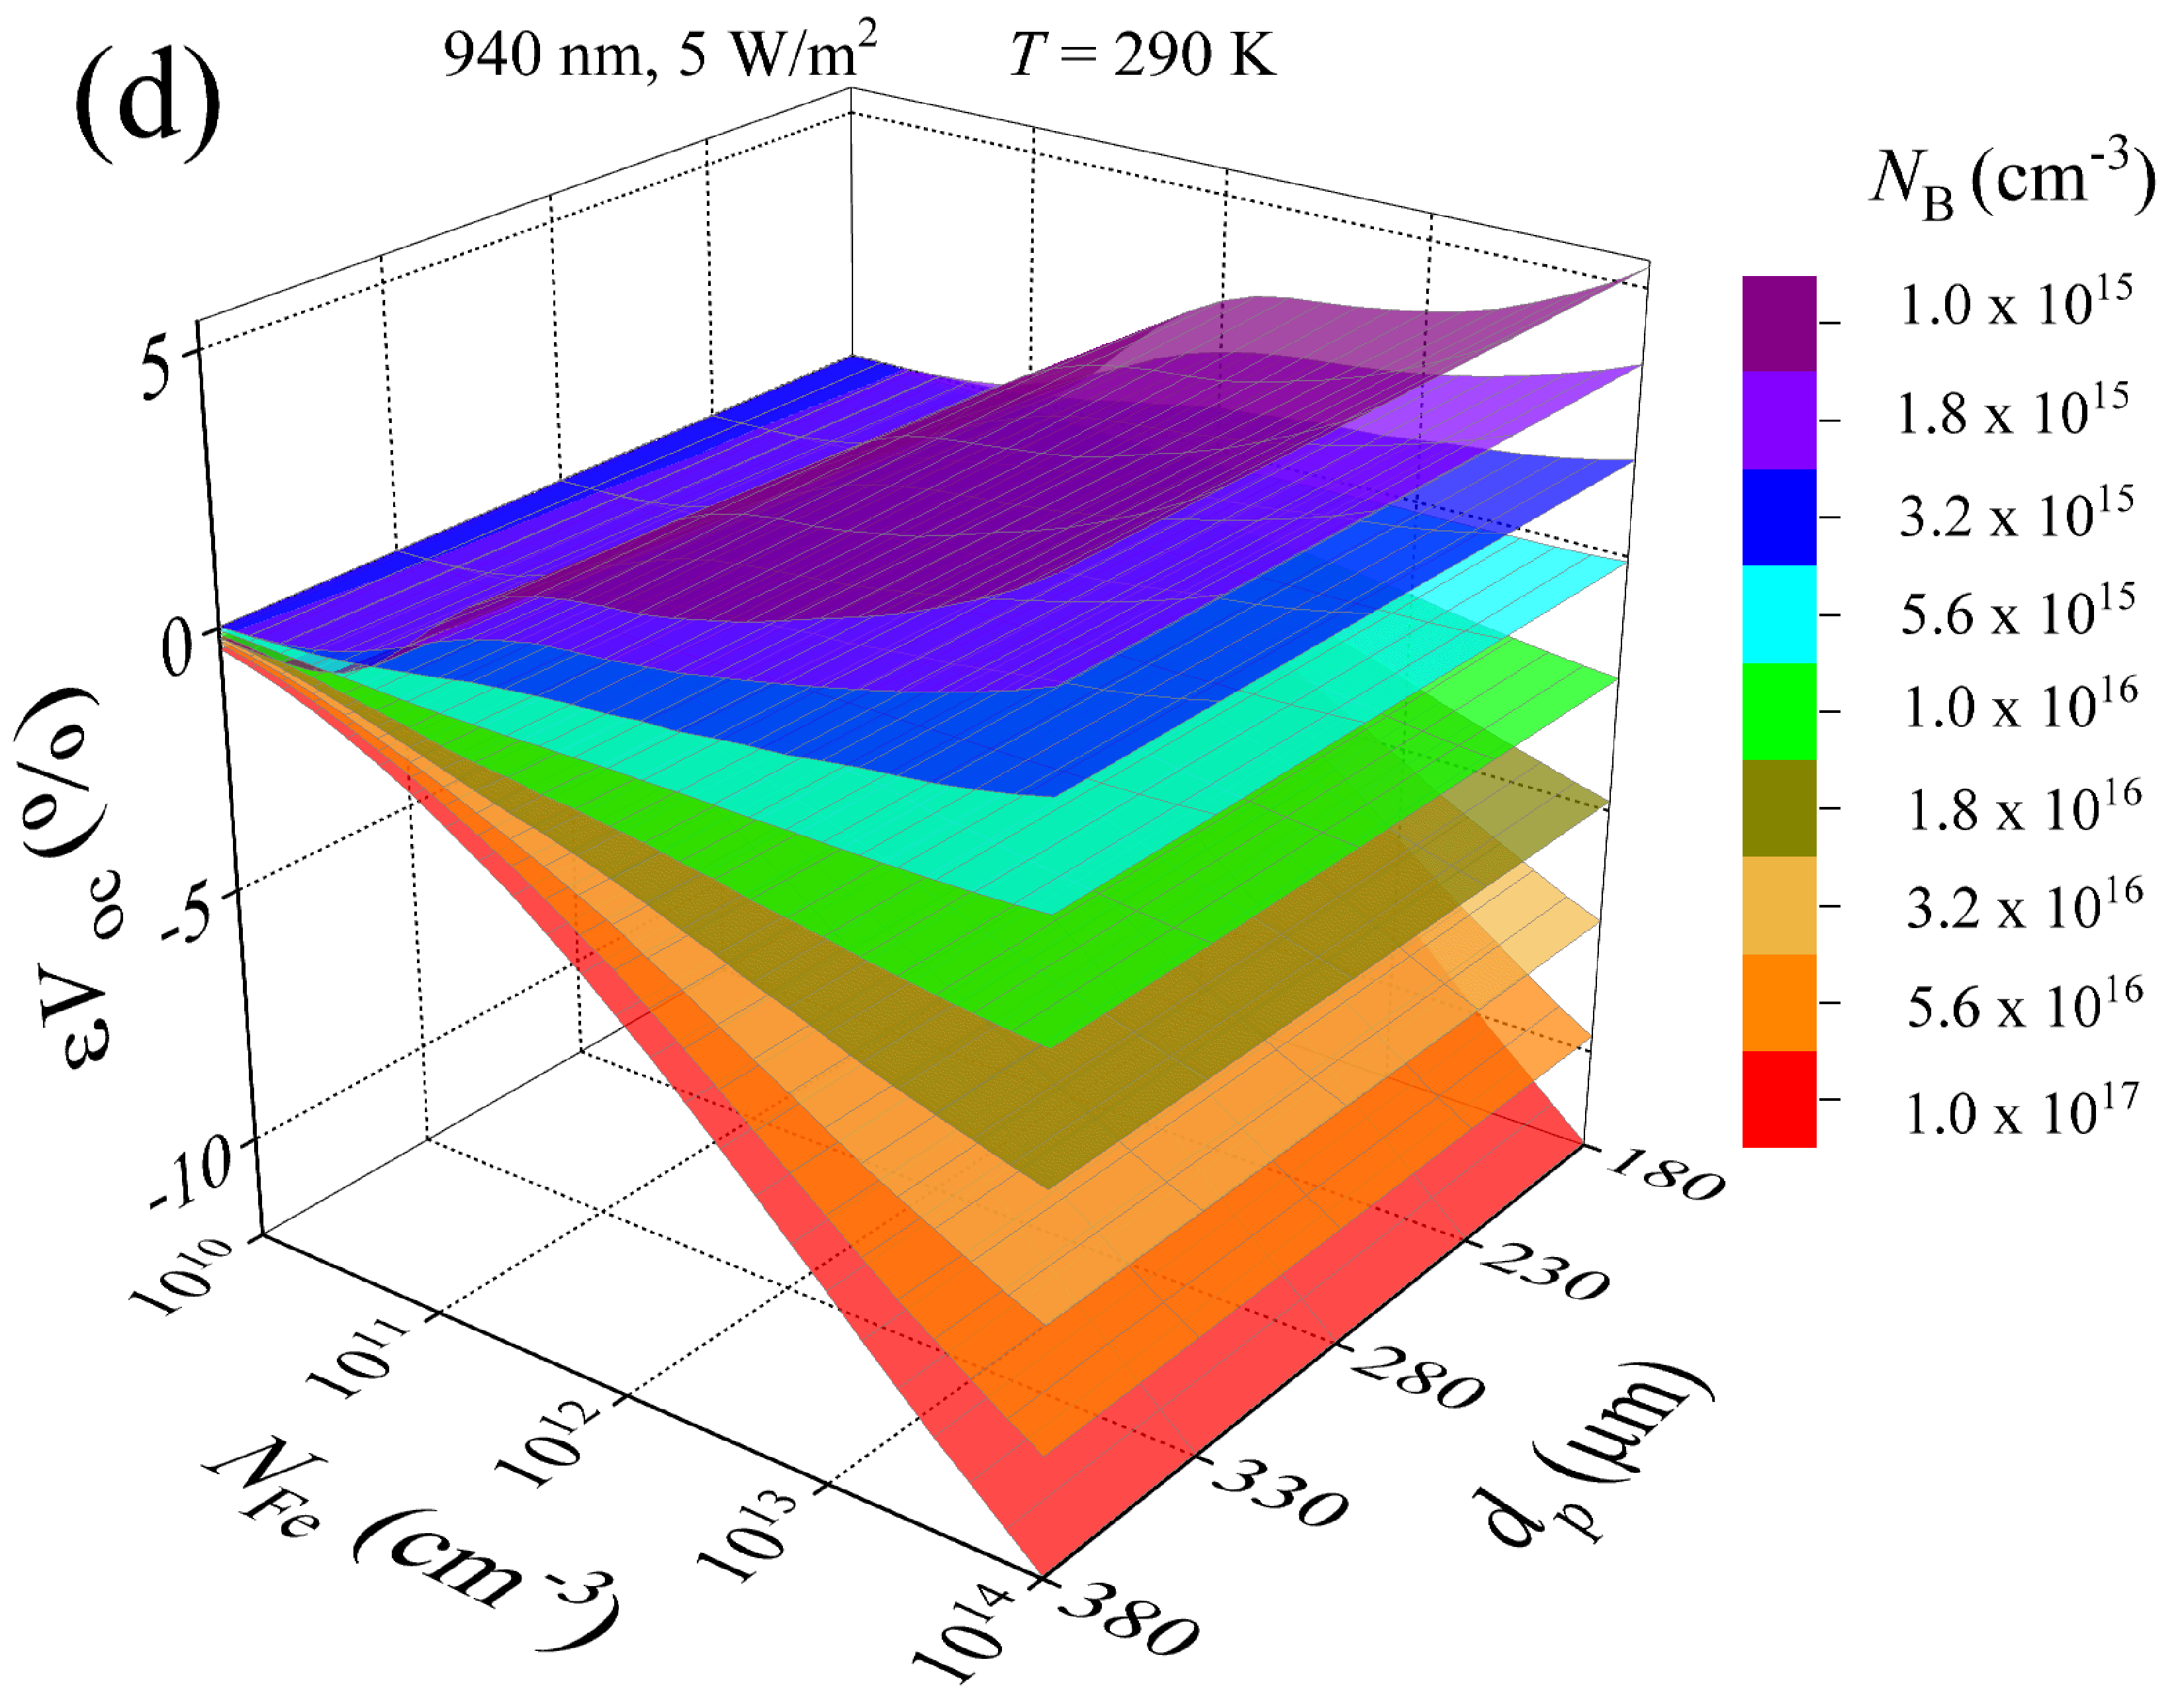
\includegraphics[width=0.49\linewidth]{Fig6d.png}
	  \caption{Relative changes in open-circuit voltage caused by a complete
       dissociation of Fe$_i$B$_s$ pairs as a function of
       iron concentration and
       doping level (panels a and c) or base depth (b, d).
       Illumination: AM1.5 (a, b), 940~nm 10~Wm$^{-2}$ (c),  940~nm 5~Wm$^{-2}$ (d).
       $T$, K: 290 (b, d).
       Different surfaces correspond to different temperatures (a, c) and doping levels (b, d).
}\label{fig6}
\end{figure}

The effect of temperature on $\varepsilon V_\mathrm{OC}$ also depends on the base doping level:
as $N_\mathrm{B}$ increases, the temperature coefficient of $\varepsilon V_\mathrm{OC}$ gradually shifts from positive to negative.
This trend is observed for both AM1.5 and 940nm illumination, as shown in Figs.~S9,~\ref{fig6}a, and \ref{fig6}b.
The impact of $d_p$ on changes in open-circuit voltage is more significant than the effect observed for $\varepsilon I_\mathrm{SC}$.
However, base thickness is not a determining factor for $\varepsilon V_\mathrm{OC}$;
it mainly affects low doping levels and temperatures, as shown in Figs.~S9, S11, and S12.
Another difference between the behavior of $\varepsilon V_\mathrm{OC}$ and $\varepsilon I_\mathrm{SC}$
is the former dependence on monochromatic illumination intensity.
At $W_\mathrm{ill} = 10$~Wm$^{-2}$, changes in open-circuit voltage are less significant,
with differences increasing as iron concentration decreases and showing weak temperature dependence.

Understanding the features of $\varepsilon V_\mathrm{OC}$ requires recalling
that the open-circuit voltage depends not only on the photocurrent
but also on the saturation current $I_0$ and the ideality factor,
which in turn are determined by the state of the defect subsystem and other parameters
that varied in simulation \cite{Olikh2019SM,YangHandbookPVSi}.
In the case of simplified single-diode model \cite{YangHandbookPVSi}:
\begin{equation}
\label{eq5}
     V_\mathrm{OC} = nkT\left[ {\ln\left( {\frac{I_\mathrm{ph}}{I_0}} \right)+1} \right]\,.
\end{equation}

Similar to the photocurrent, we can express $I_\mathrm{0}$ as the sum of the currents from the base and the emitter \cite{Markvart}:
\begin{equation}
\label{eq6}
     I_0 = I_\mathrm{0,e}+I_\mathrm{0,b}\,,
\end{equation}
and the second term can be expressed as follows \cite{Goetzberger1998}:
\begin{equation}
\label{eq7}
     I_\mathrm{0,b}=\frac{qn_i D_n}{N_\mathrm{B}L_n}\cdot\frac{\frac{D_n}{SL_n}\sinh\left( \frac{d_p}{L_n} \right)+\cosh\left( \frac{d_p}{L_n} \right)}{\sinh\left( \frac{d_p}{L_n} \right)+\frac{D_n}{SL_n}\cosh\left( \frac{d_p}{L_n} \right)}\,,
\end{equation}
where
$n_i$ is the intrinsic carrier concentration.
The last equation explains the observed dependence of $\varepsilon V_\mathrm{OC}$ on the base thickness.

It was shown \cite{Olikh2022PPV,Olikh2019SM} previously
that changes in the ideality factor during restructuring Fe$_i$B$_\mathrm{Si}$ $\rightleftharpoons$ Fe$_i$ + B$_\mathrm{Si}$ do not exceed a few percent.
This $n$ slight variation, combined with the logarithmic dependence of $V_\mathrm{OC}$ on $I_\mathrm{ph}$ as shown in Eq. (\ref{eq5}),
explains the small absolute values of $\varepsilon V_\mathrm{OC}$.

Schmidt \cite{FeB:Schmidt} attributes the non-monotonic dependence of $\varepsilon V_\mathrm{OC}\left(N_\mathrm{Fe}\right)$
(Fig.~\ref{fig6}b) to the significantly higher injection level in the cell base under open-circuit conditions
compared to short-circuit conditions.
Overall, the results support this hypothesis.
In fact,
for monochromatic illumination with significantly lower intensity,
the injection level remains below the crossover point \cite{FeB:Schmidt} throughout the $I$--$V$ curve,
which results in the absence of a minimum in the $\varepsilon V_\mathrm{OC}\left(N_\mathrm{Fe}\right)$ dependence.

The data presented in Fig.~\ref{fig7} compare the experimental and simulation results.
Overall, the results in both cases is qualitatively consistent.
However, to ensure that the absolute values are consistent, a correction factor dependent on iron concentration must be used.
According to the data, $C_\mathrm{cor}$ is less than 1 for low values of $N_\mathrm{Fe}$ and greater than 1 for high values.
By the way, Schubert et al. \cite{IronSC} also observed such dependence of the correction factor.

\begin{figure}
	\centering
     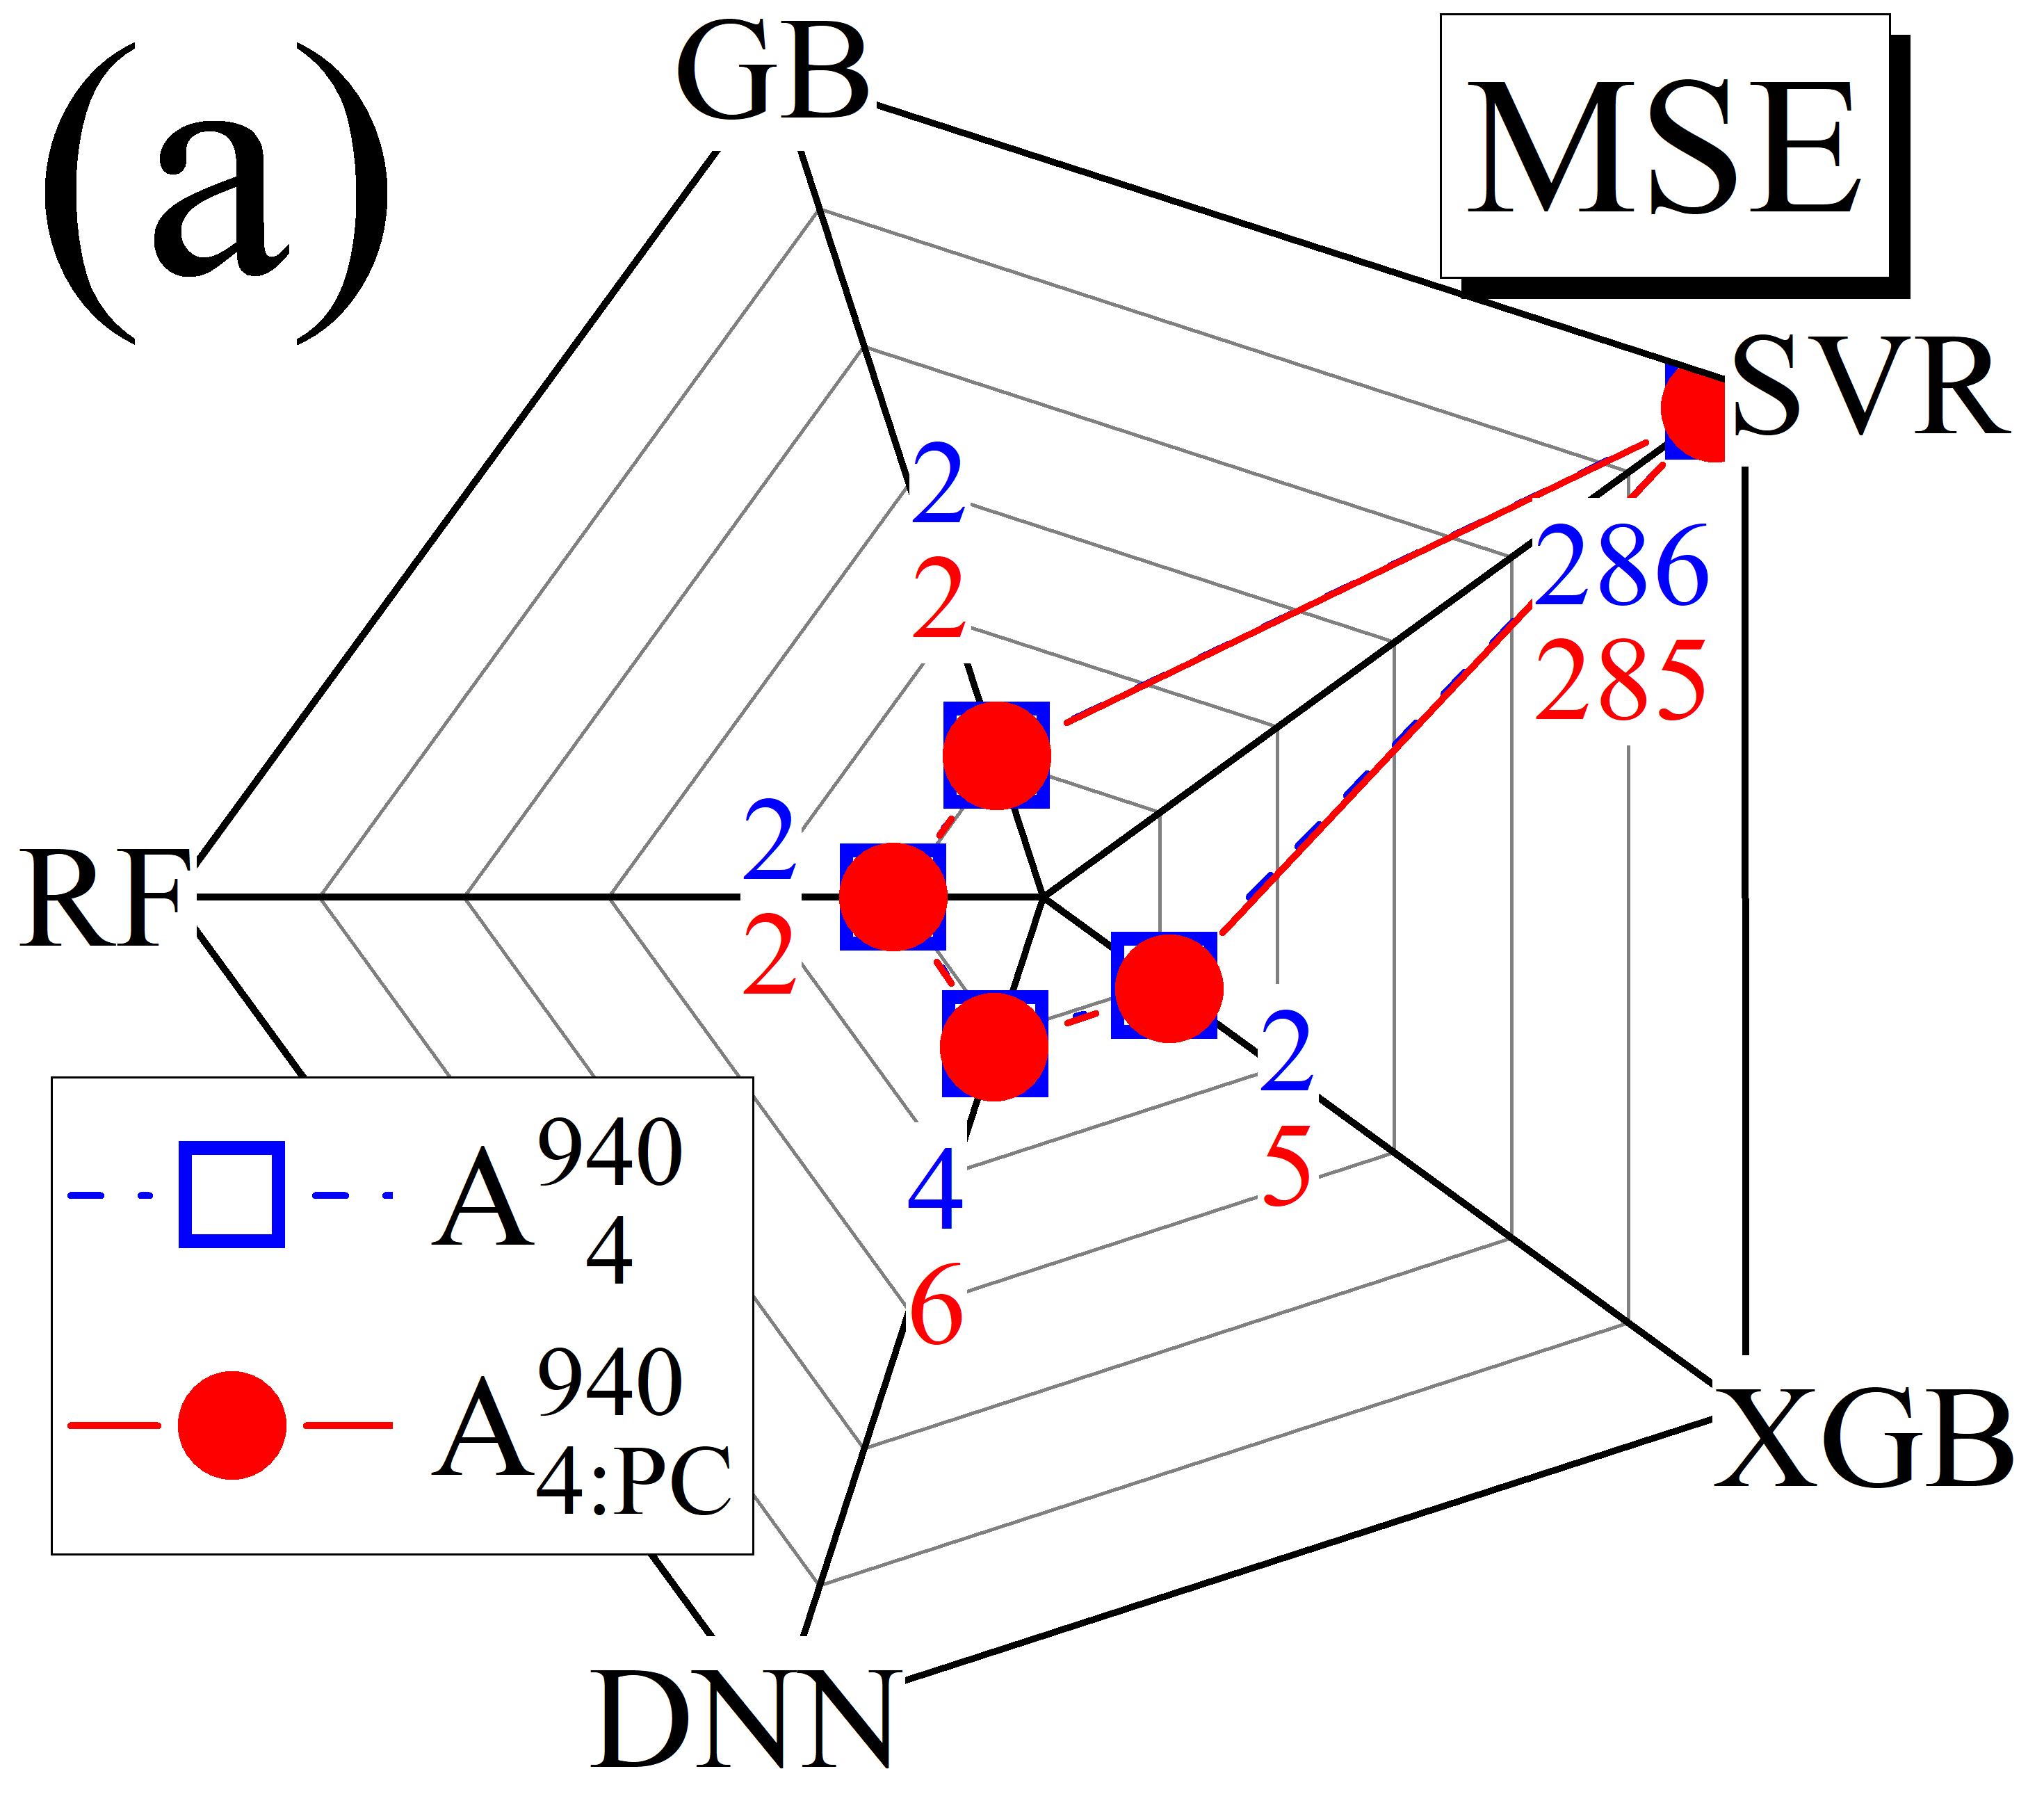
\includegraphics[width=0.4\linewidth]{Fig7a.png}
     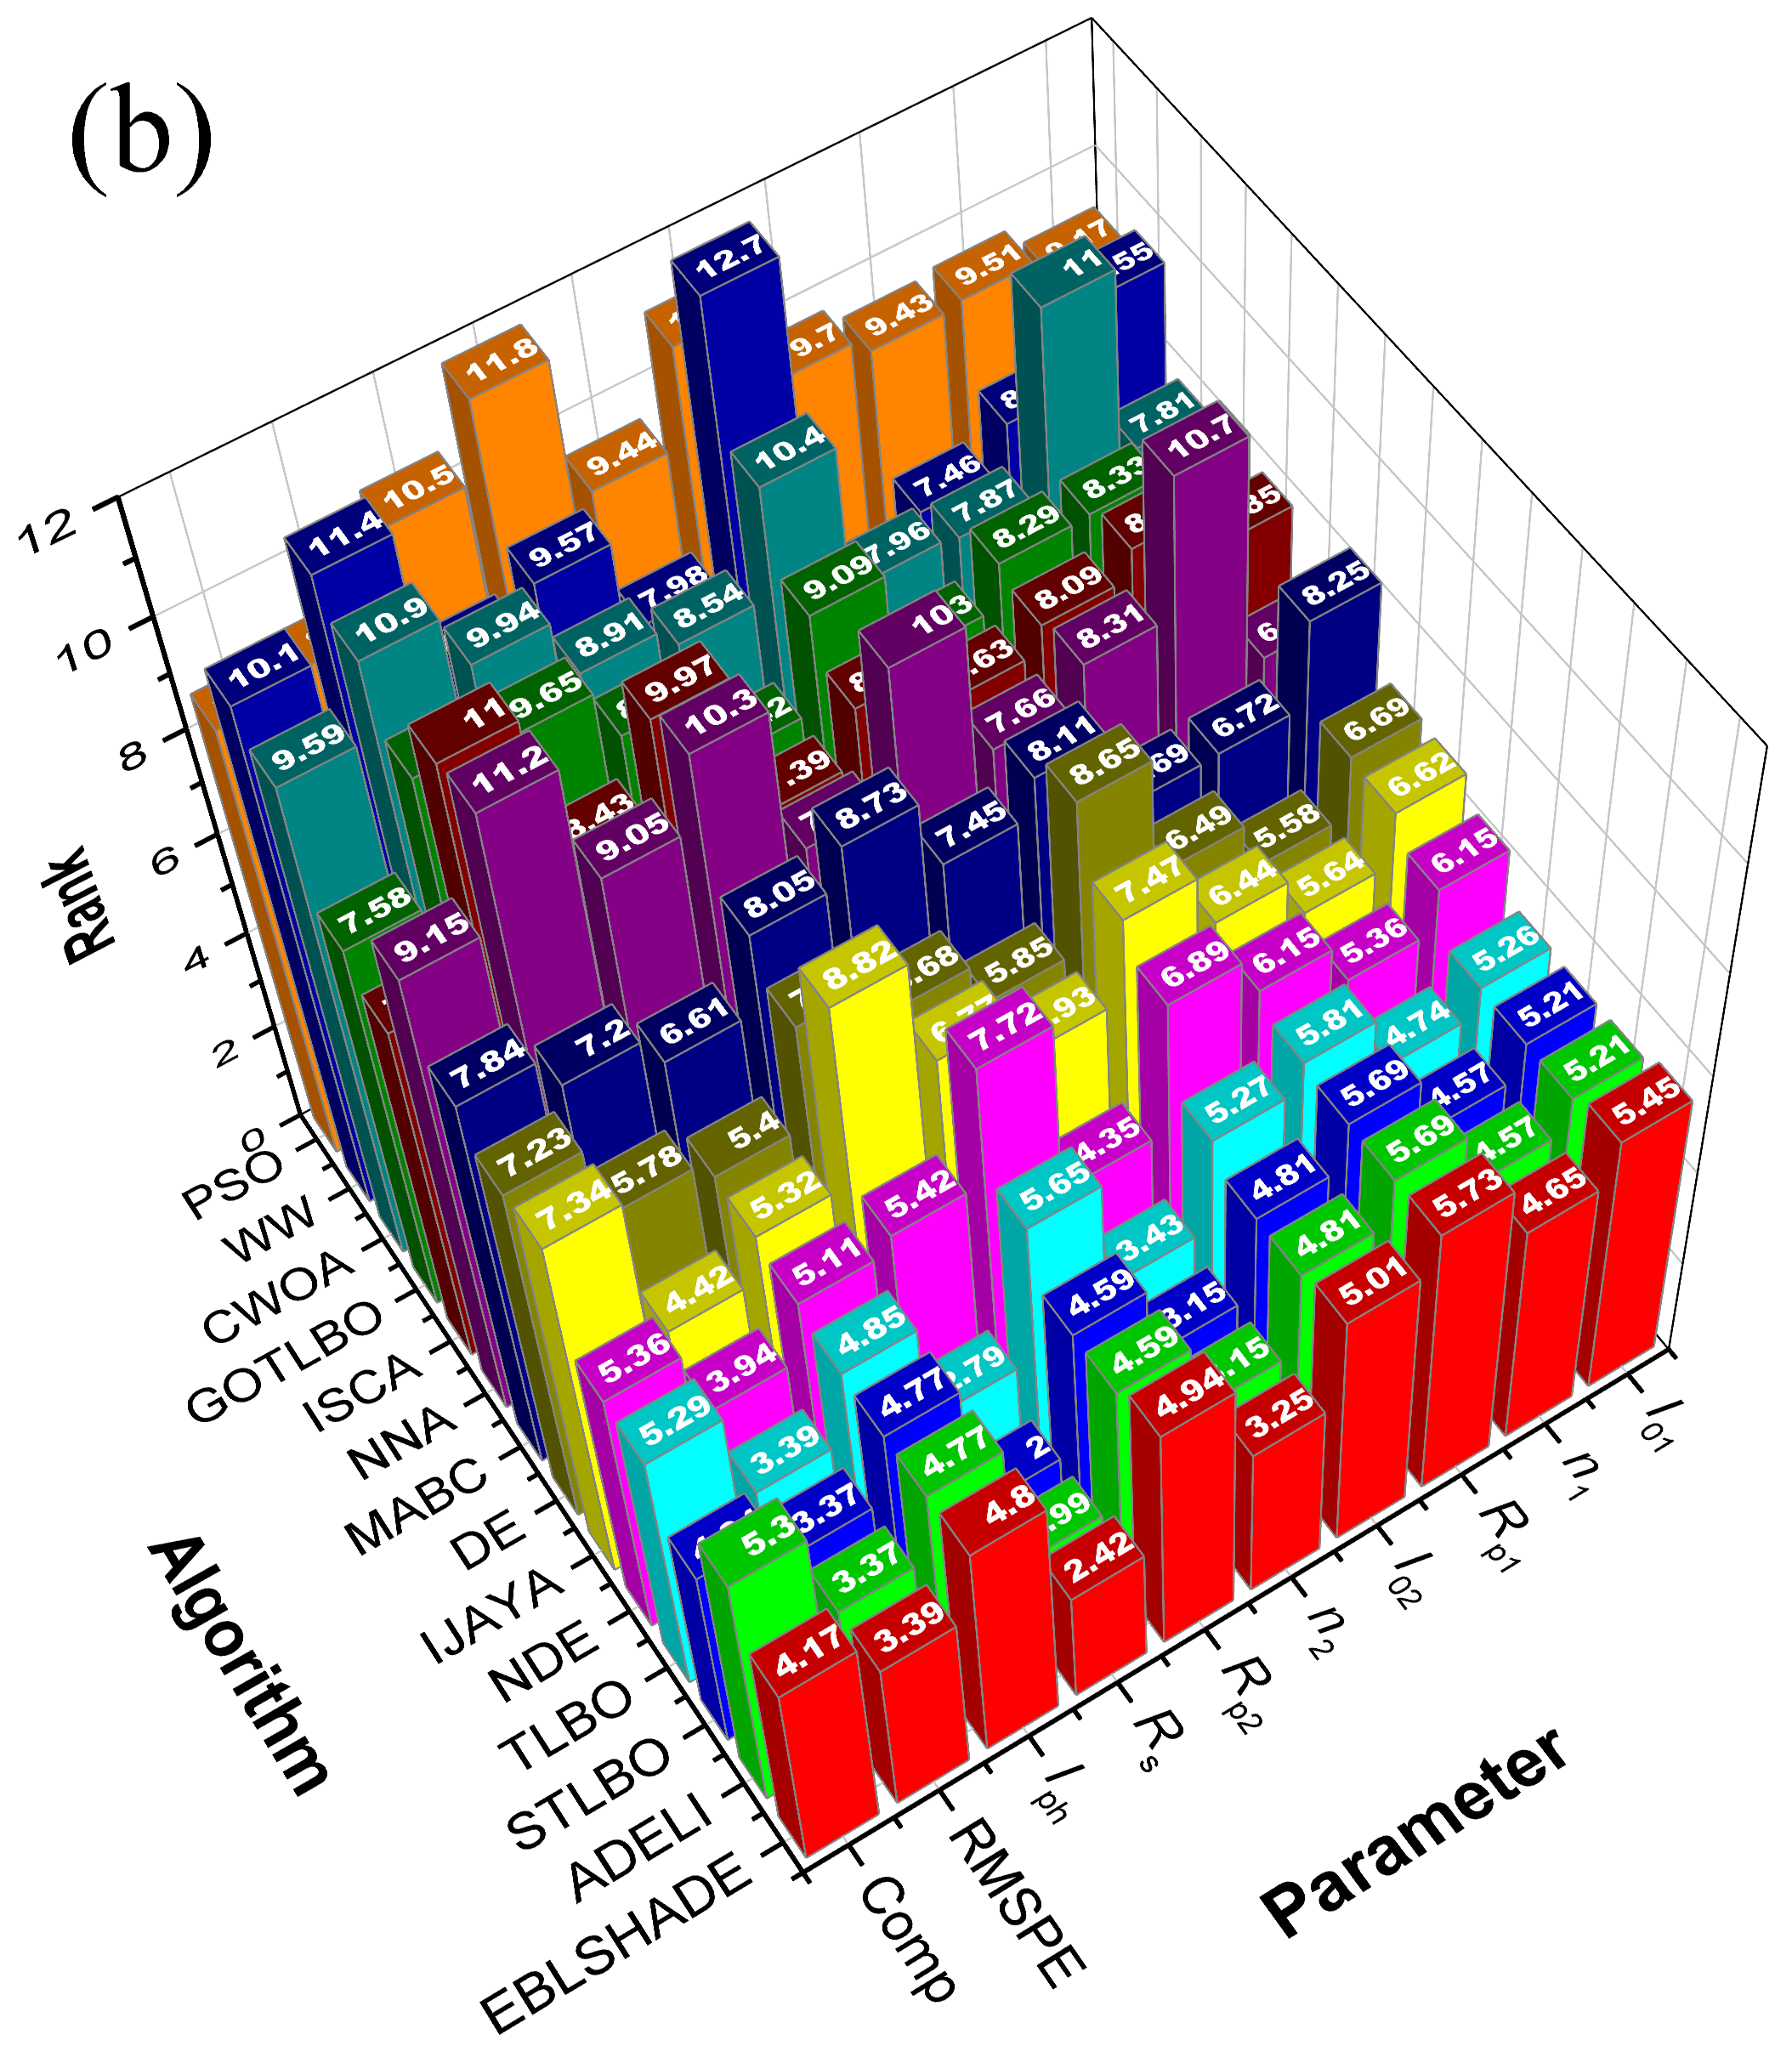
\includegraphics[width=0.4\linewidth]{Fig7b.png}
	  \caption{Relative changes in open-circuit voltage caused by a complete
       dissociation of Fe$_i$B$_s$ pairs as a function of iron concentration (a) and
       temperature (b) for SSC with $d_p=380$~$\mu$m and $N_\mathrm{B}=1.36\times10^{15}$~cm$^{-3}$
       in the case of monochromatic (940~nm) illumination.
       The marks are the experimental results, the lines are the simulation results.
       $W_\mathrm{ill}$, Wm$^{-2}$: 5 (marks and solid lines), 10 (dotted lines).
       Different lines and marks correspond to different temperatures (a) or $N_\mathrm{Fe}$ values (b) --- see legends.
}\label{fig7}
\end{figure}

It is believed \cite{YangHandbookPVSi} that the main effect of metals on the $V_\mathrm{OC}$ values can be determined by shunt formation.
However, SCAPS does not account for the effect of shunt resistance,
which we believe is the primary reason for the discrepancies between experimental and simulated values.

In summary, using relative changes in open-circuit voltage due to FeB pair dissociation is less convenient
for estimating iron concentration compared to $\varepsilon I_\mathrm{SC}$.
It is because of the smaller absolute values of $\varepsilon V_\mathrm{OC}$,
the non-monotonic dependence of $\varepsilon V_\mathrm{OC}$ on $N_\mathrm{Fe}$ under certain conditions,
and the need for precise control over the intensity of monochromatic illumination.
However, using $\varepsilon V_\mathrm{OC}$ as an additional parameter alongside $\varepsilon I_\mathrm{SC}$
can significantly enhance the accuracy of iron concentration measurements for $N_\mathrm{Fe}<10^{11}$~cm$^{-3}$
and $N_\mathrm{B}=(1-5)\times10^{15}$cm$^{-3}$ under AM1.5 illumination.
In this case, the dependence of $\varepsilon V_\mathrm{OC}$ on $N_\mathrm{Fe}$ is sufficiently sharp (Fig.~\ref{fig6}b),
and ambiguity in associating specific $\varepsilon V_\mathrm{OC}$ values with iron concentration can be resolved
by the monotonic behavior of $\varepsilon V_\mathrm{OC}$ in this range.
Notably, these boron concentrations are most relevant to typical real SSCs.



\subsection{Fill factor}
The fill factor is another defining term in the overall behavior of a solar cell.
$F\!F$ is the ratio of the maximum obtainable power to the product of short circuit current and open-circuit voltage.
In general, $F\!F$ depends on both $I_\mathrm{SC}$ and $V_\mathrm{OC}$.
However, it can be shown that it is mainly determined by the $V_\mathrm{OC}$ value.
Indeed, it is shown \cite{YangHandbookPVSi} within the single-diode model
\begin{equation}
\label{eqFF1}
    F\!F \approx \frac{\upsilon_\mathrm{OC}-\ln\left(1+\upsilon_\mathrm{OC}\right)}{\upsilon_\mathrm{OC}+1} \,,
\end{equation}
with $\upsilon_\mathrm{OC}$ being the normalized open-circuit voltage
$\upsilon_\mathrm{OC}=qV_\mathrm{OC}/nkT$.
Another well--known empirical relation for the maximum achievable fill factor of a solar cell is proposed by Green \cite{Green1981,Green1982}:
\begin{equation}
\label{eqFF2}
    F\!F \approx \frac{\upsilon_\mathrm{OC}-\ln\left(0.72+\upsilon_\mathrm{OC}\right)}{\upsilon_\mathrm{OC}+1} \,.
\end{equation}
Thus, any factors that affect $V_\mathrm{OC}$ also impact the $F\!F$.
However, since $V_\mathrm{OC}$ appears in both the numerator and denominator of Eqs.~(\ref{eqFF1})-(\ref{eqFF2}),
the resulting changes in the fill factor are expected to be smaller than those in the open-circuit voltage.

Recently, Bothe et al. \cite{Bothe2023} proposed explicit expressions for the $F\!F$ in terms of other key solar cell parameters.
Specifically, for $p$--type SSCs and intrinsic limits, the parameterization can be expressed as follows:
\begin{equation}
\label{eqFF3}
    F\!F = \frac{90.4924}{d_p^{0.00220}}\left[0.9478+\frac{0.0519}{1+\left(\frac{\log N_\mathrm{B}}{17.3739 d_p^{-0.0093}}\right)^{76.3}}\right] \,,
\end{equation}
where
$d_p$ is expected to be in micrometers.
Additional recombination (e.g., Shockley–Read–Hall) leads to a decrease in $F\!F$ value \cite{Bothe2023}.

Figs.~S13-S16 in the Supplementary Material, along with Fig.~\ref{fig8}, illustrate how the fill factor varies with iron defect variability.
The following features of $\varepsilon F\!F$ can be identified from the presented data:


\begin{figure}
	\centering
     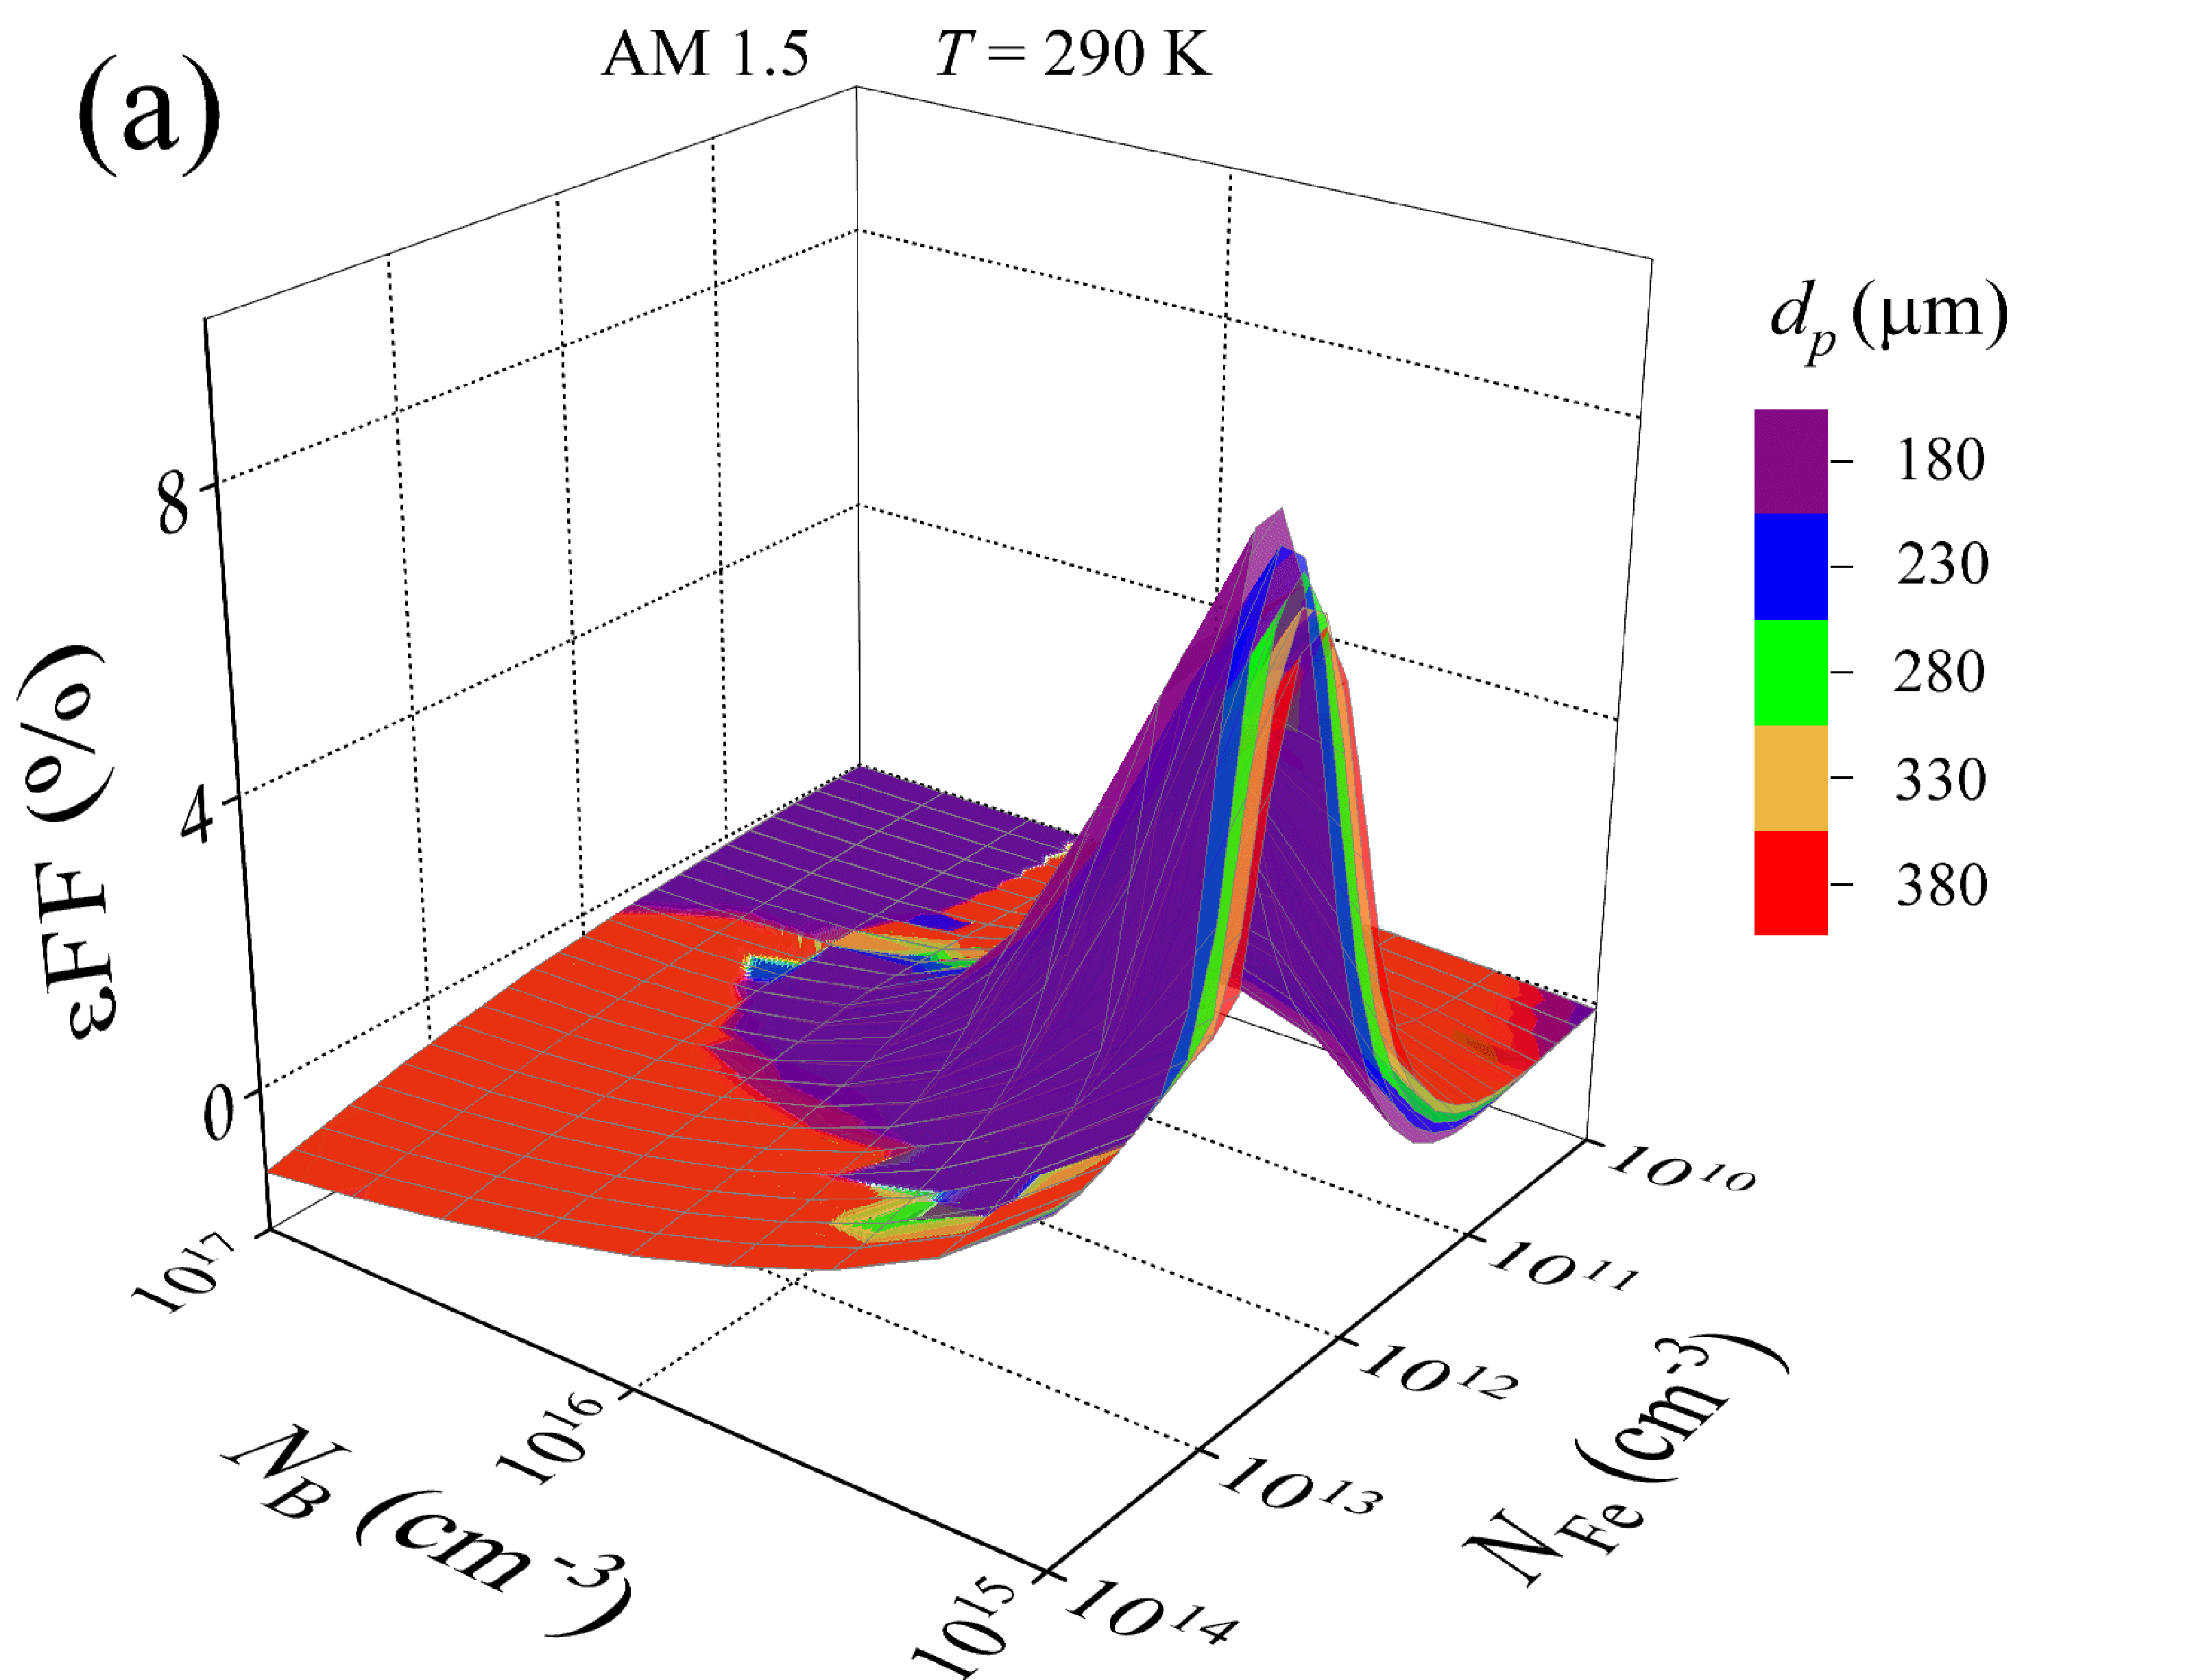
\includegraphics[width=0.49\linewidth]{Fig8a.png}
     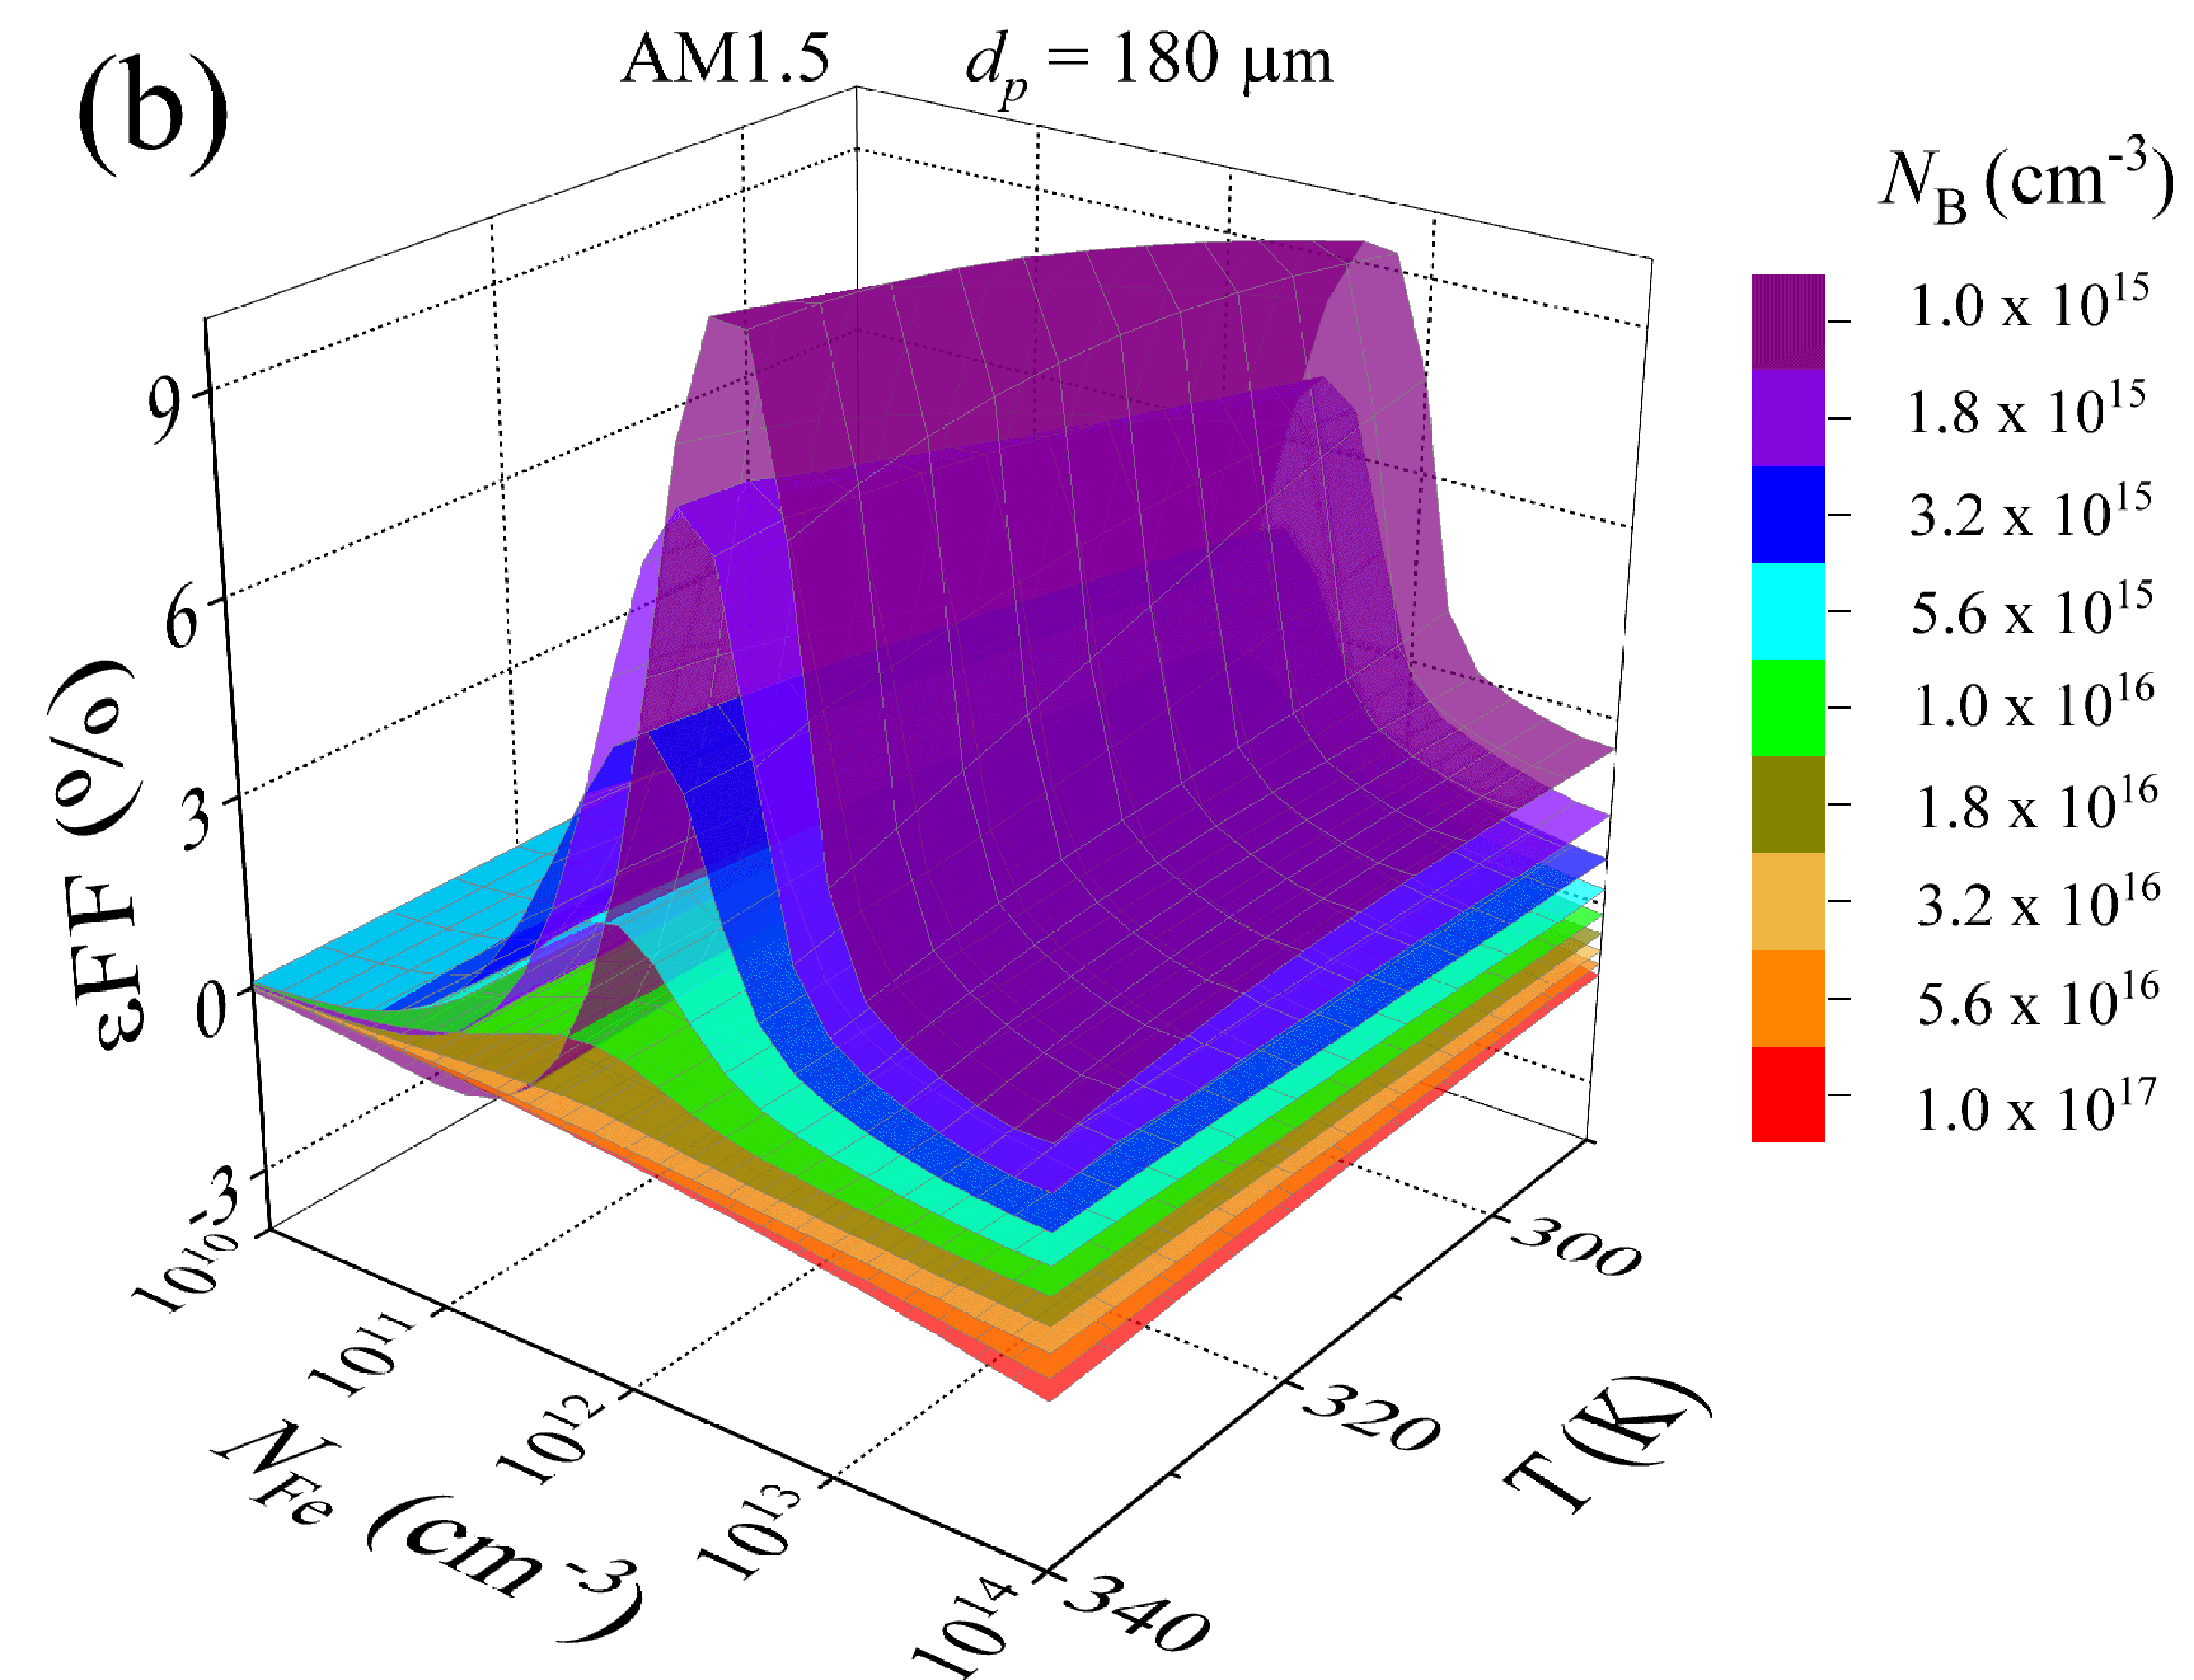
\includegraphics[width=0.49\linewidth]{Fig8b.png}
     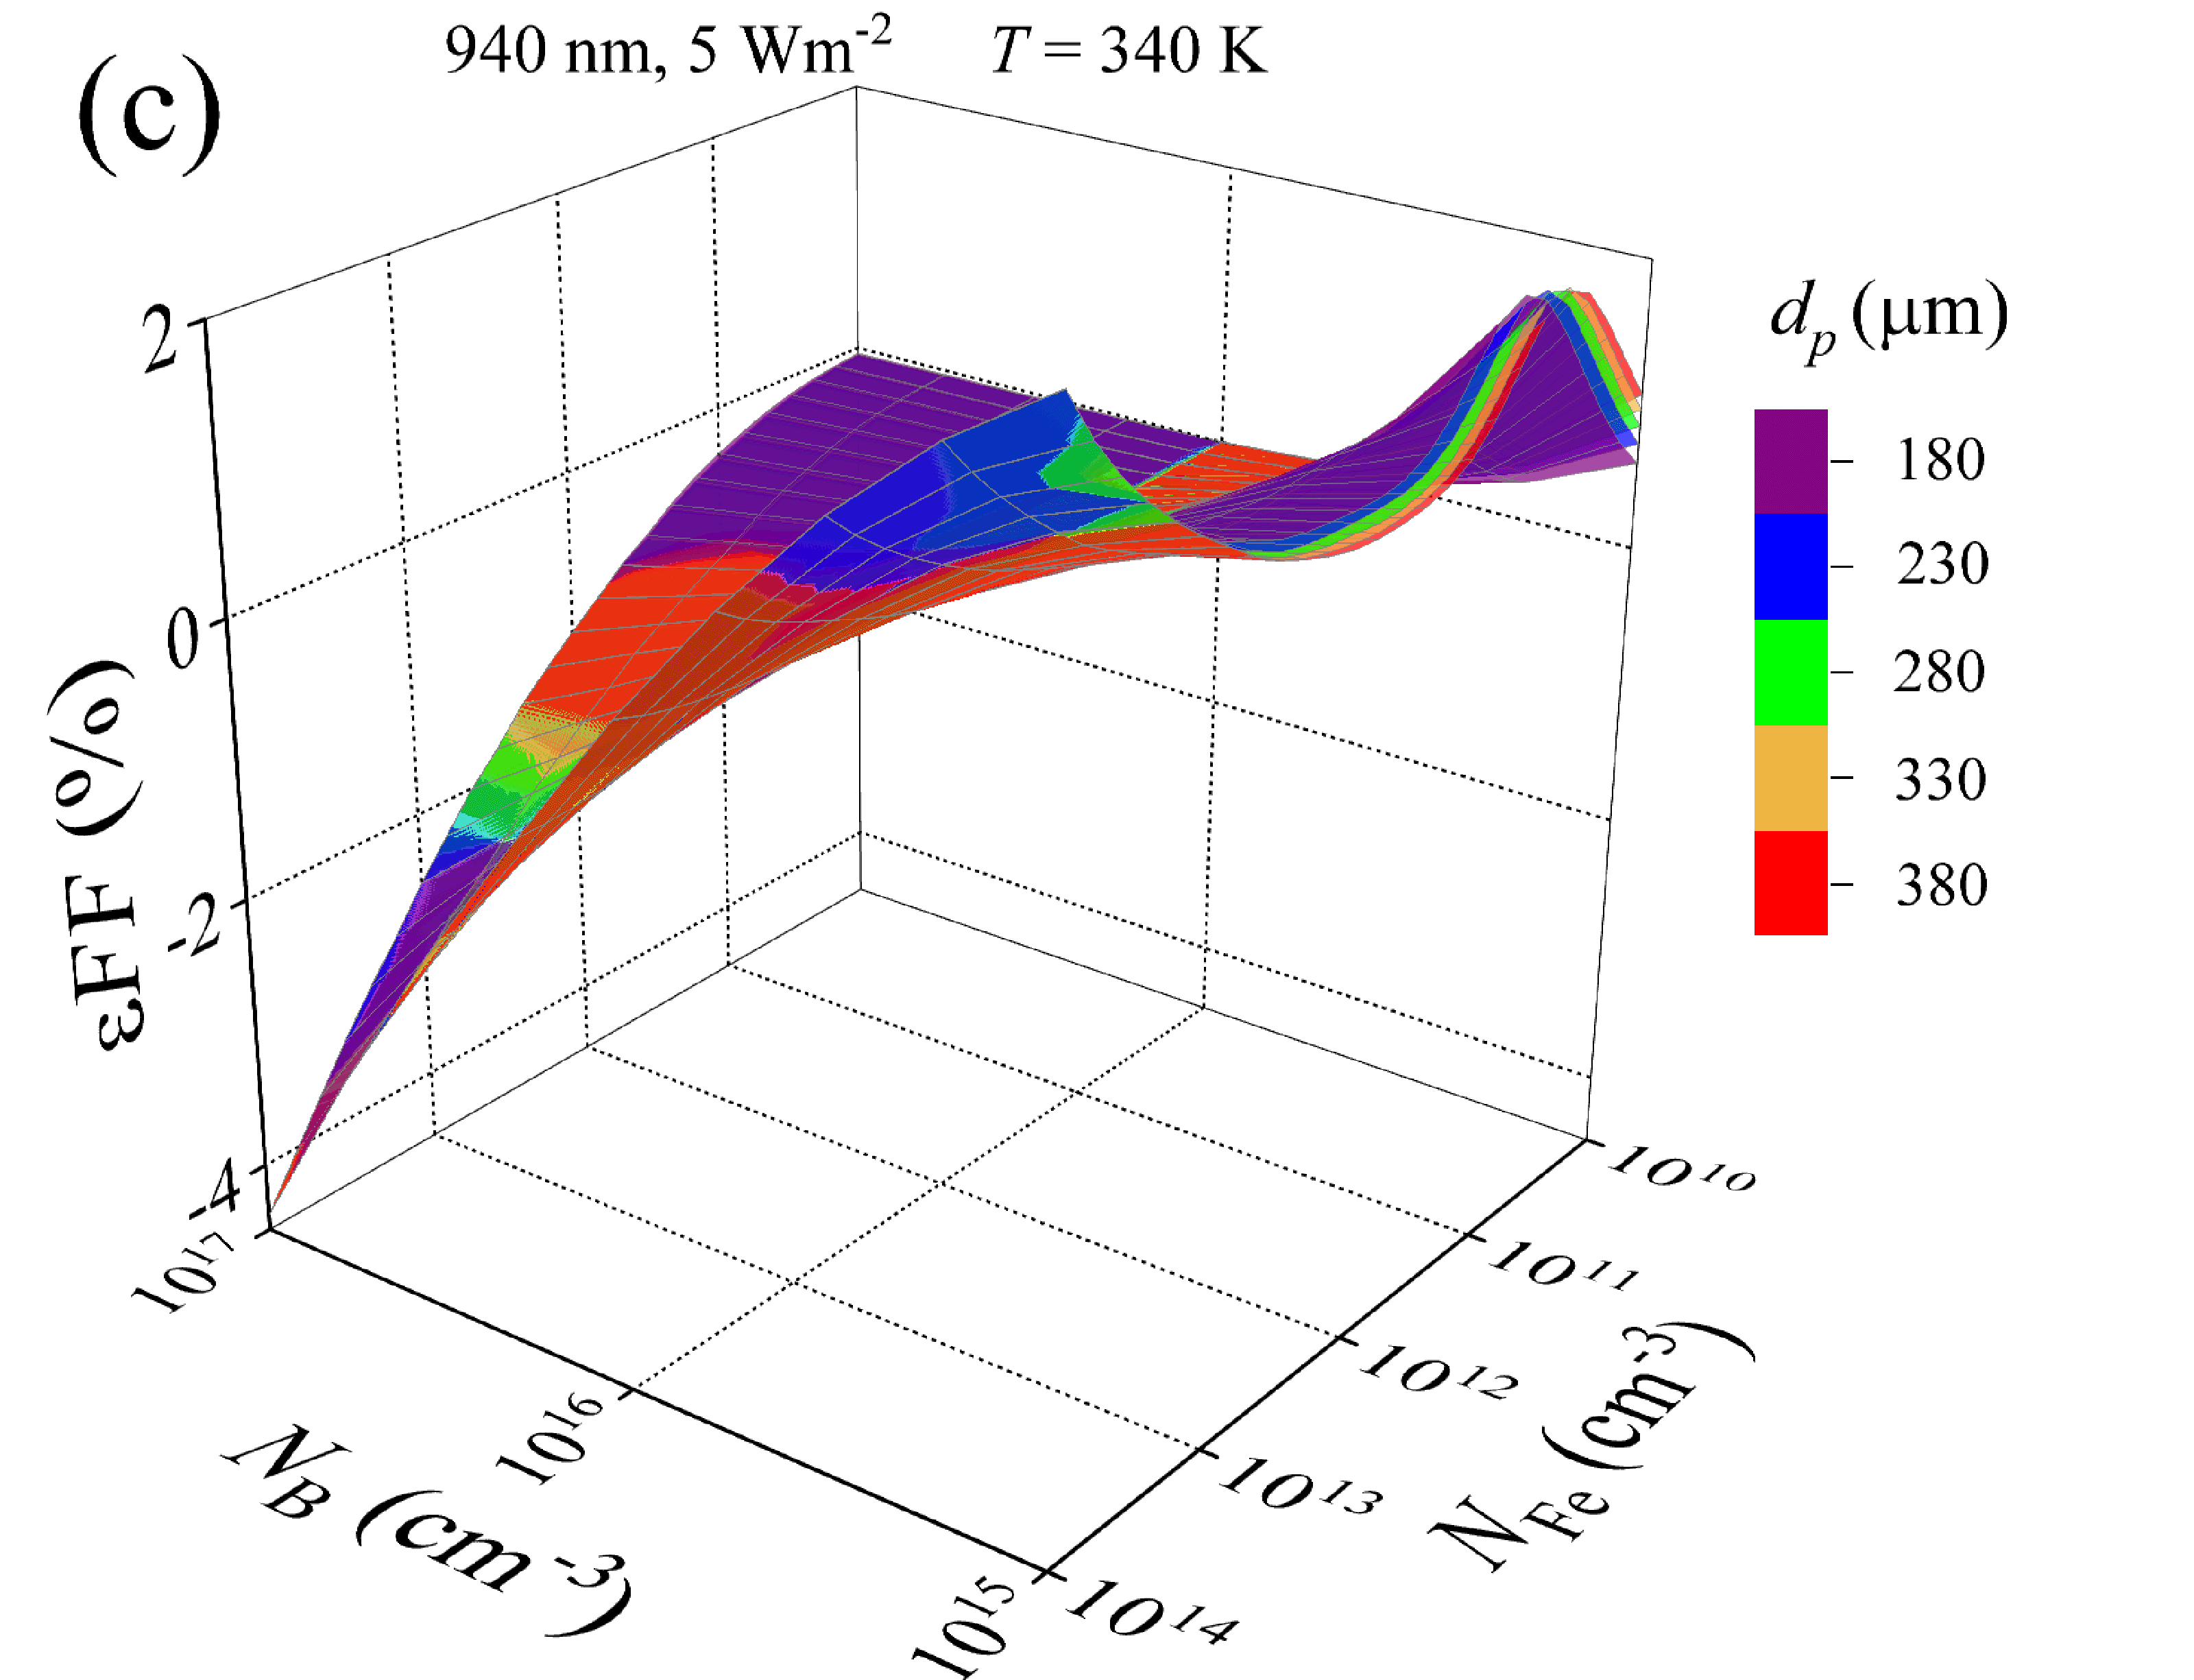
\includegraphics[width=0.49\linewidth]{Fig8c.png}
     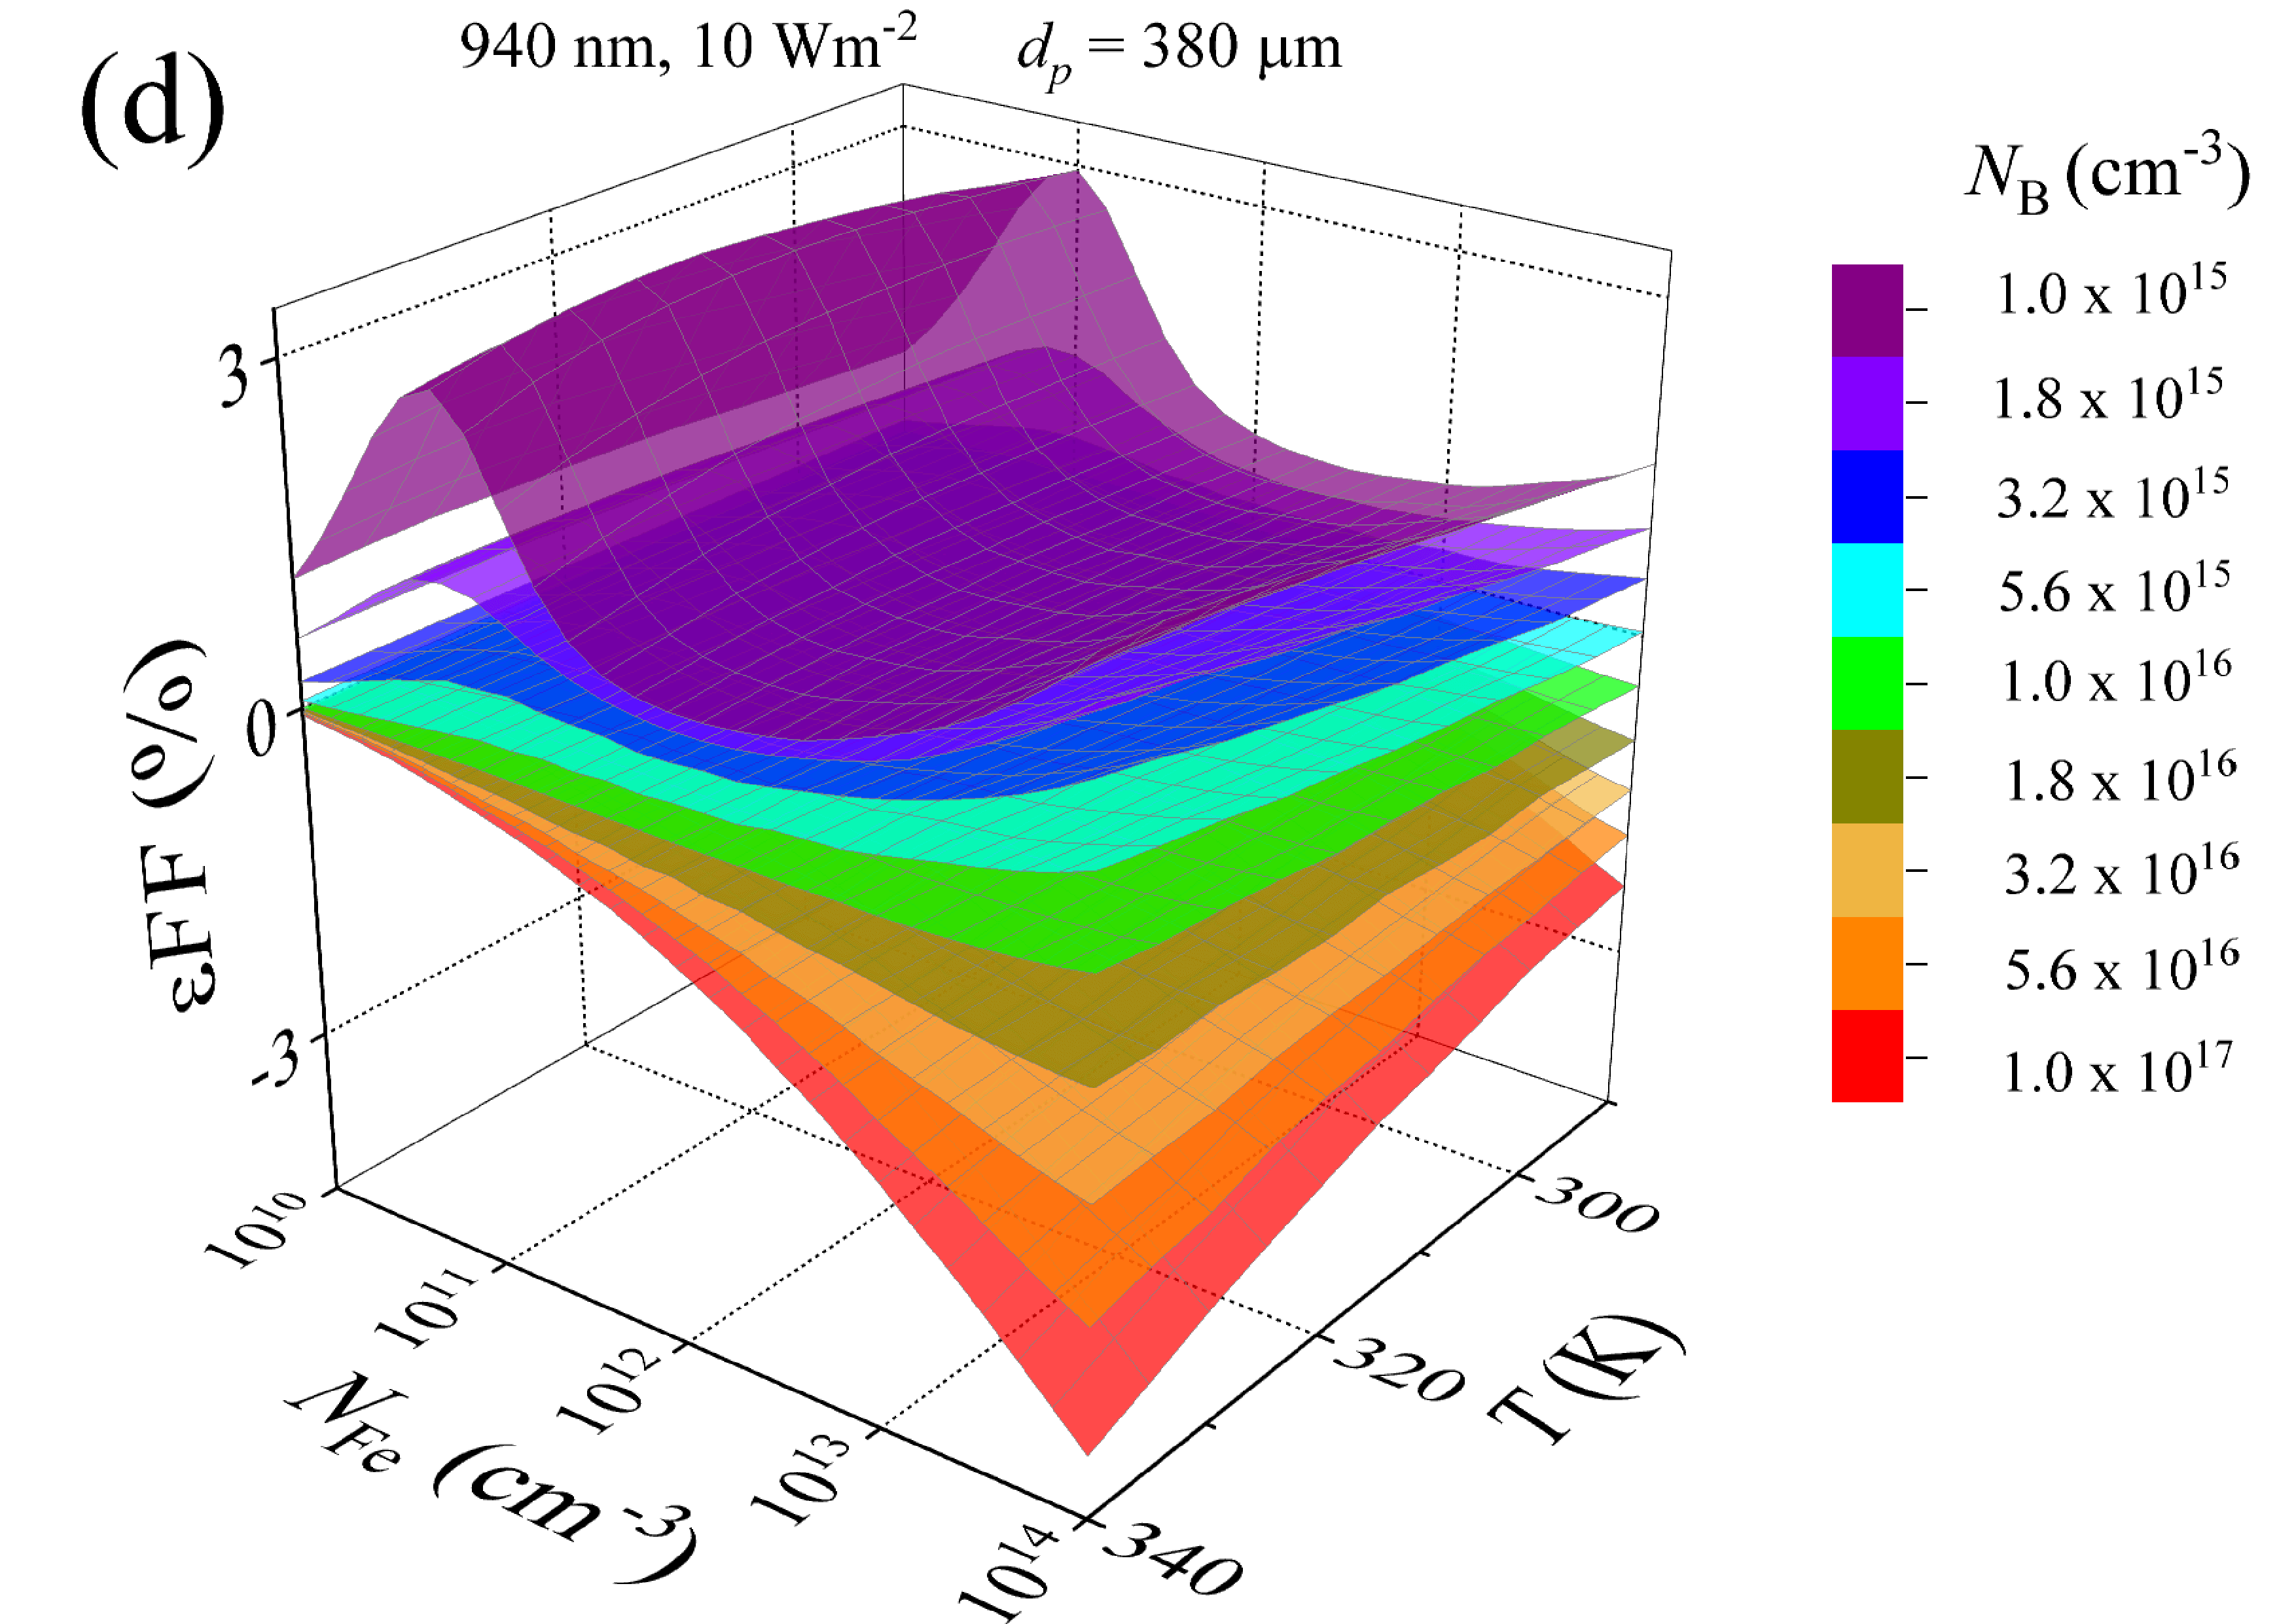
\includegraphics[width=0.49\linewidth]{Fig8d.png}
	  \caption{Relative changes in fill factor caused by a complete
       dissociation of Fe$_i$B$_s$ pairs as a function of
       iron concentration and
       doping level (panels a and c) or temperature (b, d).
       Illumination: AM1.5 (a, b), 940~nm 5~Wm$^{-2}$ (c),  940~nm 10~Wm$^{-2}$ (d).
       $T$, K: 290 (a), 340 (c).
       $d_p$, $\mu$m: 180 (b), 380 (d).
       Different surfaces correspond to different base depths (a, c) and doping levels (b, d).
}\label{fig8}
\end{figure}

\noindent
- The changes in the fill factor are the smallest among the parameters considered,
with maximum $\varepsilon F\!F$ values not exceeding 10\%;

\noindent
- At low boron concentrations ($N_\mathrm{B}<10^{16}$~cm$^{-3}$),
the dependence of $\varepsilon F\!F$ on $N_\mathrm{Fe}$ is notably non-linear.
Within the used concentration range, two regions of decrease and two regions of increase in $\varepsilon F\!F$ are observed;

\noindent
- At low boron concentrations, the change in fill factor value is positive and,
in contrast to $\varepsilon V_\mathrm{OC}$ and $\varepsilon I_\mathrm{SC}$,
AM1.5 illumination causes more significant changes in $\varepsilon F\!F$ than monochromatic illumination.
At high boron concentrations, the $\varepsilon F\!F$ is negative and does not exceed 4\%;


\noindent
- The absolute value of $\varepsilon F\!F$ increases, regardless of the value sign, with temperature increases;


\noindent
- Increasing the base thickness leads to a decrease in $\varepsilon F\!F$ (a reduction in the fill factor with increasing $d_p$ is expected according to (\ref{eqFF3})). Additionally, this results in a shift of the $\varepsilon F\!F\left(N_\mathrm{Fe}\right)$ dependence towards lower iron concentrations.
The impact of $d_p$ is more pronounced at low boron concentrations and in the case of AM1.5 illumination;


\noindent
- In the case of monochromatic illumination, the light intensity significantly affects the relative changes in the fill factor
($\varepsilon F\!F$ can vary by a factor of 2 when $W_\mathrm{ill}$ changes from 5 to 10~Wm$^{-2}$).
This impact is influenced by both iron concentration (which can even change the sign of the effect) and temperature.

Fig.~\ref{fig9} shows that the experimental dependencies of  $\varepsilon F\!F\left(N_\mathrm{Fe}\right)$
and $\varepsilon F\!F\left(T\right)$ align well with the calculated values.

Figure~\ref{fig9} shows that the experimental dependencies $\varepsilon F\!F$$\left(N_\mathrm{Fe}\right)$ and $\varepsilon F\!F$$\left(T\right)$ are in good agreement with the calculated values.
In our opinion, the quantitative agreement is limited by the relatively low accuracy of $\varepsilon F\!F$ measurements
and the dependence of fill factor on series and shunt resistances \cite{Green1981,Green1982},
which were not considered in the simulation.


\begin{figure}
	\centering
     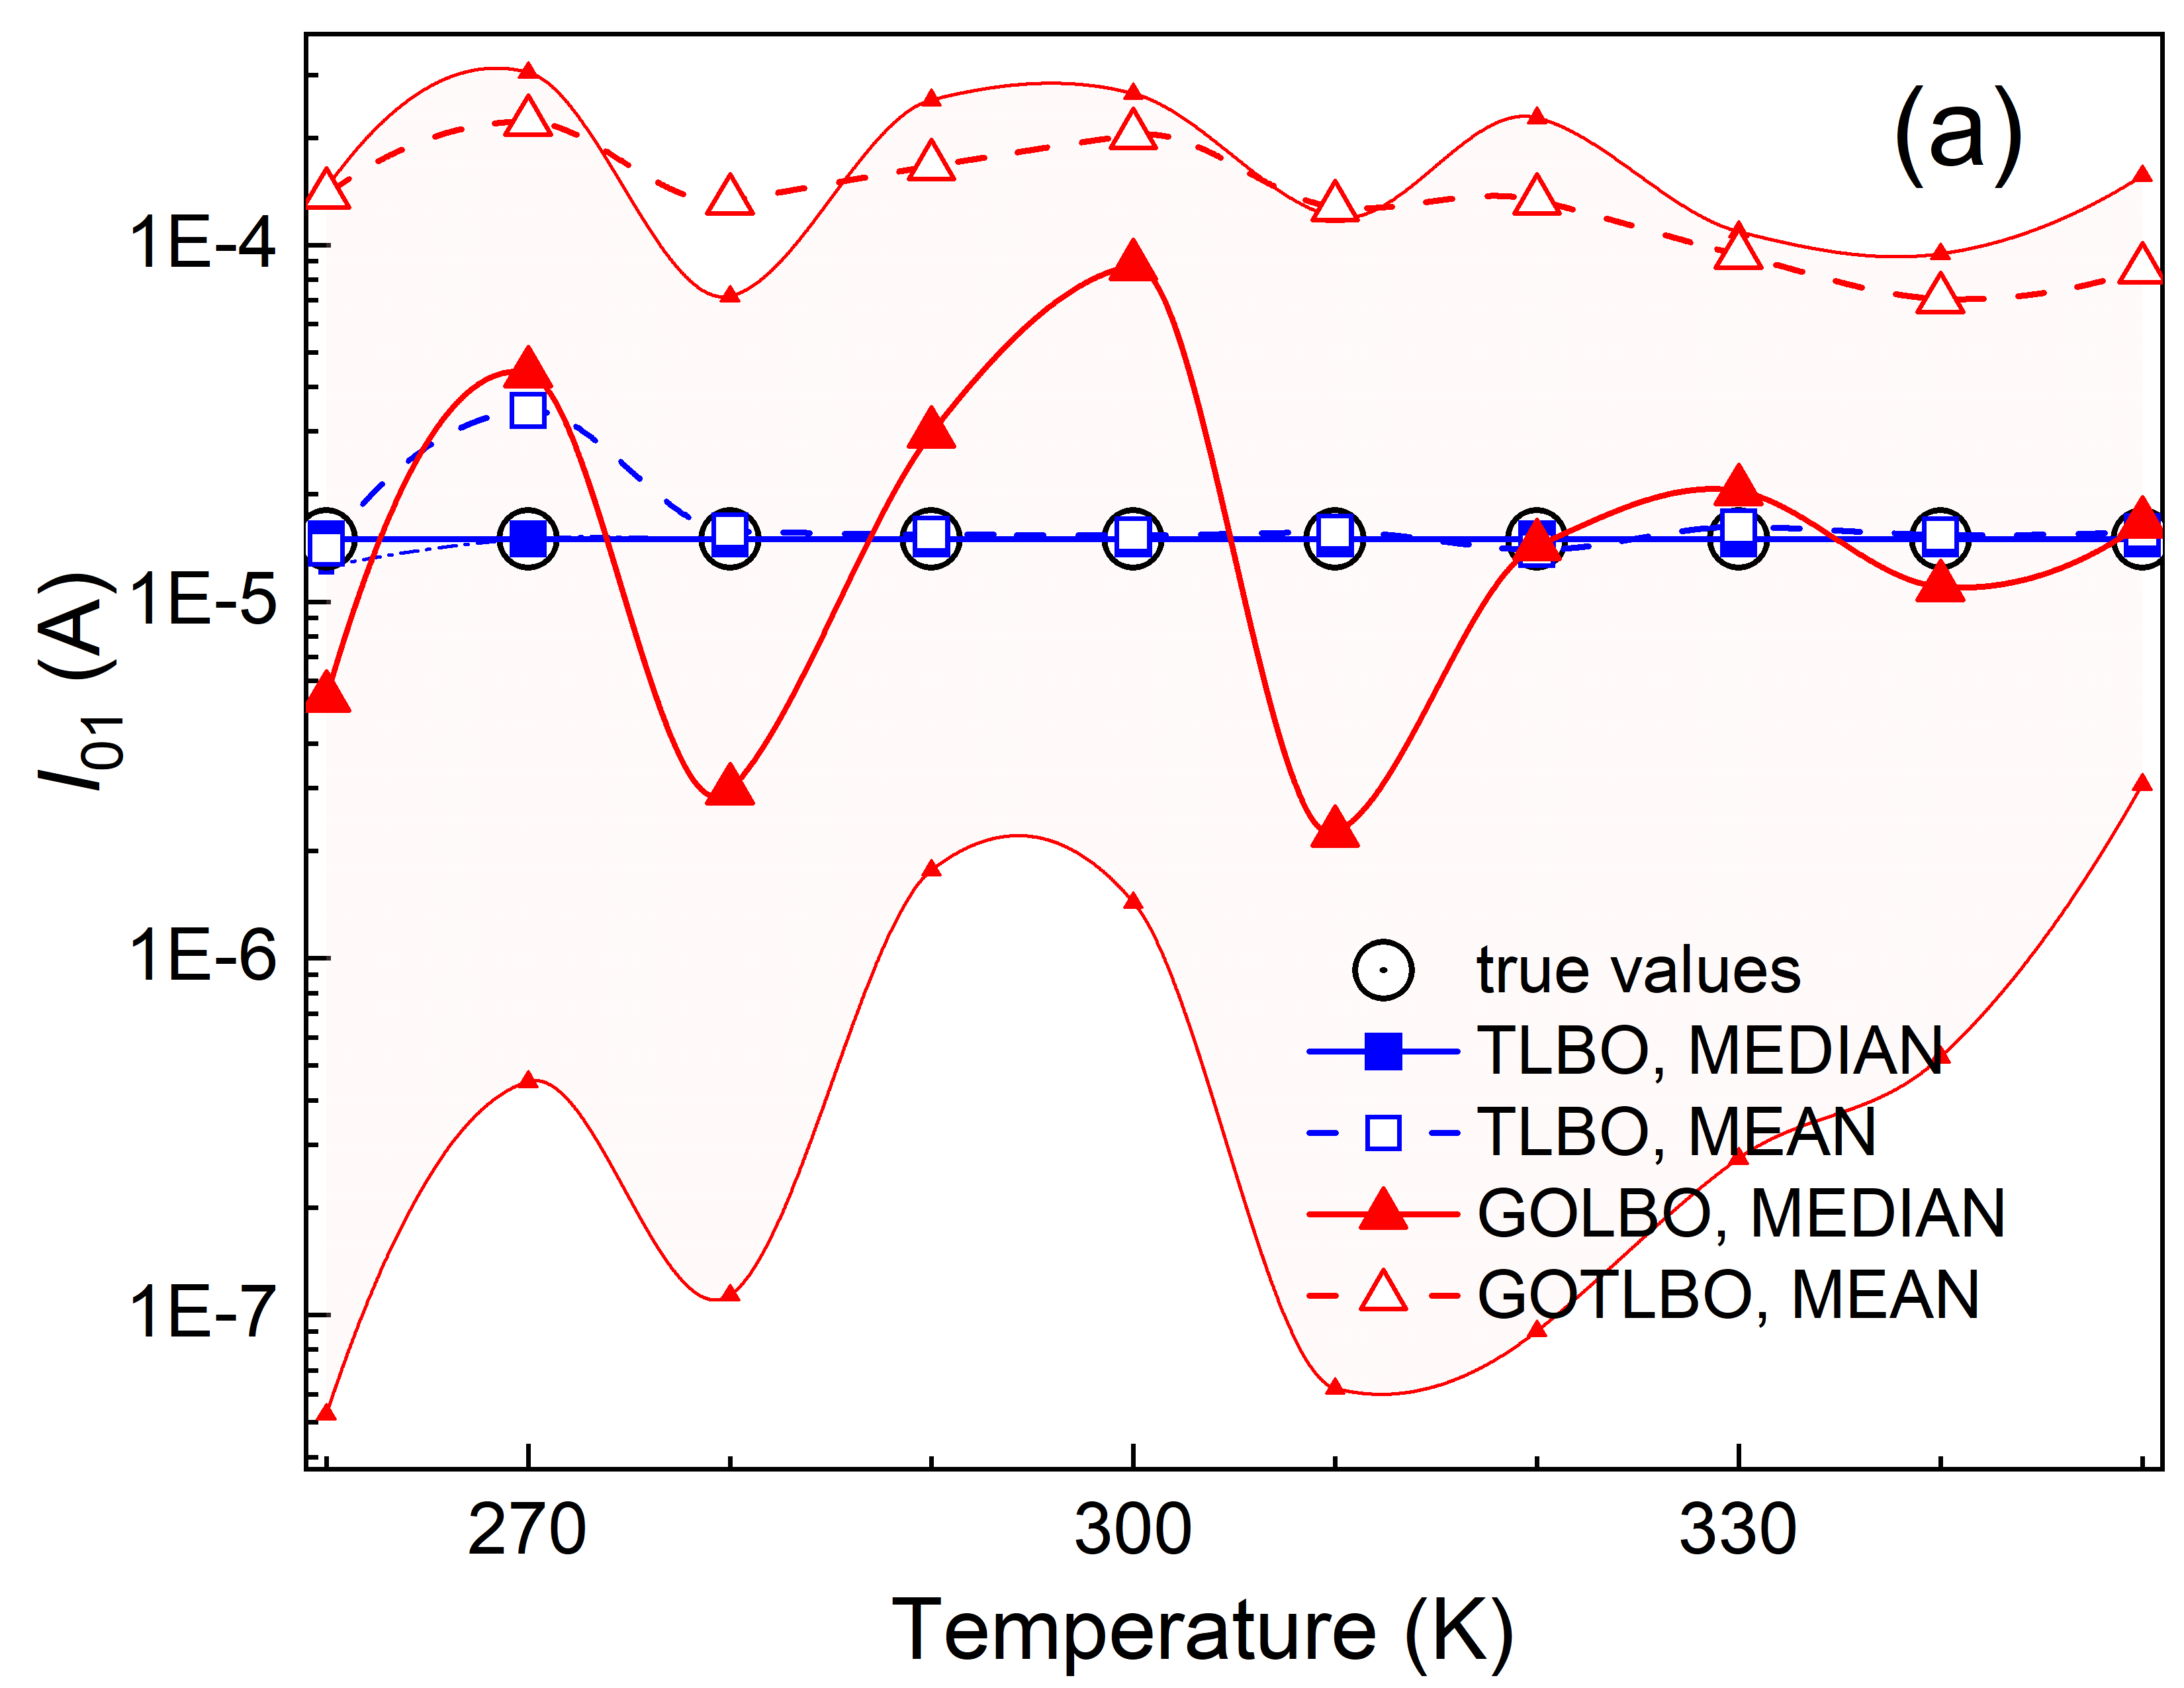
\includegraphics[width=0.4\linewidth]{Fig9a.png}
     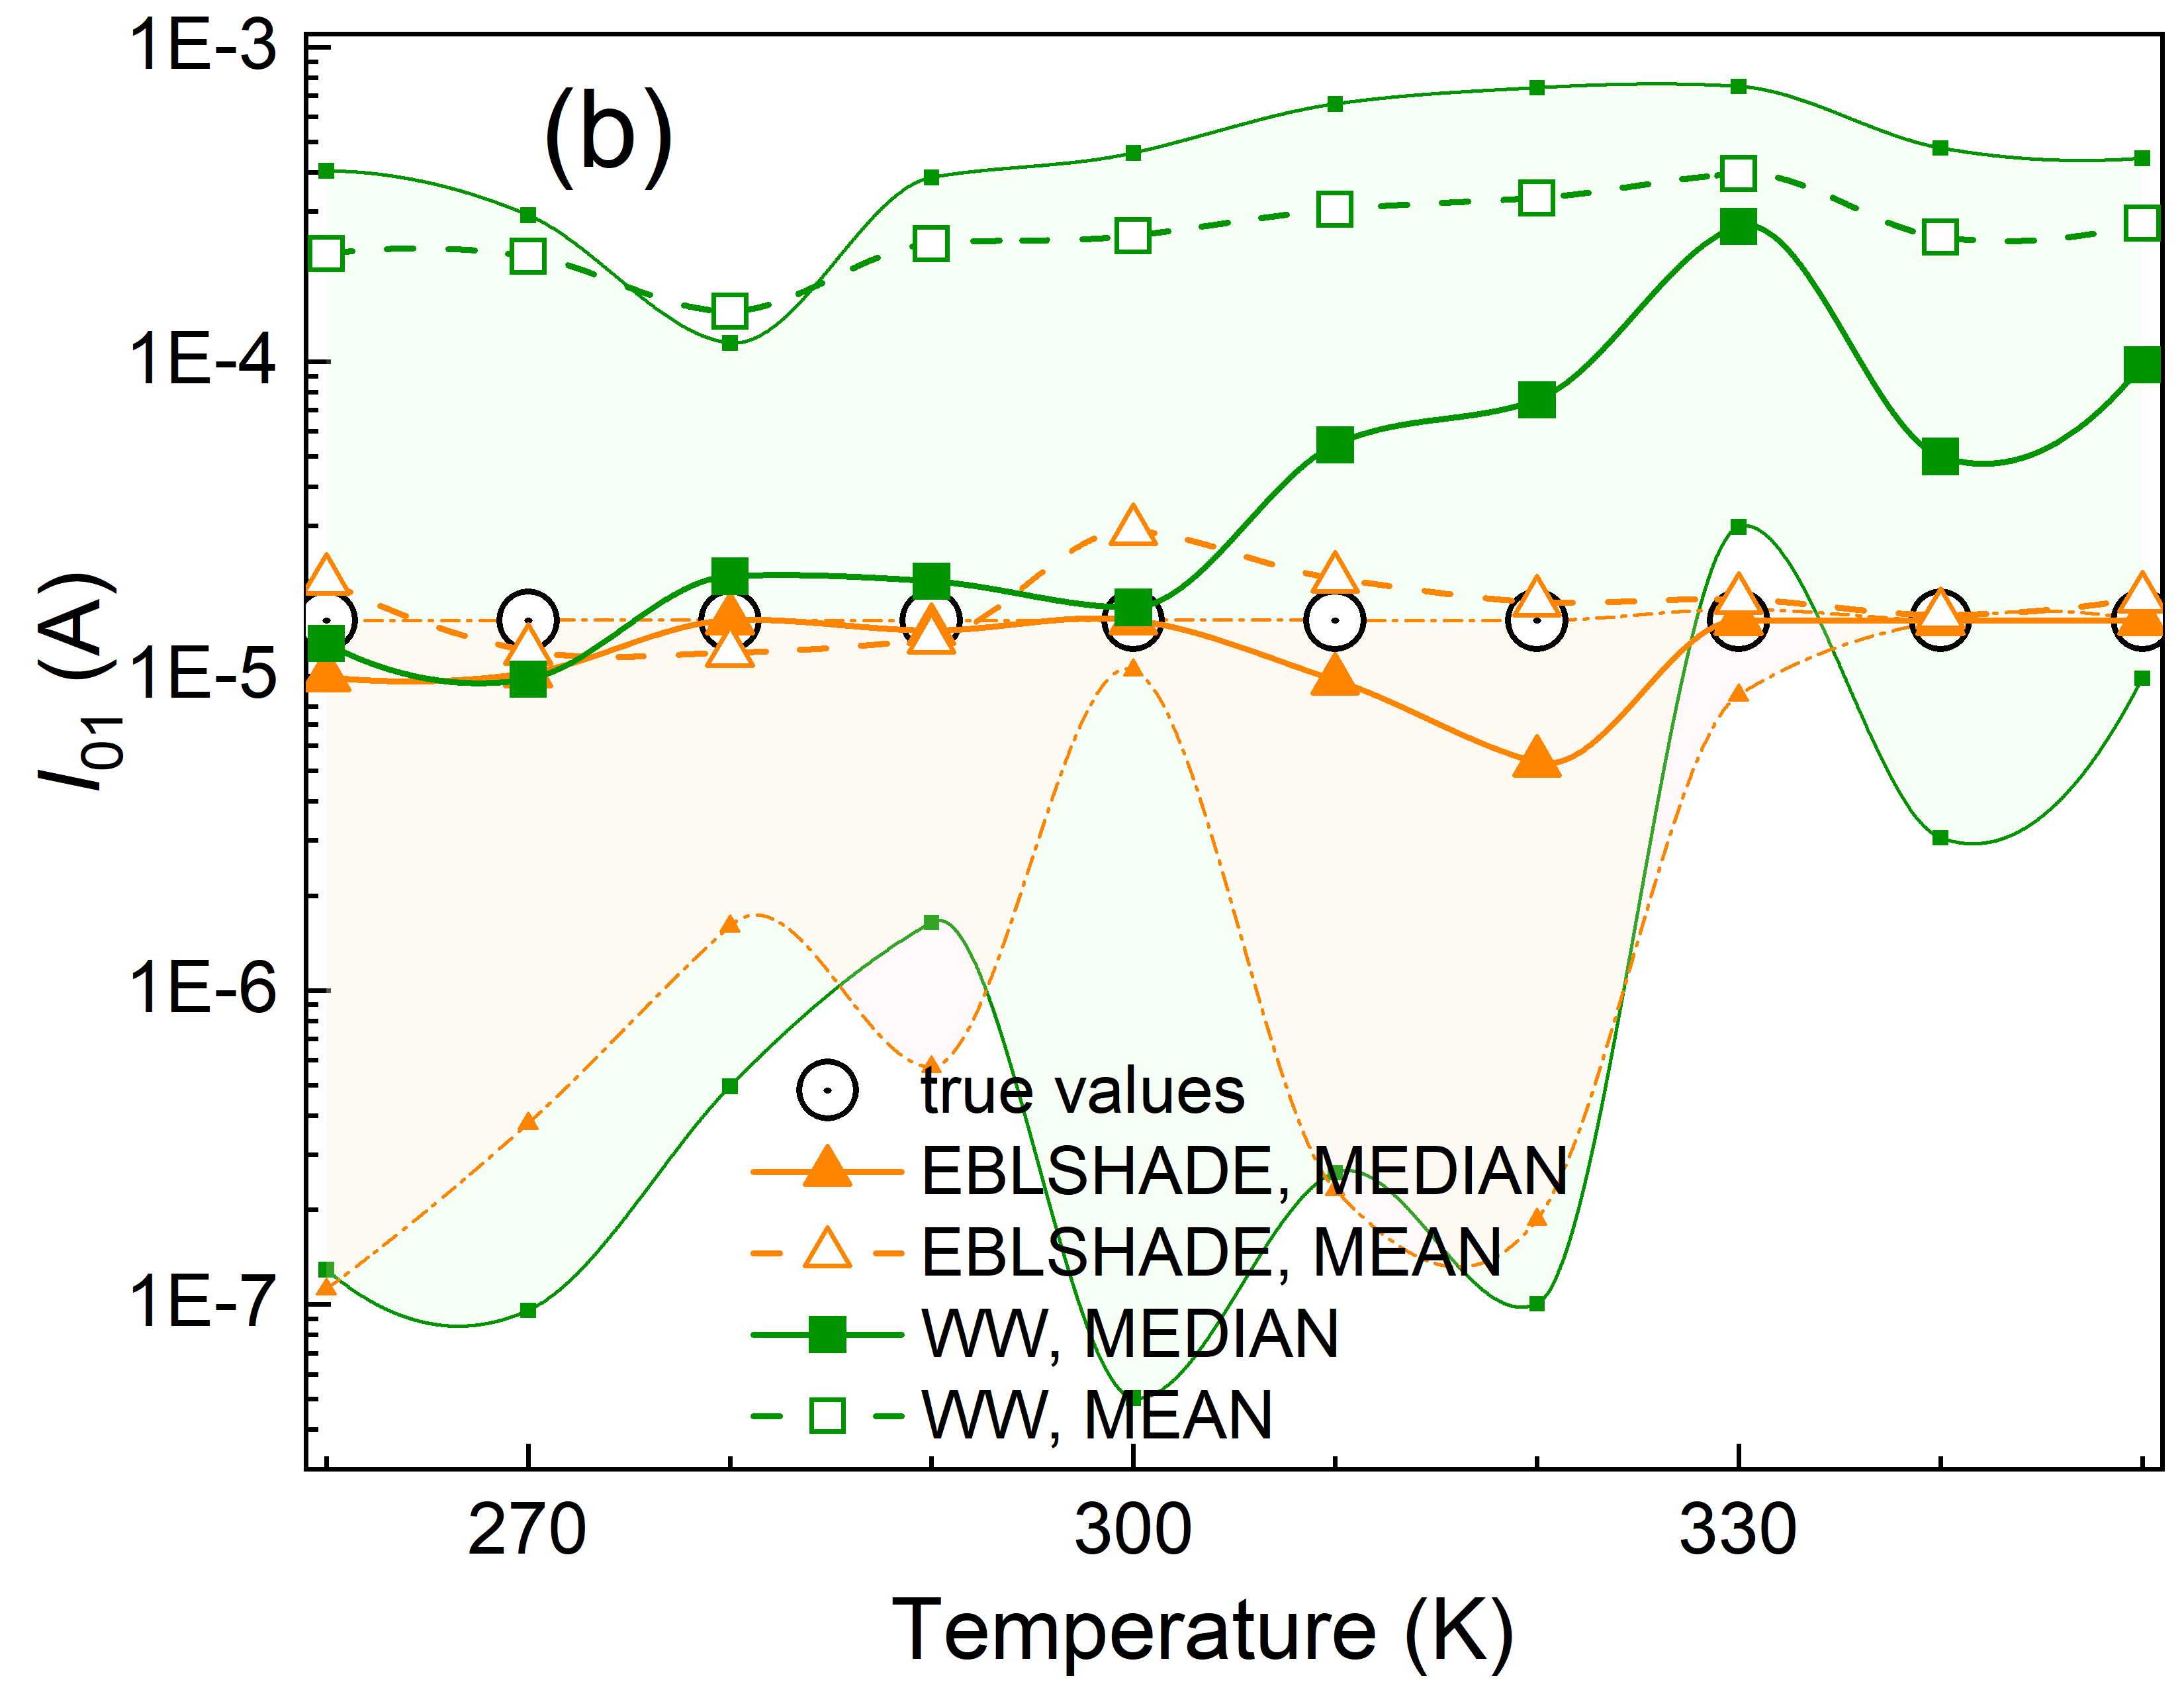
\includegraphics[width=0.4\linewidth]{Fig9b.png}
	  \caption{Relative changes in fill factor caused by a complete
       dissociation of Fe$_i$B$_s$ pairs as a function of iron concentration (a) and
       temperature (b) for SSC with $d_p=380$~$\mu$m and $N_\mathrm{B}=1.36\times10^{15}$~cm$^{-3}$
       in the case of monochromatic (940~nm) illumination.
       The marks are the experimental results, the lines are the simulation results.
       $W_\mathrm{ill}$, Wm$^{-2}$: 5 (marks and solid lines), 10 (dotted lines).
       Different lines and marks correspond to different temperatures (a) or $N_\mathrm{Fe}$ values (b) --- see legends.
}\label{fig9}
\end{figure}

The observed characteristics of $\varepsilon F\!F$ suggest that
the fill factor is considerably less suitable for estimating iron concentration in SSCs
than the short-circuit current and open-circuit voltage.
$\varepsilon F\!F$ can serve as an auxiliary parameter to refine $N_\mathrm{Fe}$;
however, if monochromatic illumination is used, light intensity must be controlled with high precision.



\subsection{Solar Cell Efficiency}

Solar cell efficiency depends on all the photovoltaic conversion parameters previously discussed:
\begin{equation}
\label{eq11}
    \eta = \frac{I_\mathrm{SC}V_\mathrm{OC}F\!F}{W_\mathrm{ill}A}\,,
\end{equation}
where
$A$ is the illuminated area of the solar cell.
Considering the differential of Eq.~(\ref{eq11}), a cumulative effect on the relative changes in efficiency can be anticipated.

Considering the differential of formula (\ref{eq11}):
\begin{equation}
\label{eq12}
    d\eta = \frac{dI_\mathrm{SC}}{I_\mathrm{SC}}+\frac{dV_\mathrm{OC}}{V_\mathrm{OC}}+\frac{dF\!F}{F\!F},
\end{equation}
a cumulative effect on the relative changes in efficiency can be anticipated.
Fig.~\ref{fig10} illustrates the simulation results for the solar cell efficiency,
while Figs.~S17–S20 offer additional details in the Supplementary Material.


\begin{figure}
	\centering
     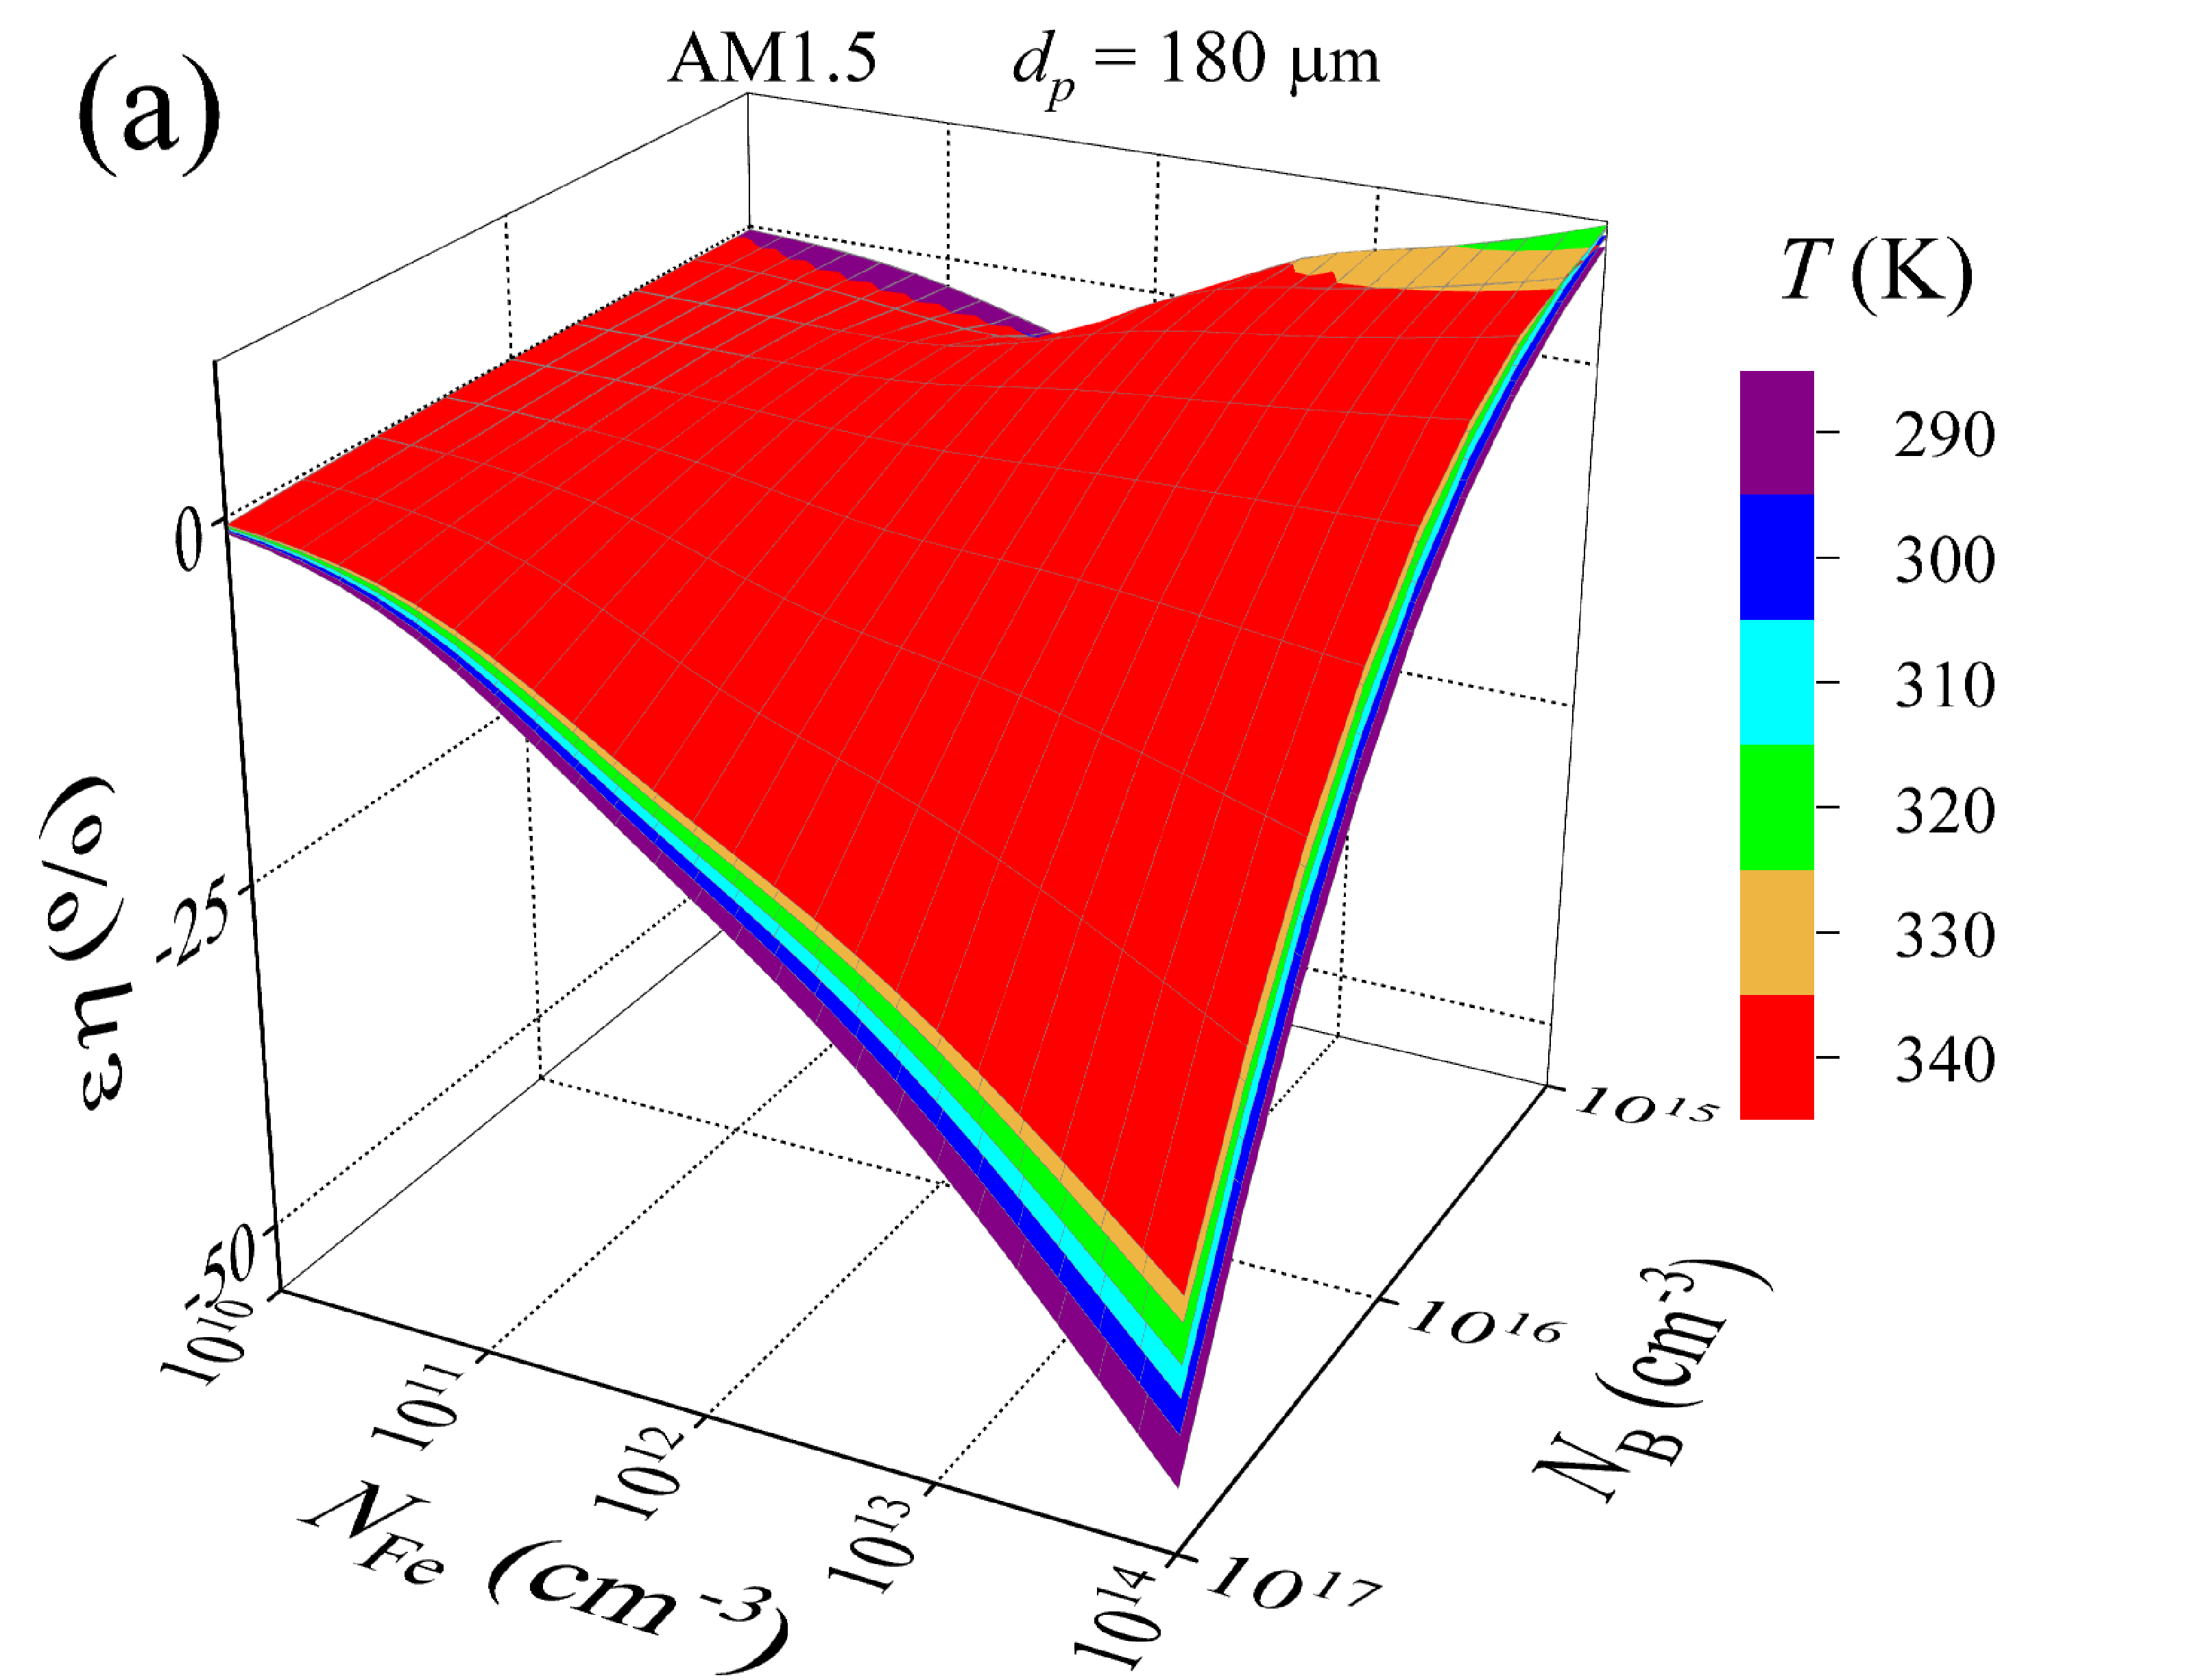
\includegraphics[width=0.49\linewidth]{Fig10a.png}
     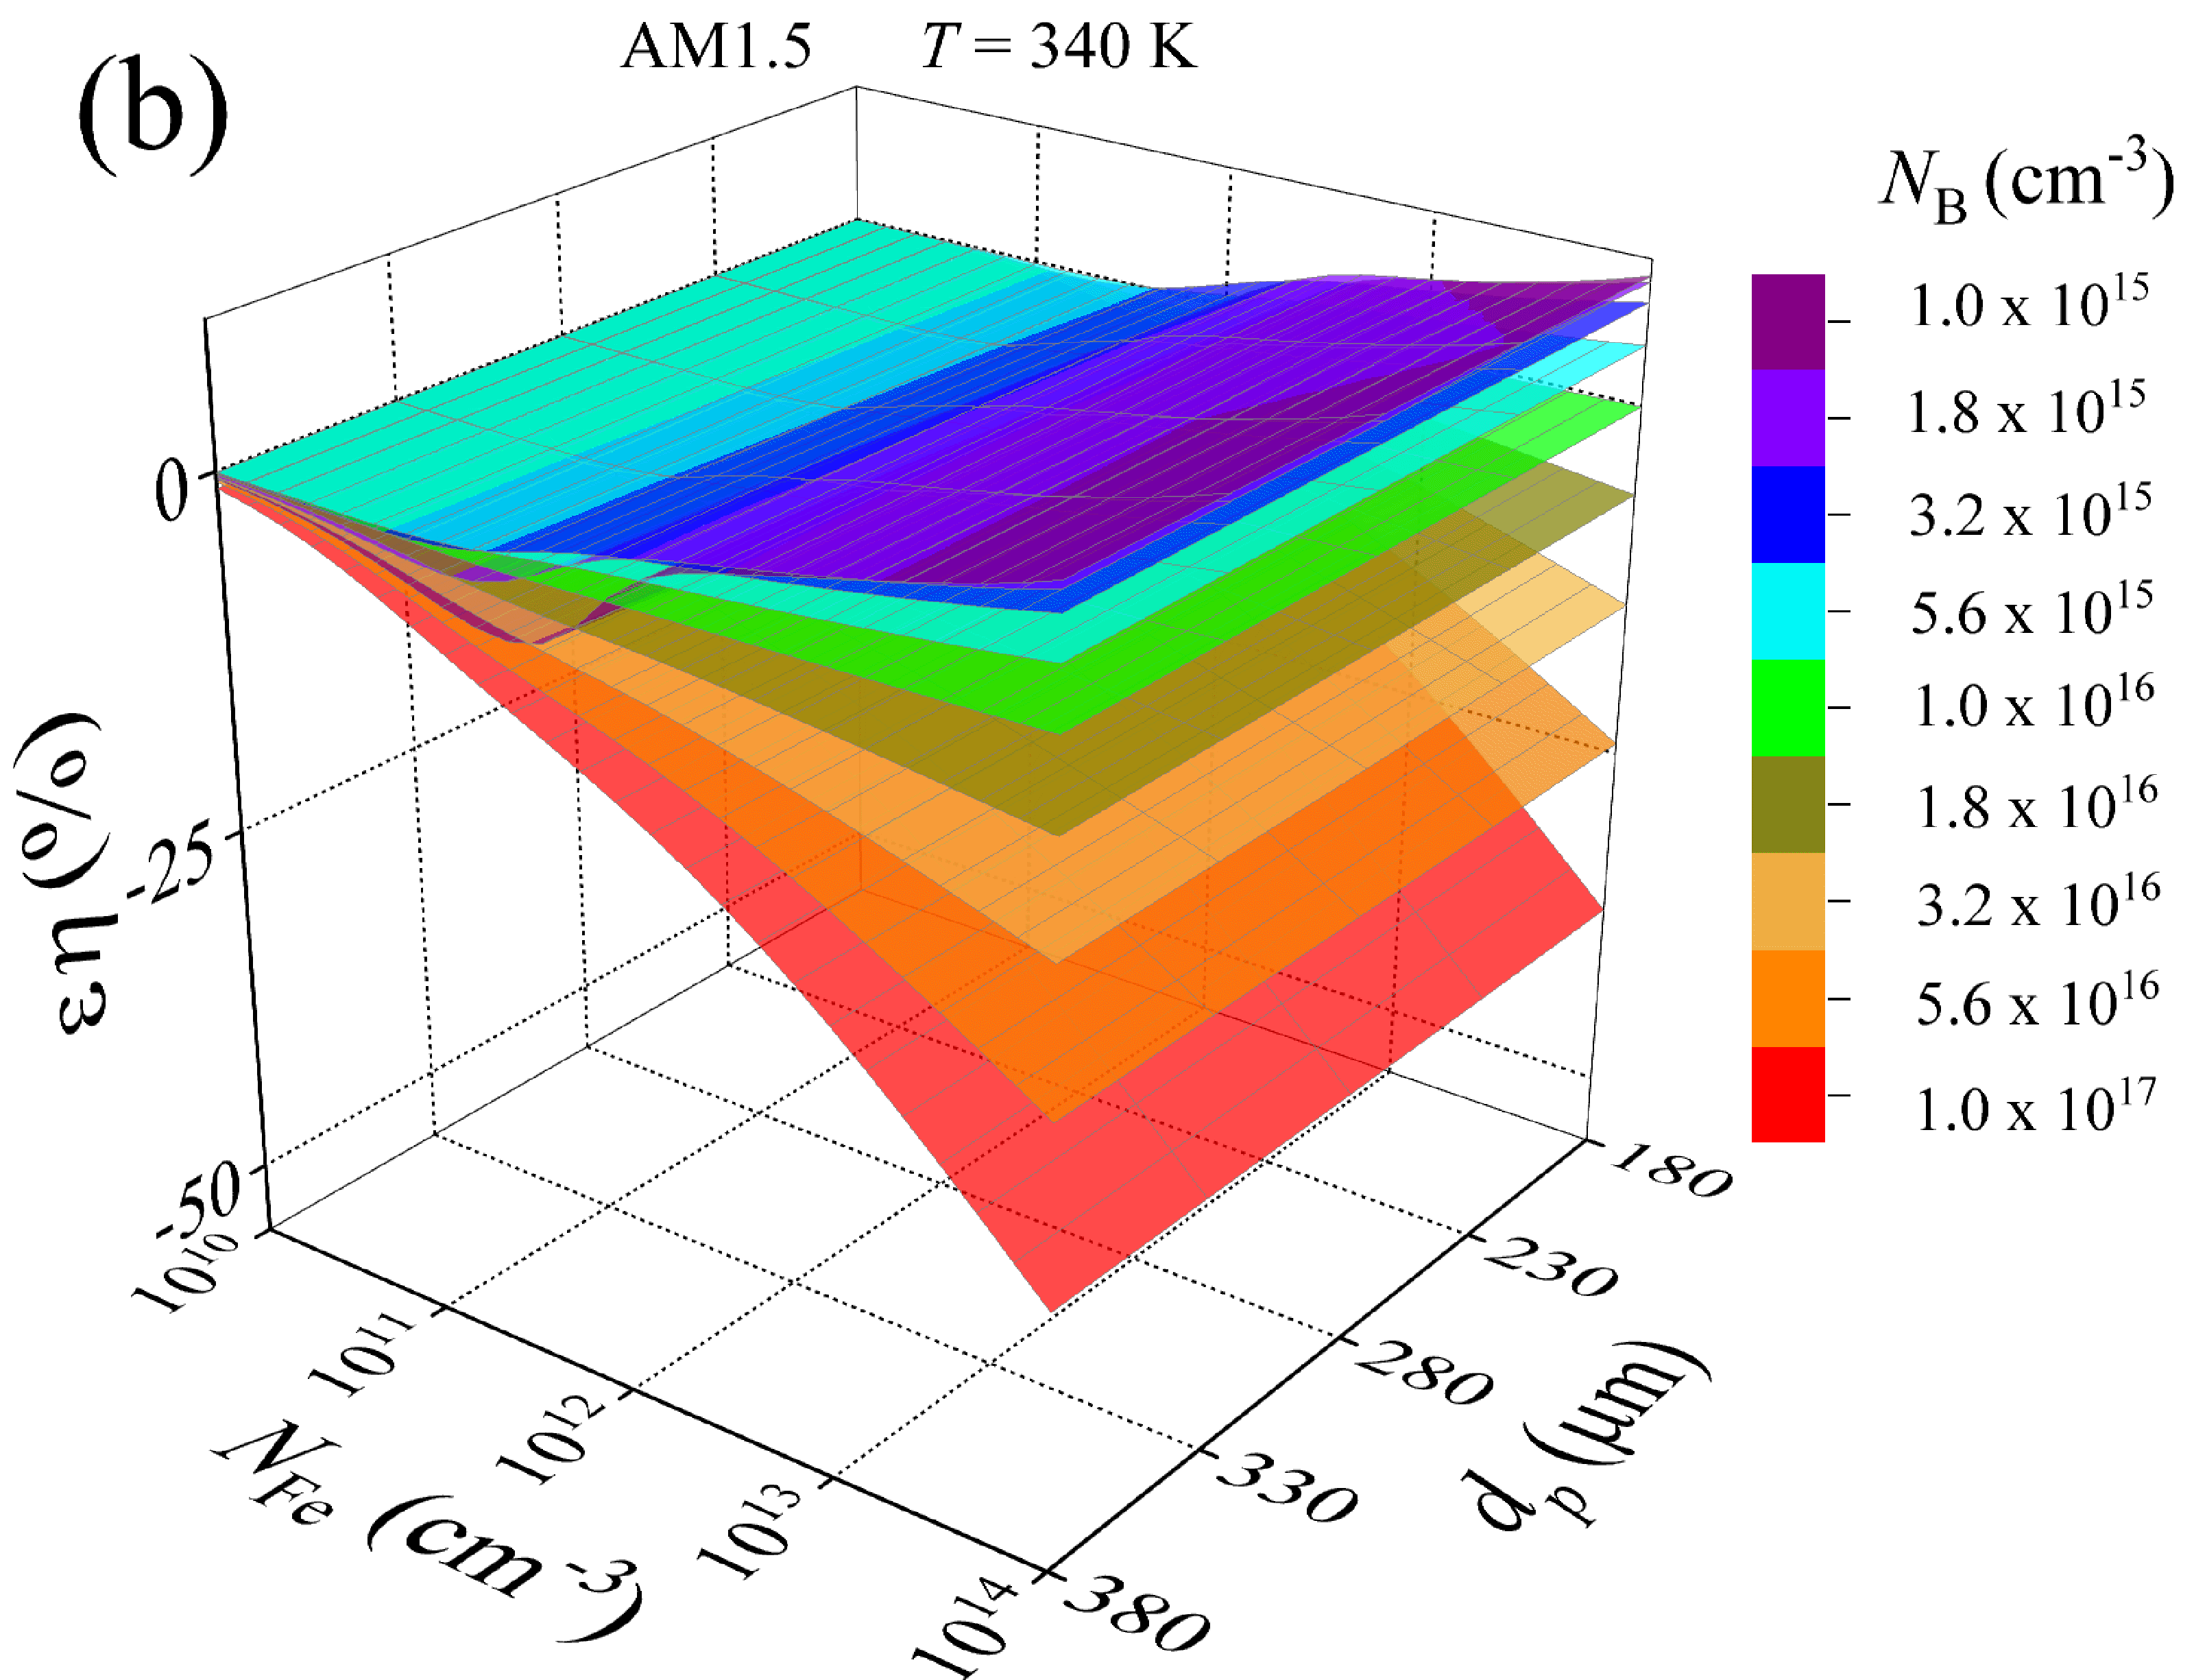
\includegraphics[width=0.49\linewidth]{Fig10b.png}
     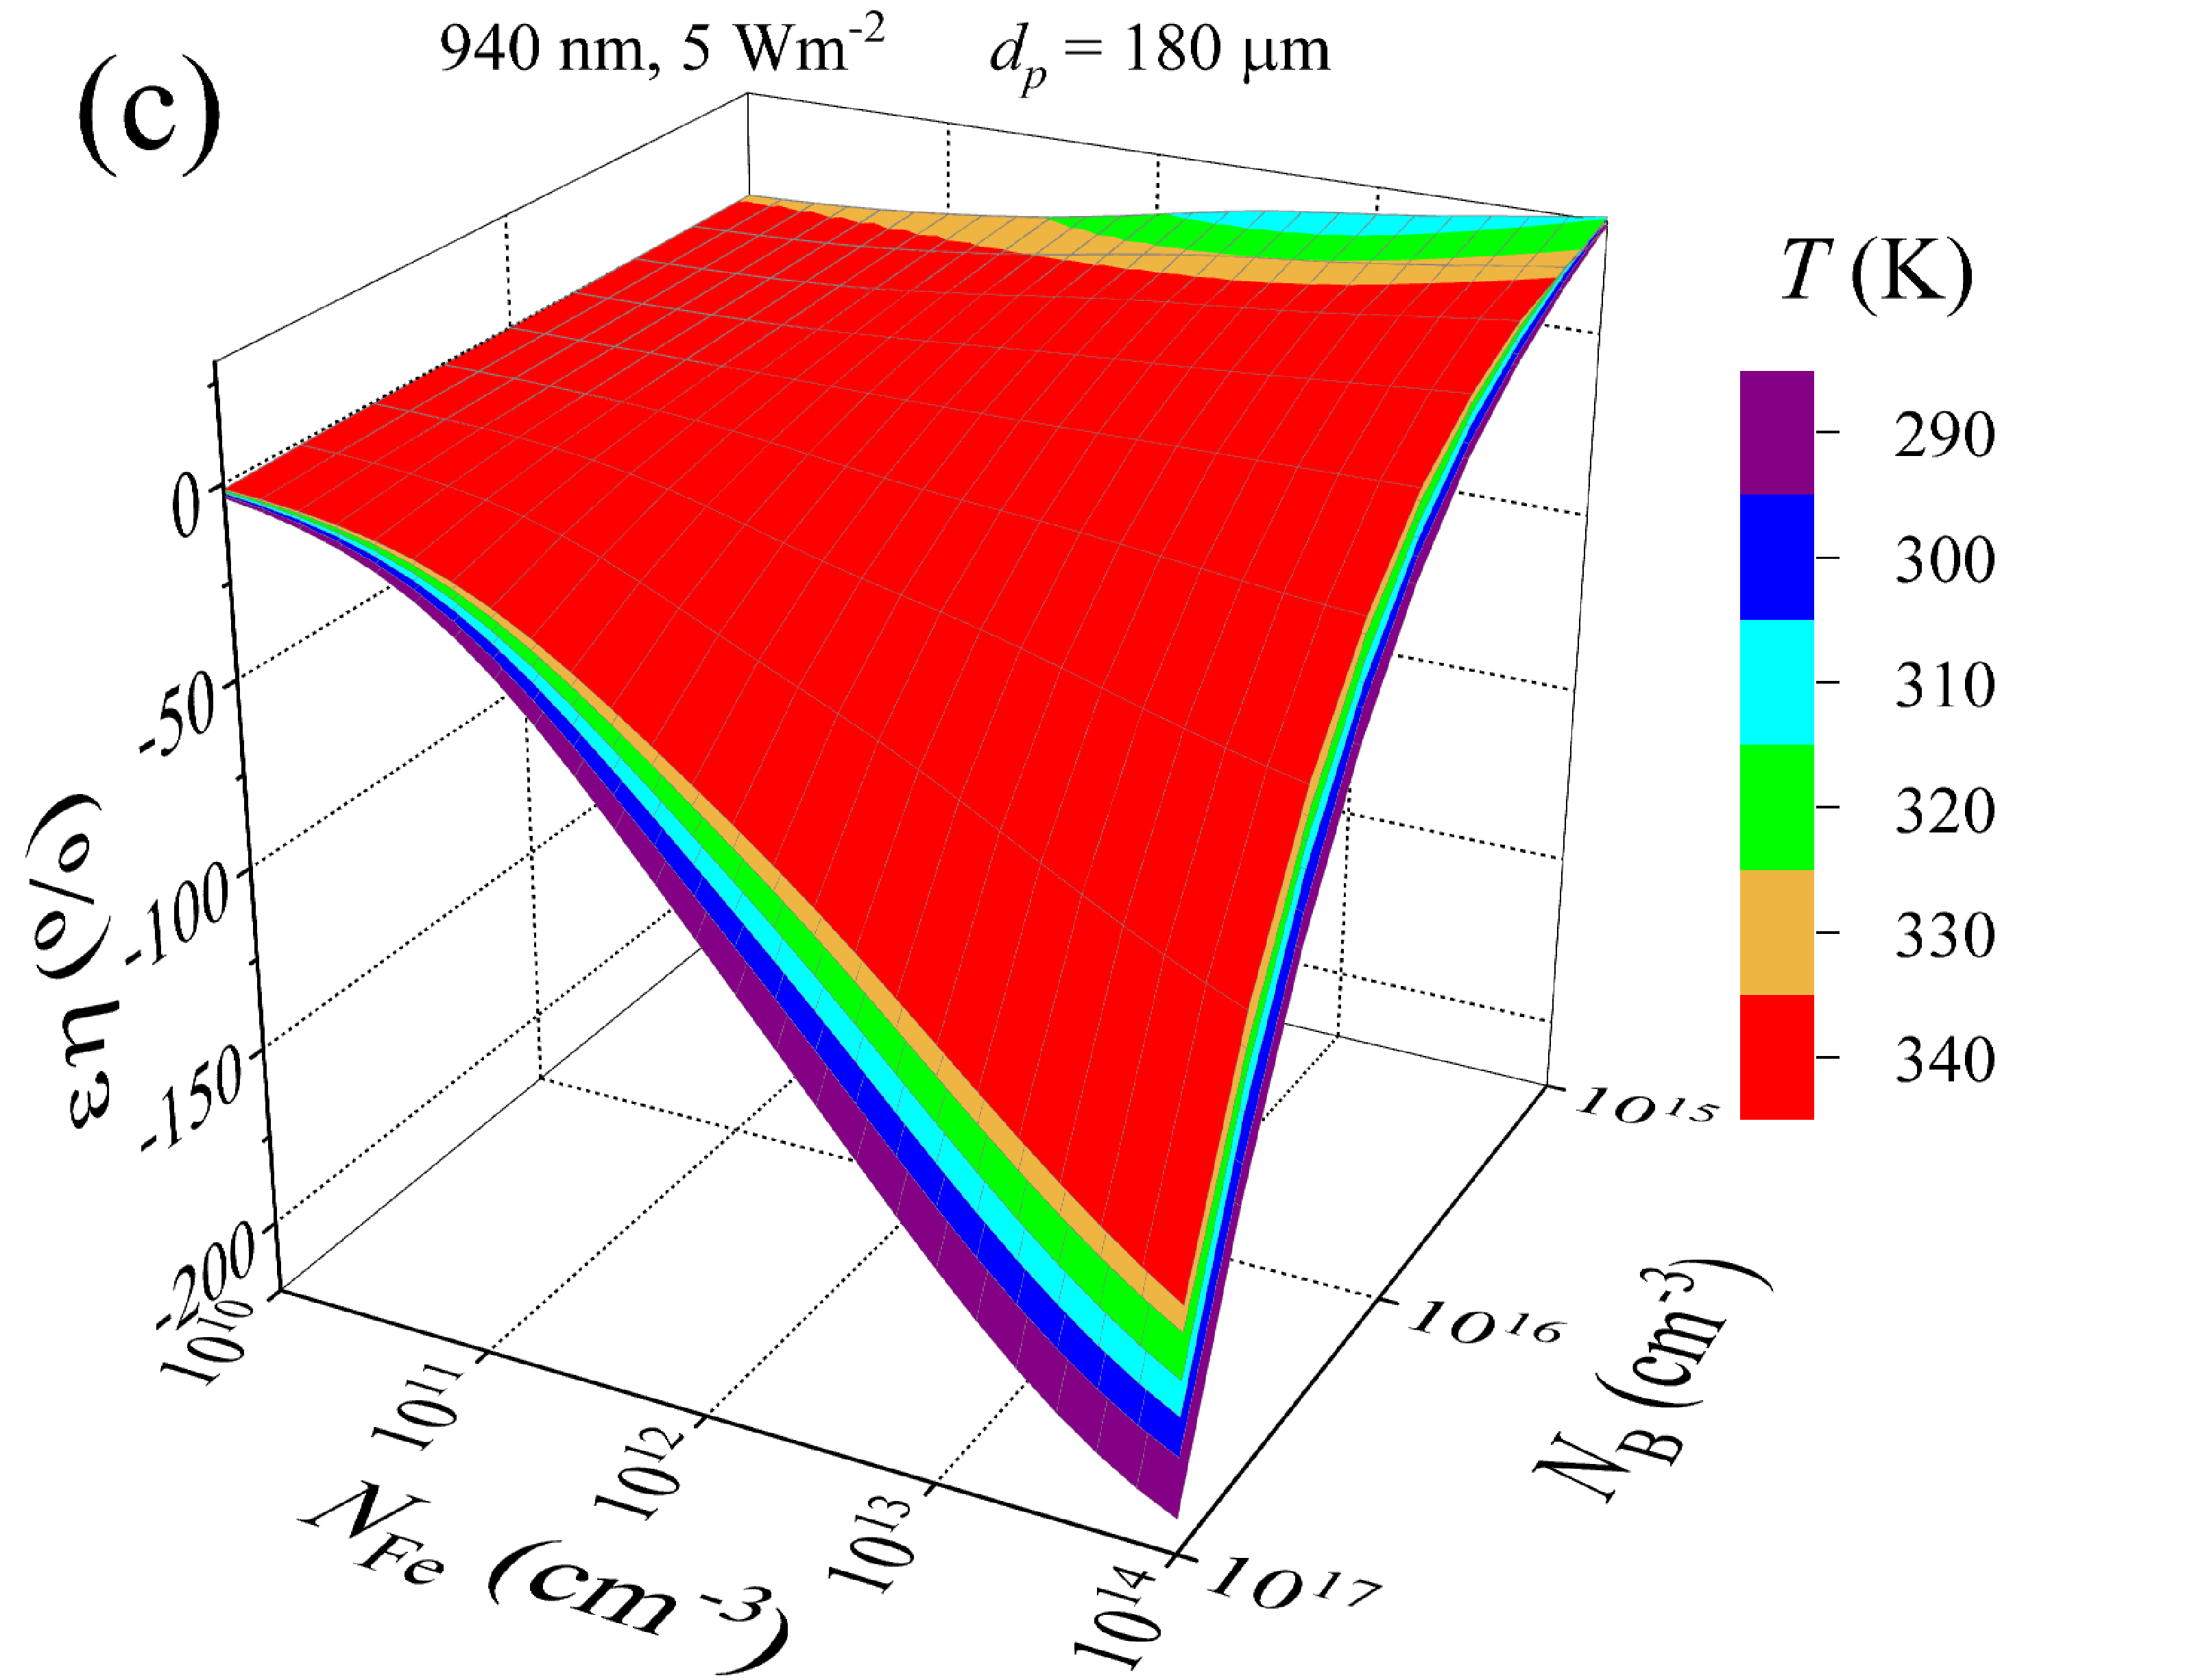
\includegraphics[width=0.49\linewidth]{Fig10c.png}
     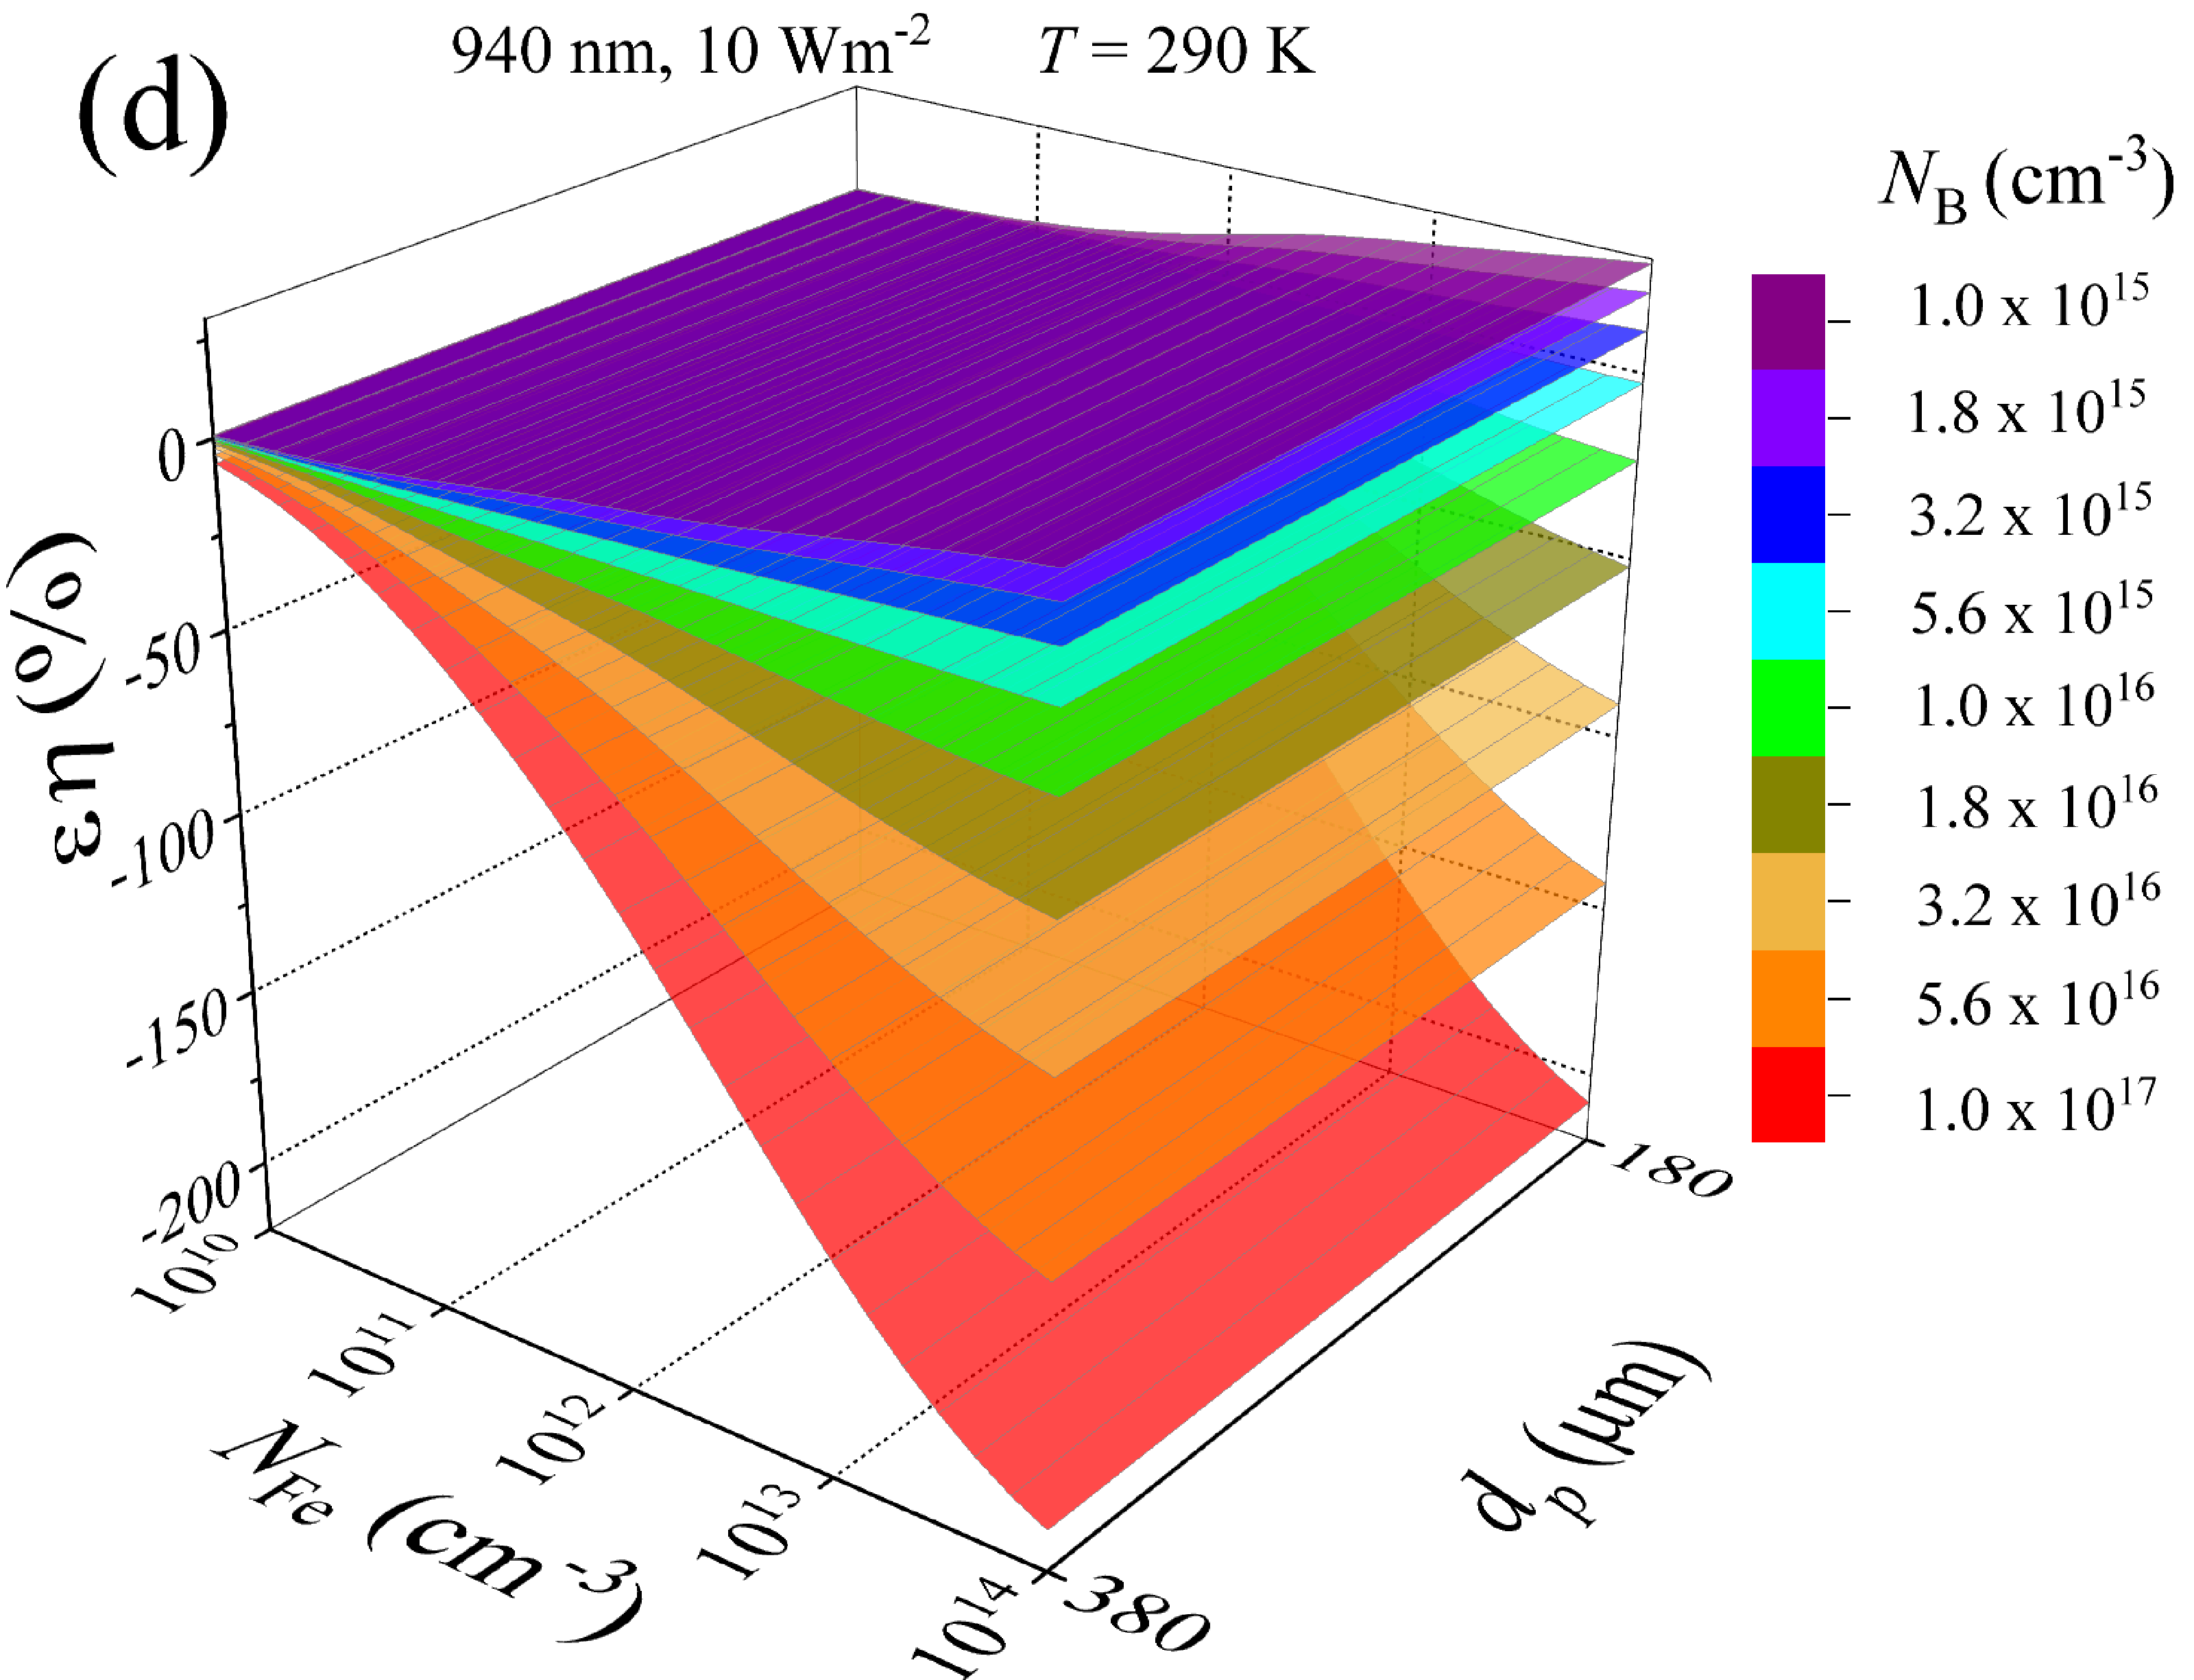
\includegraphics[width=0.49\linewidth]{Fig10d.png}
	  \caption{Relative changes in SSC efficiency caused by a complete
       dissociation of Fe$_i$B$_s$ pairs as a function of
       iron concentration and
       doping level (panels a and c) or base depth (b, d).
       Illumination: AM1.5 (a, b), 940~nm 5~Wm$^{-2}$ (c),  940~nm 10~Wm$^{-2}$ (d).
       $T$, K: 290 (d), 340 (b).
       $d_p$, $\mu$m: 180 (a, c).
       Different surfaces correspond to different temperatures (a, c) and doping levels (b, d).
}\label{fig10}
\end{figure}

The data indicate that the primary features of the $\varepsilon \eta$ dependencies
on solar cell parameters and temperature align with those observed for $\varepsilon I_\mathrm{SC}$.
However, a few differences are evident:
1)~the amplitude of  $\varepsilon \eta$ is enhanced,
reaching up to 50\% for AM1.5 and 200\% for 940~nm;
these results align with the expectations from Eq.~(\ref{eq12})
and make eta more convenient for iron concentration estimating;
2)~for AM1.5, in the region $N_\mathrm{B}<5\times10^{15}$~cm$^{-3}$,
a non-monotonic dependence of $\varepsilon \eta$$\left(N_\mathrm{Fe}\right)$ is observed,
rendering it impossible to use relative changes in efficiency as the sole parameter for iron concentration estimating under specified conditions;
3)~the existing dependence of $\varepsilon \eta$ on the intensity of the monochromatic illumination is weak,
which does not prevent the use of $\varepsilon \eta$ for determining $N_\mathrm{Fe}$, even with not very precise $W_\mathrm{ill}$ measurements;
4)~the temperature dependence of $\varepsilon \eta$ is weaker than that of $\varepsilon I_\mathrm{SC}$.


Fig.~\ref{fig11} shows the experimental and simulated values of changes in the efficiency of the solar cell
with a 380~$\mu$m base thickness and a doping concentration of $1.36\times10^{15}$~cm$^{-3}$.
When presenting the experimental data, the same correction factor, $C_\mathrm{cor} = 1.4$, was applied as in the case of the short-circuit current.
The data align closely, indicating that the inaccuracies typical for $V_\mathrm{OC}$ and $F\!F$  do not significantly contribute.

\begin{figure}
	\centering
     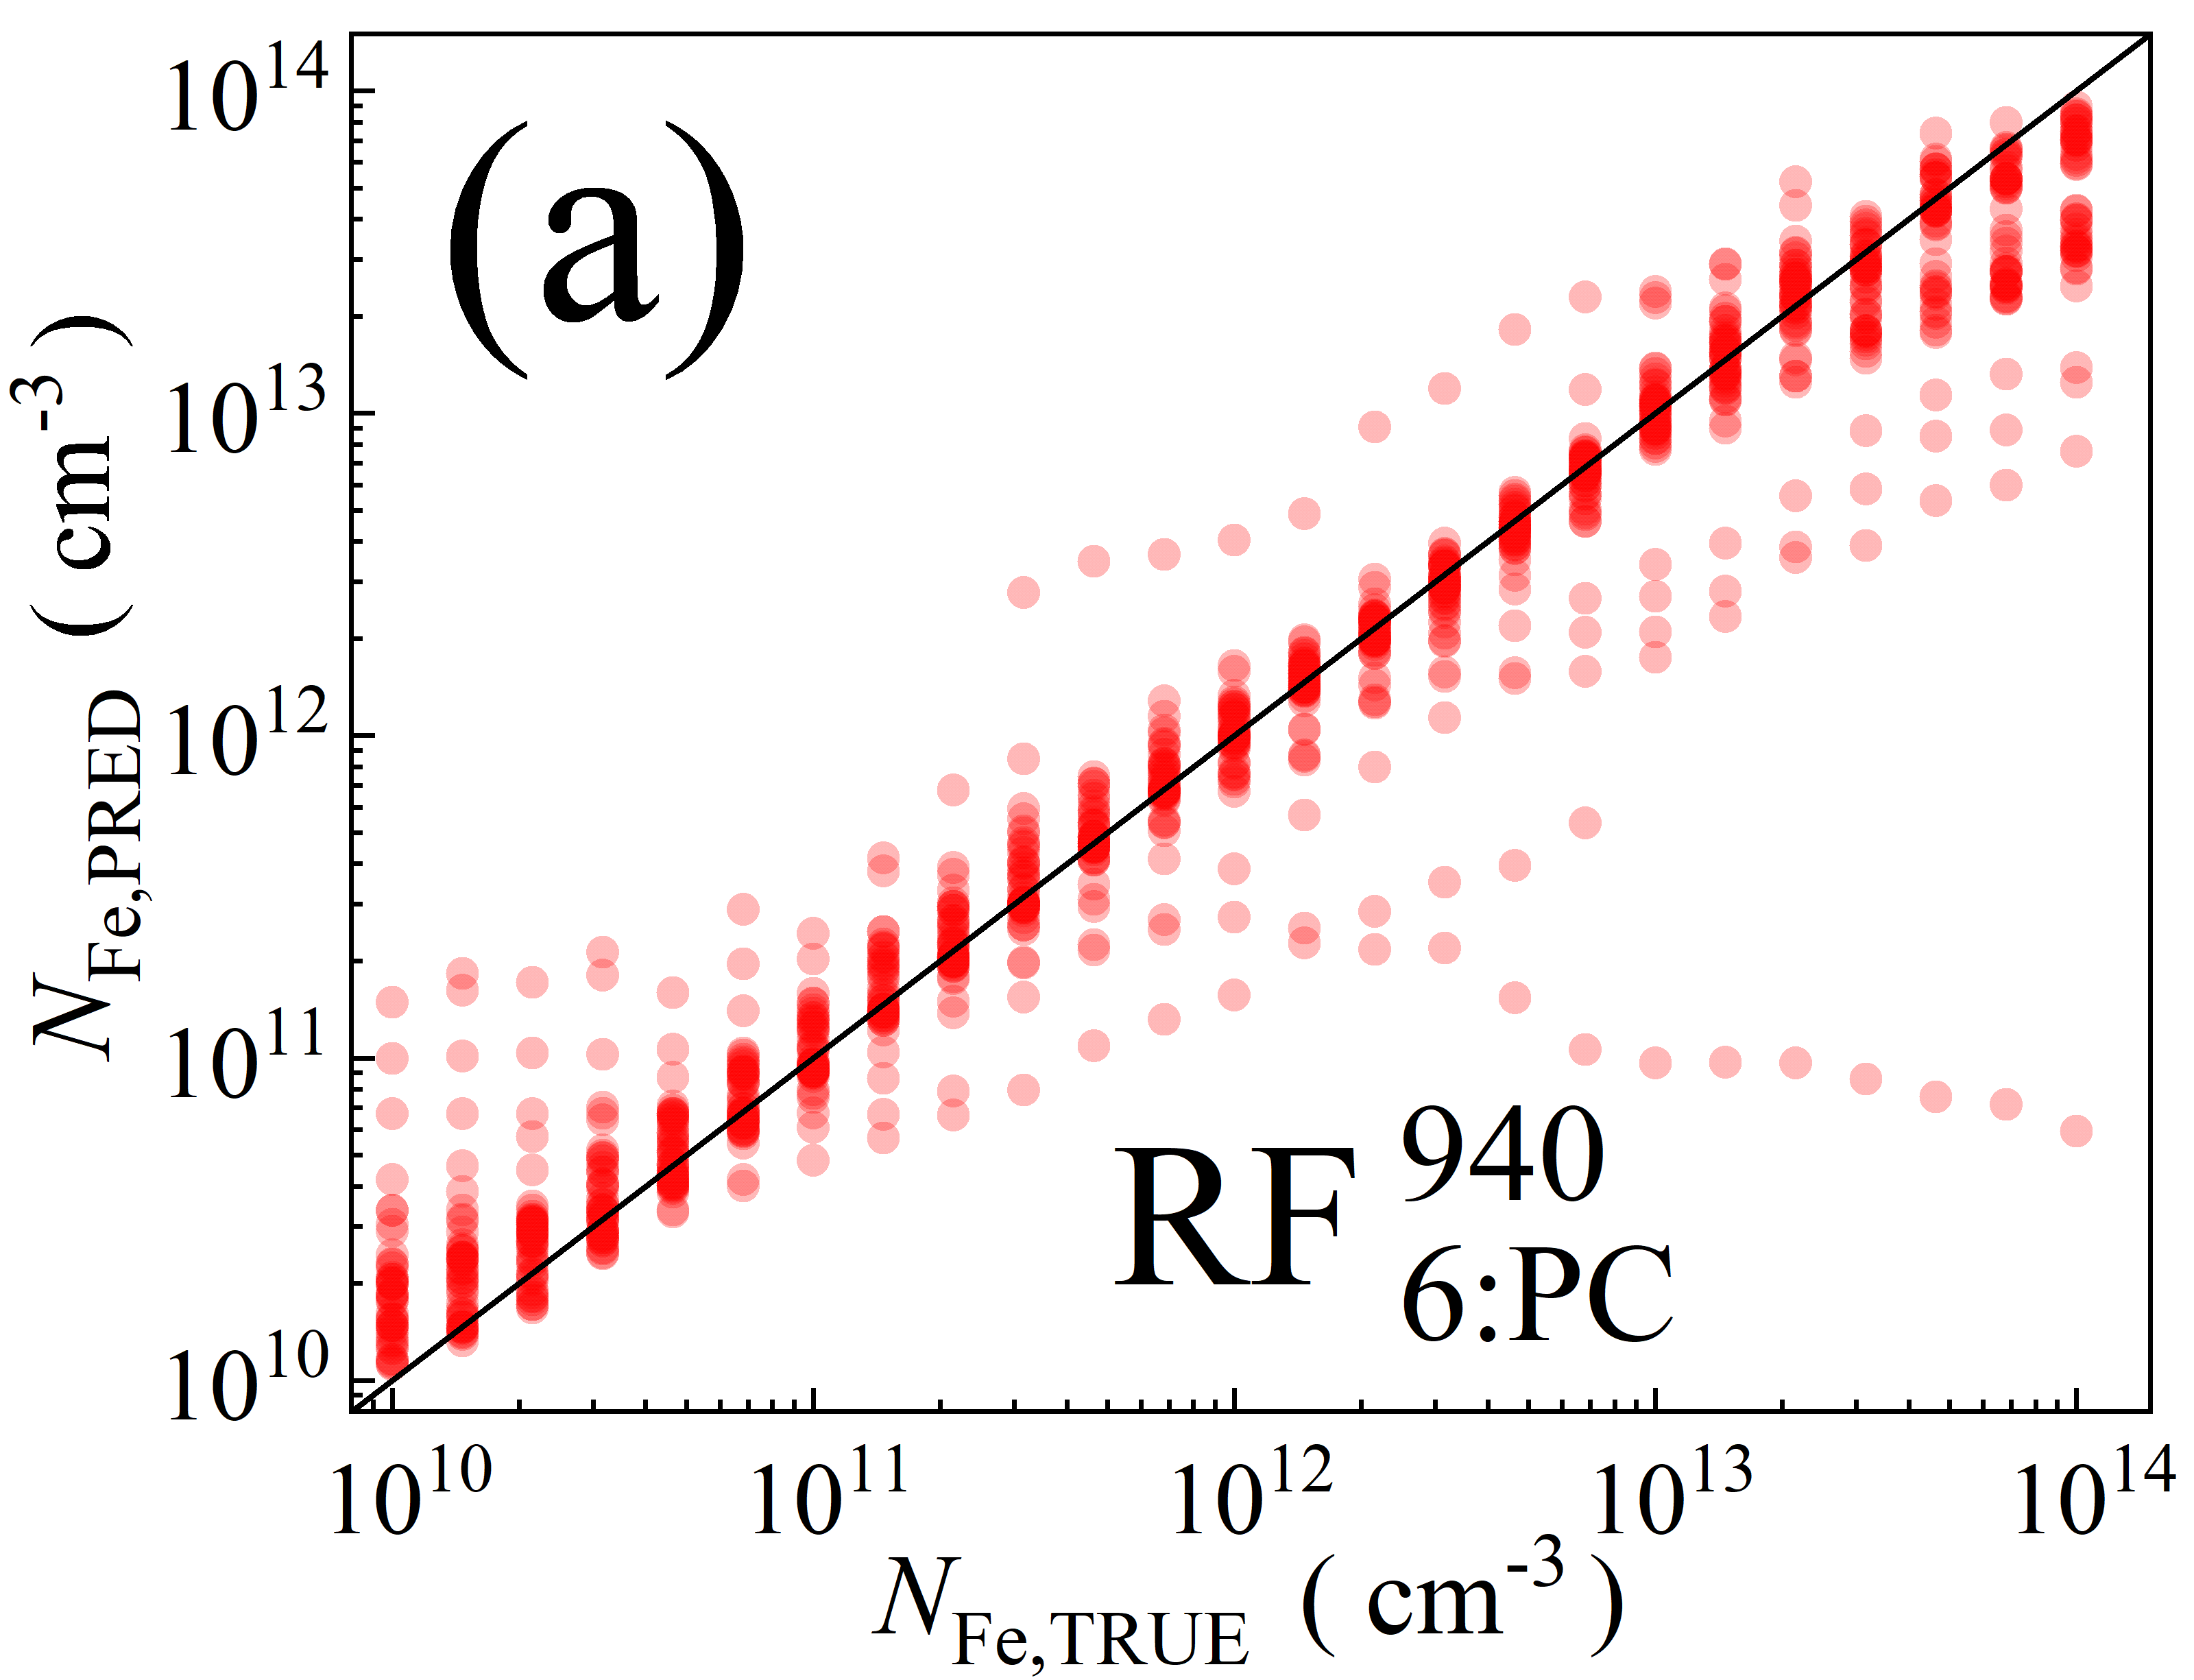
\includegraphics[width=0.4\linewidth]{Fig11a.png}
     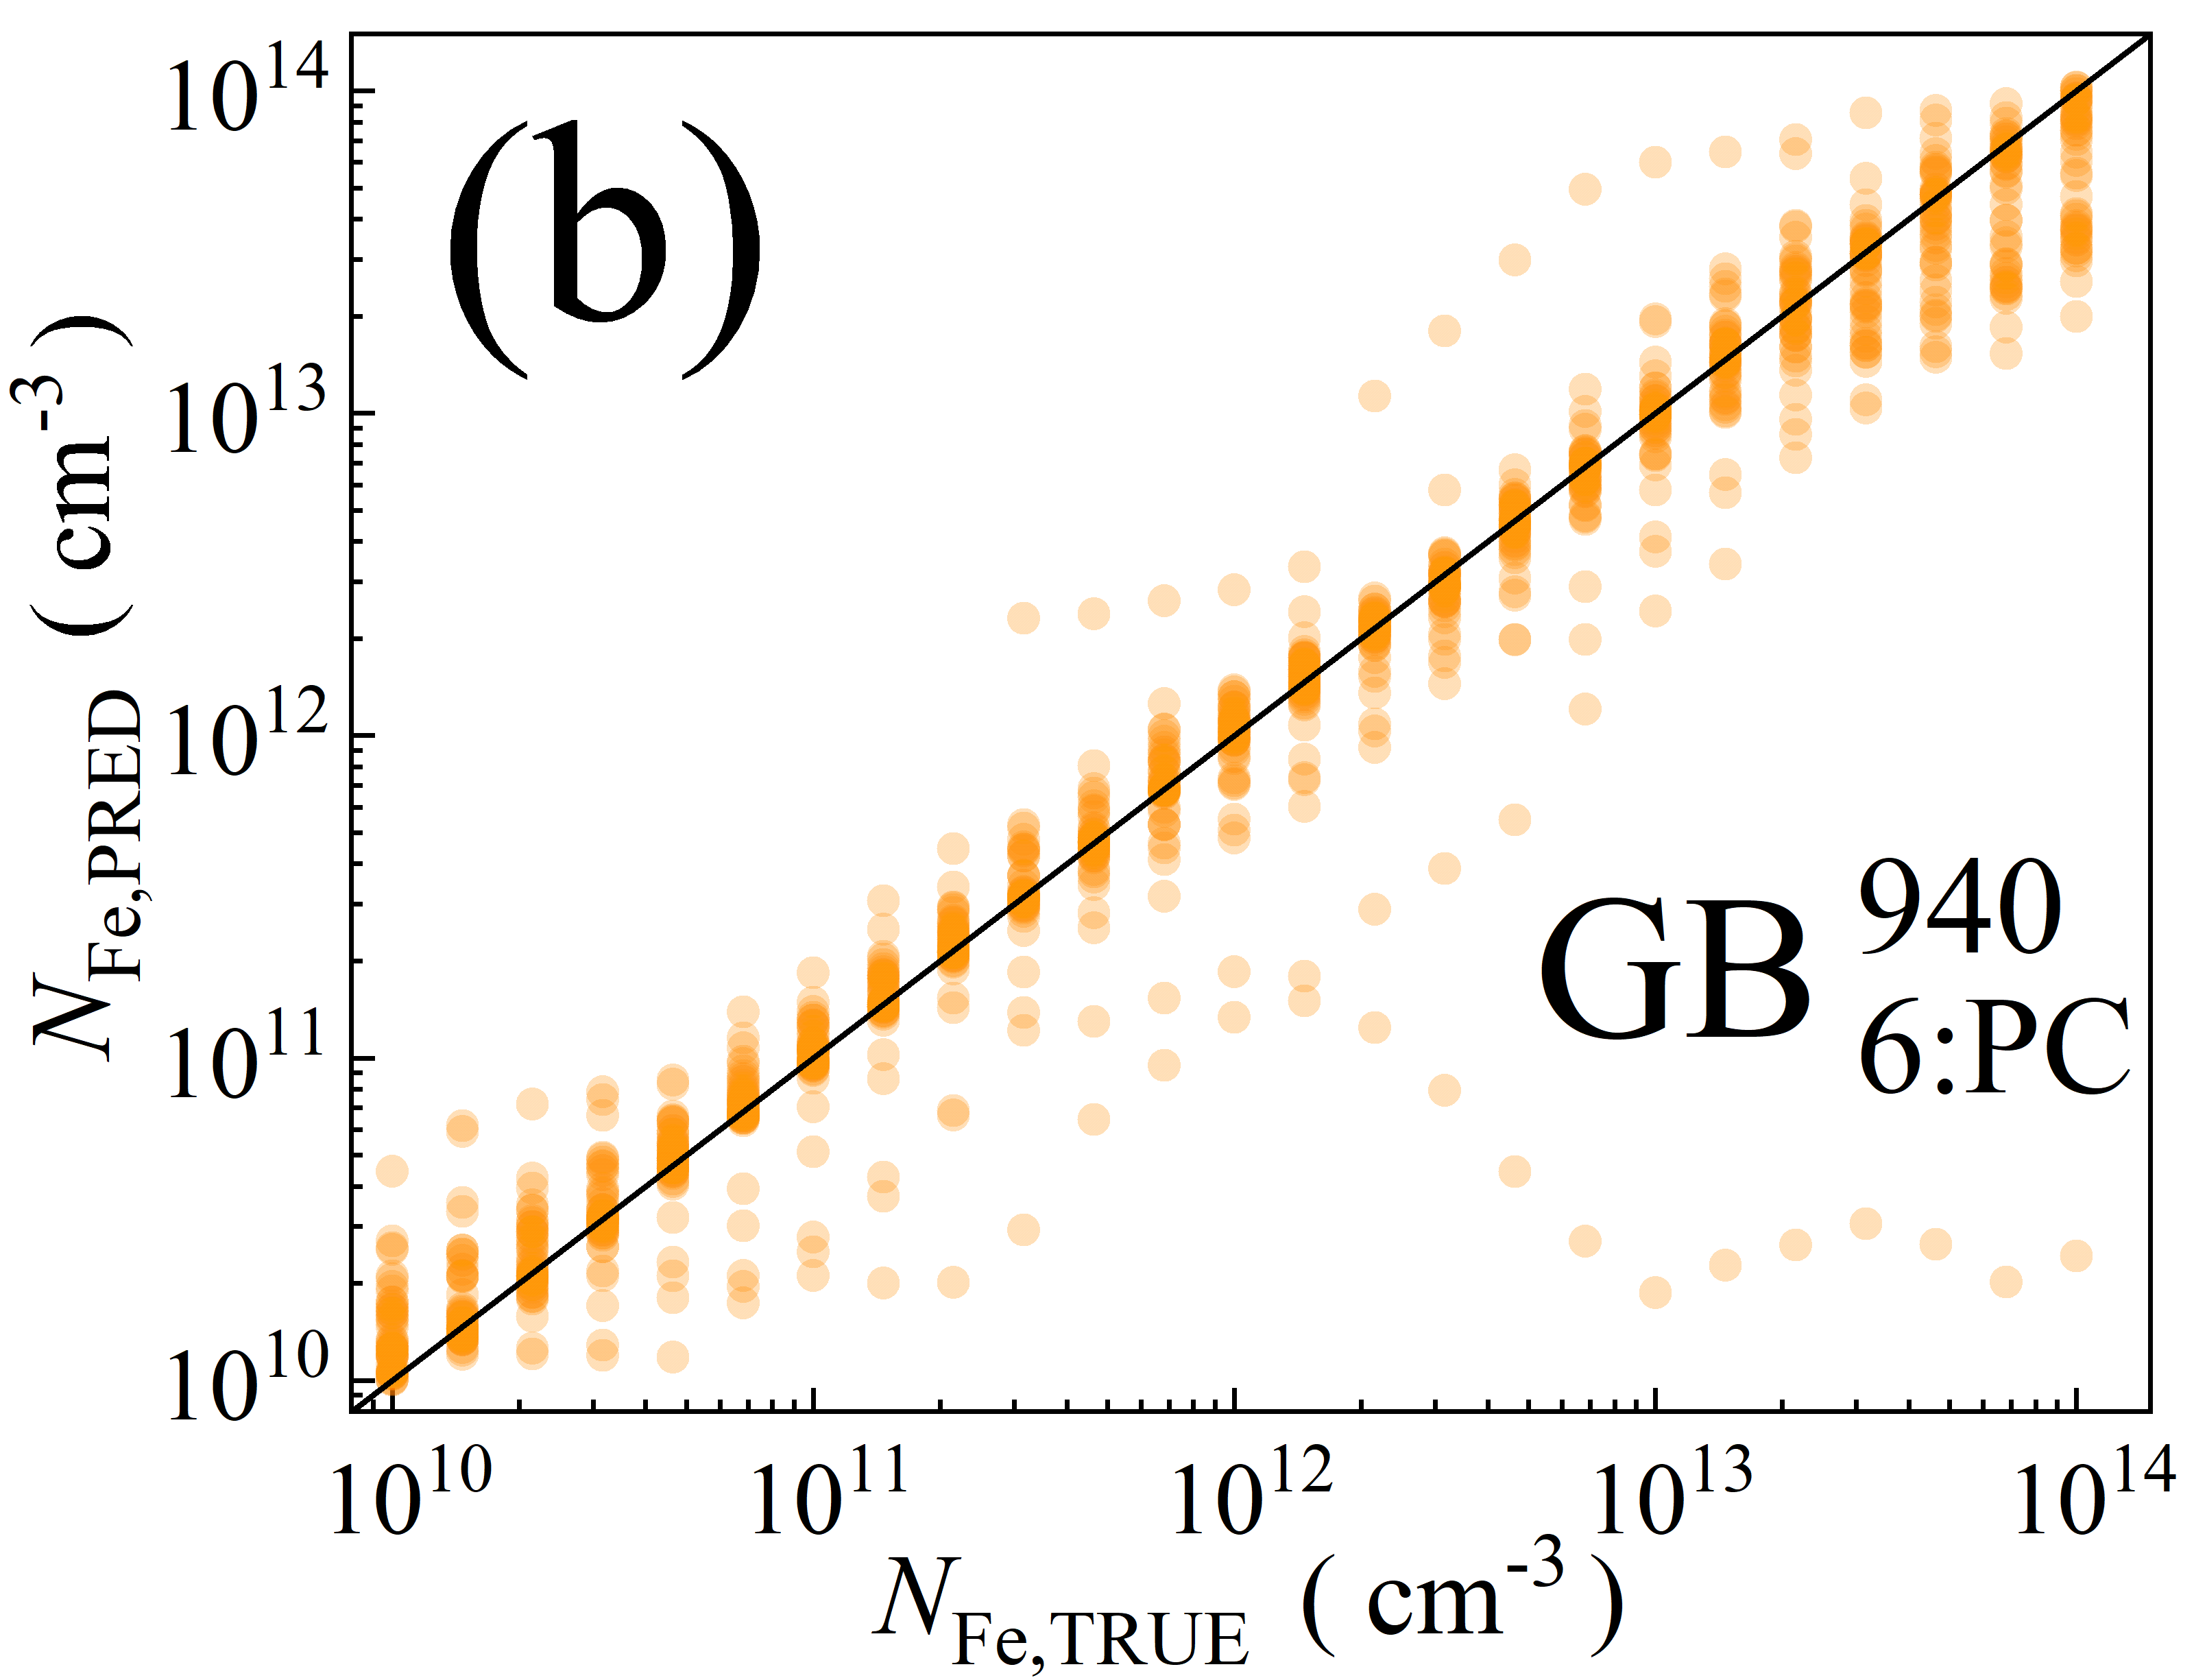
\includegraphics[width=0.4\linewidth]{Fig11b.png}
	  \caption{Relative changes in SSC efficiency caused by a complete
       dissociation of Fe$_i$B$_s$ pairs as a function of iron concentration (a) and
       temperature (b) for SSC with $d_p=380$~$\mu$m and $N_\mathrm{B}=1.36\times10^{15}$~cm$^{-3}$
       in the case of monochromatic (940~nm) illumination.
       The marks are the experimental results (divided by factor $C_{cor}=1.4$), the lines are the simulation results.
       $W_\mathrm{ill}$, Wm$^{-2}$: 5 (marks and solid lines), 10 (dotted lines).
       Different lines and marks correspond to different temperatures (a) or $N_\mathrm{Fe}$ values (b) --- see legends.
}\label{fig11}
\end{figure}

Obviously, the $\varepsilon \eta$ value can be used simultaneously with $\varepsilon I_\mathrm{SC}$ for a more accurate determination of iron concentration.
It is known that in machine learning, the input parameters typically consist of a set of variables (descriptors).
In our case, such a set could be ($T$, $d_p$, $N_\mathrm{B}$, $\varepsilon I_\mathrm{SC}$, $\varepsilon \eta$).
At the same time, if we compare Fig.~\ref{fig3} and Fig.~\ref{fig10},
we cannot expect that the values of $\varepsilon I_\mathrm{SC}$ and $\varepsilon \eta$ are independent.
To assess the redundancy of information, we can use principal component analysis (PCA),
widely used in solving various problems, including identifying defects in solar cells \cite{Fadhel2019}.
PCA uses a linear combination of the original variables to build the new variables (principal component, PC) while keeping maximum variance information.
In the case of the particular principal component having a low information variance ratio, it can be discarded with little to no loss of useful information.

PCs were built for different combinations of photovoltaic parameters and solar cell characteristics
for the full set of simulated data, and the results are listed in Table~\ref{tbl2}.
As evident, when only changes in short-circuit current are considered along with the solar cell's base parameters and temperature,
there is no excessive information present.
Adding $\varepsilon \eta$ to the set of descriptors practically does not change the number of independent variables.
With the additional use of $\varepsilon V_\mathrm{OC}$ values obtained under AM1.5 illumination, it is advisable to consider five independent variables.
For the same set of descriptors in a monochromatic illumination case, one can limit oneself to using only four independent components
(cumulative variance ratio for PC4 and PC5 does not exceed 1.3\%).
When considering changes in all photoelectric parameters due to complete dissociation of Fe$_i$B$_s$ pairs,
the actual number of independent variables is six for AM1.5 illumination and five for 940 nm lighting.


\begin{table}[<options>]
\caption{PSA results for sets of variables that serve to estimate the iron concentration in SSC.
The numbers represent the ratio of information variance associated with each principal component when using AM1.5 illumination / 940 nm illumination.
}
\label{tbl2}
\begin{tabular*}{\tblwidth}{@{}LCCCCCCC@{}}
\toprule
set of descriptors&\multicolumn{7}{C}{Explained Variance Ratio (\%)}\\
&PC0&PC1&PC2&PC3&PC4&PC5&PC6\\% Table header row
\midrule
%($T$, $d_p$, $N_\mathrm{B}$, $\varepsilon I_\mathrm{SC}$)&43.23&25.00&25.00&6.70&---&---&---\\
%($T$, $d_p$, $N_\mathrm{B}$, $\varepsilon I_\mathrm{SC}$, $\varepsilon \eta$) & 52.39 &20.00&20.00&7.48&0.13& ---&---\\
%($T$, $d_p$, $N_\mathrm{B}$, $\varepsilon I_\mathrm{SC}$, $\varepsilon \eta$, $\varepsilon V_\mathrm{OC}$) & 44.40 &18.78&16.67&16.46&3.61& 0.08&---\\
%($T$, $d_p$, $N_\mathrm{B}$, $\varepsilon I_\mathrm{SC}$, $\varepsilon \eta$, $\varepsilon V_\mathrm{OC}$, $\varepsilon FF$) & 43.29 &22.59&14.29&14.19&4.29& 1.35&0.002\\
($T$, $d_p$, $N_\mathrm{B}$, $\varepsilon I_\mathrm{SC}$)&43.23/42.80&25.00/25.00&25.00/25.00&6.70/7.20&---&---&---\\
($T$, $d_p$, $N_\mathrm{B}$, $\varepsilon I_\mathrm{SC}$, $\varepsilon \eta$) & 52.39/52.46 &20.00/20.00&20.00/20.00&7.48/7.51&0.13/0.03& ---&---\\
($T$, $d_p$, $N_\mathrm{B}$, $\varepsilon I_\mathrm{SC}$, $\varepsilon \eta$, $\varepsilon V_\mathrm{OC}$) & 44.40/59.02 &18.78/16.73&16.67/16.67&16.46/6.28&3.61/1.29& 0.08/0.01&---\\
($T$, $d_p$, $N_\mathrm{B}$, $\varepsilon I_\mathrm{SC}$, $\varepsilon \eta$, $\varepsilon V_\mathrm{OC}$, $\varepsilon F\!F$) & 43.29/63.24 &22.59/14.41&14.29/14.29&14.19/5.65&4.29/1.95& 1.35/0.46&0.002/0.01\\
\bottomrule
\end{tabular*}
\end{table}



\section{Conclusion}

We have provided the results of modeling the impact of variations in the
state of iron impurities on the photovoltaic parameters of silicon solar cells
with different base properties under various external conditions
(temperature, intensity, and spectral composition of illumination).
The simulation results have been compared with experimental data.

The feasibility of using relative changes in short-circuit current, open-circuit voltage,
fill factor, and efficiency resulting from the dissociation of FeB pairs
to estimate the concentration of iron impurities in a solar cell has been analyzed.
It is shown that changes in short-circuit current are the most suitable parameter.
It is more expedient to determine the photovoltaic parameters under monochromatic illumination
with a wavelength matching the predominant absorption in the solar cell base rather than using AM1.5 illumination.
Next in suitability are changes in efficiency and open-circuit voltage,
although their use becomes restricted at low doping levels of the base ($<10^{16}$~cm$^{-3}$).
In our opinion, using the fill factor to estimate iron concentration is not practical.

It has been shown that the potential accuracy of estimating iron concentration depends
on the doping level of the base:
at a boron concentration around $10^{16}$~cm$^{-3}$, it is minimal,
while decreasing or increasing this value enhances the response of $I_\mathrm{SC}$ to the presence of iron.
Furthermore, the accuracy of $N_\mathrm{Fe}$ determination is significantly influenced by the availability
of precise information on the doping level of the base,
as well as the accuracy of estimating the intensity of monochromatic illumination,
especially when using $\varepsilon \eta$ and $\varepsilon V_\mathrm{OC}$.

At the same time, $\varepsilon \eta$ and $\varepsilon V_\mathrm{OC}$ can serve as additional parameters
for refining the determination of iron concentration.
In our opinion, for estimating iron concentration through changes
in photovoltaic parameters due to variability in iron-related defects, it is advisable to use a set of
($T$, $d_p$, $N_\mathrm{B}$, $\varepsilon I_\mathrm{SC}$, $\varepsilon \eta$) or ($T$, $d_p$, $N_\mathrm{B}$, $\varepsilon I_\mathrm{SC}$, $\varepsilon \eta$,$\varepsilon V_\mathrm{OC}$).
In these cases, to expedite calculations, it is advisable to use principal component analysis to reduce
the number of variables while retaining the maximum variance information.



\section*{Acknowledgments}
O.O. would like to acknowledge the financial support by
National Research Foundation of Ukraine (Project No. 2023.03/0252
‘‘Development of principles for the creation and machine-oriented
characterization of porous silicon nanostructures with optimal
heat transport properties’’)

\section*{Supplementary data}\label{SuplData}
Supplementary data to this article can be found online at
%\url{http://surl.li/szpkwz}
\url{https://1ll.ink/01mfC}

\section*{Data availability}
Data will be made available on request.


% To print the credit authorship contribution details
%\printcredits

%% Loading bibliography style file
\bibliographystyle{model1-num-names}

%\bibliographystyle{cas-model2-names}

% Loading bibliography database
\bibliography{olikh}



\end{document}

%В реченні "" заміни, будь-ласка, "" для підвищення clarity
%В реченні "" заміни, будь-ласка, "" для підвищення conciseness
%В реченні "" заміни, будь-ласка, "" для підвищення  sensitivity

